\RequirePackage[l2tabu,orthodox]{nag}

\documentclass[bachelors,a4paper]{chalmers-thesis}

\usepackage[swedish, english]{babel}

\usepackage[utf8]{inputenc}
\usepackage{comment}
\usepackage{color}
\usepackage{todonotes}
\usepackage{hyperref}


% To be able to include pdfs in the document
\usepackage{pdfpages}

% To use appendices
\usepackage[toc,page]{appendix}

% Fancy maths!
\usepackage{amsmath}
\usepackage{amssymb}

% Fancy references
\usepackage[style=authoryear,date=iso8601]{biblatex}
\addbibresource{jelzin.bib}

% Fancy graphics
\usepackage{graphicx}

% For the finest tables
\usepackage{booktabs}
\usepackage{longtable}

% For mutliple column pages
\usepackage{multicol}

% For the finest of subfigures in figures or tables
\usepackage{subcaption}

% To be able to position figure envs exactly where you want them use H.
\usepackage{float}

% Nice environments for pseudocode
\usepackage[chapter]{algorithm}
\usepackage{algpseudocode}

\title{Reinforcement learning}
\subtitle{A comparison of agents in discrete environments with large discrete state spaces using reinforcement learning.}
\author{%
Johan Andersson \and
Emil Kristiansson \and
Joakim Persson \and
Adam Sandberg Eriksson \and
Daniel Toom \and
Joppe Widstam
}
\thesisin{Computer Science}
\department{Department of Computer Science and Engineering}
\reportno{2014:05}
\copyrightyear{2014}
\keywords{Reinforcement learning, Artificial intelligence}

% Abstracts
\firstabstract{% 1 Motivation

For some real-world behavior optimization problems, it is infeasible to search for a solution by making a model of the problem and performing calculations on it. 
In cases like these, good solutions can sometimes be found by trial and error. 
Reinforcement learning is a way of finding optimal behavior by systematic trial and error.
% 2 Problem statement
This thesis aims to compare different reinforcement learning techniques and evaluate them. 
Model-based interval estimation (MBIE) and Explicit explore or exploit using dynamic bayesian networks - (DBN-\etre)
 are two algorithms that are evaluated. 
% 3 Approach
To evaluate the techniques, learning agents were constructed using the algorithms and 
then simulated in the environment invasive species from the reinforcement learning competition.
% 4 Results
The results of the study show that an optimized version of DBN-\etre\ is better than MBIE at finding an optimal or near optimal behavior policy in the 
environment invasive species for a selection of environment parameters.

% 5 Conclusions
Using a factored model like a DBN shows certain advantages operating in 
the factored environment invasive species. For example it achieves a near optimal
policy within fewer episodes than MBIE.


% Följande saker ska vara med i en abstract Motivation, Problem Statement, Approach, REsults

% Motivation
% Why do we care about the problem and the results? 
% If the problem isn't obviously "interesting" it might be better to
% put motivation first; but if your work is incremental progress on
% a problem that is widely recognized as important, then it is 
% probably better to put the problem statement first to indicate which
%  piece of the larger problem you are breaking off to work on.
% This section should include the importance of your work, the difficulty
% of the area, and the impact it might have if successful.

% Problem statement
% What problem are you trying to solve? What is the scope of your work 
%(a generalized approach, or for a specific situation)? Be careful not to 
% use too much jargon. In some cases it is appropriate to put the problem 
% statement before the motivation, but usually this only works if most 
% readers already understand why the problem is important.

% Approach
% How did you go about solving or making progress on the problem? Did you 
% use simulation, analytic models, prototype construction, or analysis of
% field data for an actual product? What was the extent of your work
% (did you look at one application program or a hundred programs in
% twenty different programming languages?) What important variables did
% you control, ignore, or measure?

% Results
% What's the answer? Specifically, most good computer architecture papers 
% conclude that something is so many percent faster, cheaper, smaller, 
% or otherwise better than something else. Put the result there, in
% numbers. Avoid vague, hand-waving results such as "very", "small",
% or "significant." If you must be vague, you are only given license
% to do so when you can talk about orders-of-magnitude improvement. 
% There is a tension here in that you should not provide numbers that
% can be easily misinterpreted, but on the other hand you don't have
% room for all the caveats.

% Conclusions
% What are the implications of your answer? Is it going to change the 
% world (unlikely), be a significant "win", be a nice hack, or simply 
% serve as a road sign indicating that this path is a waste of time 
% (all of the previous results are useful). Are your results general, 
% potentially generalizable, or specific to a particular case?
}
\secondabstract{swedish}{% 1 Motivation
För vissa verklighetsbaserade optimeringsproblem där det gäller att finna ett bästa beteende är det orimligt söka efter det optimala beteendet genom att skapa en modell av problemet och sedan utföra beräkningar på den. I vissa sådana fall kan man hitta bra lösningar genom trial and error. Reinforcement learning är ett sätt att hitta optimalt beteende genom att systematisk pröva sig fram.
% 2 Problem statement
Detta kandidatarbete har som mål att jämföra olika inlärningstekniker och utvärdera dessa.
Model-based interval estimation (MBIE) och Explicit Explore or Exploit med dynamiska bayesnät (DBN-\etre) är 
två självlärande algoritmer som här utvärderas.

% 3 Approach
För att utvärdera de olika teknikerna implementerades agenter som använde algoritmerna, och dessa testkördes sedan 
i miljön invasive species från tävlingen Reinforcement learning competition.

% 4 Results
DBN-\etre\ är bättre än MBIE på att hitta en optimal eller nära optimal policy i miljön invasive species med valda parametrar.
% 5 Conclusions
Att använda en faktoriserad model, så som DBN-\etre\, visar på tydliga fördelar i faktoriserade miljöer, som i till exempel invasive species. 
Ett exempel på detta är att den når en nästan optimal policy på färre episoder än MBIE.

% Följande saker ska vara med i en abstract Motivation, Problem Statement, Approach, REsults

% Motivation
% Why do we care about the problem and the results? 
% If the problem isn't obviously "interesting" it might be better to
% put motivation first; but if your work is incremental progress on
% a problem that is widely recognized as important, then it is 
% probably better to put the problem statement first to indicate which
%  piece of the larger problem you are breaking off to work on.
% This section should include the importance of your work, the difficulty
% of the area, and the impact it might have if successful.

% Problem statement
% What problem are you trying to solve? What is the scope of your work 
%(a generalized approach, or for a specific situation)? Be careful not to 
% use too much jargon. In some cases it is appropriate to put the problem 
% statement before the motivation, but usually this only works if most 
% readers already understand why the problem is important.

% Approach
% How did you go about solving or making progress on the problem? Did you 
% use simulation, analytic models, prototype construction, or analysis of
% field data for an actual product? What was the extent of your work
% (did you look at one application program or a hundred programs in
% twenty different programming languages?) What important variables did
% you control, ignore, or measure?

% Results
% What's the answer? Specifically, most good computer architecture papers 
% conclude that something is so many percent faster, cheaper, smaller, 
% or otherwise better than something else. Put the result there, in
% numbers. Avoid vague, hand-waving results such as "very", "small",
% or "significant." If you must be vague, you are only given license
% to do so when you can talk about orders-of-magnitude improvement. 
% There is a tension here in that you should not provide numbers that
% can be easily misinterpreted, but on the other hand you don't have
% room for all the caveats.

% Conclusions
% What are the implications of your answer? Is it going to change the 
% world (unlikely), be a significant "win", be a nice hack, or simply 
% serve as a road sign indicating that this path is a waste of time 
% (all of the previous results are useful). Are your results general, 
% potentially generalizable, or specific to a particular case?
}

% Useful commands
\newcommand{\note}[1]{\textcolor{red}{#1}}
\newcommand{\etre}{\ensuremath{E^3}}

\begin{document}

\makecoverpage
\maketitlepage
\makeprintinfopage

\newpage

\pagenumbering{roman}
\pagestyle{plain}

\makeabstractpage
\makesecondabstractpage

\todo[inline]{Make sure the title and text of each section match}
\todo[inline]{Look over the size of all the paragraphs in the world)}
\todo[inline]{Be consistent with reinforcement learning (not Reinforcement Learning, RL)}
\todo[inline]{Be consistent in introductions using references to subsections}
\todo[inline]{Check see section vs section, and same w figure}
\todo[inline]{Tamarisk -> tamarix}

\newpage

\listoftodos

\tableofcontents

\newpage

\pagenumbering{arabic}

\RequirePackage[l2tabu,orthodox]{nag}

\documentclass[bachelors,a4paper]{chalmers-thesis}

\usepackage[swedish, english]{babel}

\usepackage[utf8]{inputenc}
\usepackage{comment}
\usepackage{color}
\usepackage{todonotes}
\usepackage{hyperref}


% To be able to include pdfs in the document
\usepackage{pdfpages}

% To use appendices
\usepackage[toc,page]{appendix}

% Fancy maths!
\usepackage{amsmath}
\usepackage{amssymb}

% Fancy references
\usepackage[style=authoryear,date=iso8601]{biblatex}
\addbibresource{jelzin.bib}

% Fancy graphics
\usepackage{graphicx}

% For the finest tables
\usepackage{booktabs}
\usepackage{longtable}

% For mutliple column pages
\usepackage{multicol}

% For the finest of subfigures in figures or tables
\usepackage{subcaption}

% To be able to position figure envs exactly where you want them use H.
\usepackage{float}

% Nice environments for pseudocode
\usepackage[chapter]{algorithm}
\usepackage{algpseudocode}

\title{Reinforcement learning}
\subtitle{A comparison of learning agents in environments with large discrete state spaces}
\author{%
Johan Andersson\and
Emil Kristiansson\and
Joakim Persson\and
Adam Sandberg Eriksson\and
Daniel Toom\and
Joppe Widstam}
\thesisin{Computer Science}
\department{Department of Computer Science and Engineering}
\reportno{2014:05}
\copyrightyear{2014}
\keywords{Reinforcement learning, Artificial intelligence, MBIE, DBN-\etre, Invasive Species, Learning algorithms}

% Abstracts
\firstabstract{% 1 Motivation

For some real-world behavior optimization problems, it is infeasible to search for a solution by making a model of the problem and performing calculations on it. 
In cases like these, good solutions can sometimes be found by trial and error. 
Reinforcement learning is a way of finding optimal behavior by systematic trial and error.
% 2 Problem statement
This thesis aims to compare different reinforcement learning techniques and evaluate them. 
Model-based interval estimation (MBIE) and Explicit explore or exploit using dynamic bayesian networks - (DBN-\etre)
 are two algorithms that are evaluated. 
% 3 Approach
To evaluate the techniques, learning agents were constructed using the algorithms and 
then simulated in the environment invasive species from the reinforcement learning competition.
% 4 Results
The results of the study show that an optimized version of DBN-\etre\ is better than MBIE at finding an optimal or near optimal behavior policy in the 
environment invasive species for a selection of environment parameters.

% 5 Conclusions
Using a factored model like a DBN shows certain advantages operating in 
the factored environment invasive species. For example it achieves a near optimal
policy within fewer episodes than MBIE.


% Följande saker ska vara med i en abstract Motivation, Problem Statement, Approach, REsults

% Motivation
% Why do we care about the problem and the results? 
% If the problem isn't obviously "interesting" it might be better to
% put motivation first; but if your work is incremental progress on
% a problem that is widely recognized as important, then it is 
% probably better to put the problem statement first to indicate which
%  piece of the larger problem you are breaking off to work on.
% This section should include the importance of your work, the difficulty
% of the area, and the impact it might have if successful.

% Problem statement
% What problem are you trying to solve? What is the scope of your work 
%(a generalized approach, or for a specific situation)? Be careful not to 
% use too much jargon. In some cases it is appropriate to put the problem 
% statement before the motivation, but usually this only works if most 
% readers already understand why the problem is important.

% Approach
% How did you go about solving or making progress on the problem? Did you 
% use simulation, analytic models, prototype construction, or analysis of
% field data for an actual product? What was the extent of your work
% (did you look at one application program or a hundred programs in
% twenty different programming languages?) What important variables did
% you control, ignore, or measure?

% Results
% What's the answer? Specifically, most good computer architecture papers 
% conclude that something is so many percent faster, cheaper, smaller, 
% or otherwise better than something else. Put the result there, in
% numbers. Avoid vague, hand-waving results such as "very", "small",
% or "significant." If you must be vague, you are only given license
% to do so when you can talk about orders-of-magnitude improvement. 
% There is a tension here in that you should not provide numbers that
% can be easily misinterpreted, but on the other hand you don't have
% room for all the caveats.

% Conclusions
% What are the implications of your answer? Is it going to change the 
% world (unlikely), be a significant "win", be a nice hack, or simply 
% serve as a road sign indicating that this path is a waste of time 
% (all of the previous results are useful). Are your results general, 
% potentially generalizable, or specific to a particular case?
}
\secondabstract{swedish}{% 1 Motivation
För vissa verklighetsbaserade optimeringsproblem där det gäller att finna ett bästa beteende är det orimligt söka efter det optimala beteendet genom att skapa en modell av problemet och sedan utföra beräkningar på den. I vissa sådana fall kan man hitta bra lösningar genom trial and error. Reinforcement learning är ett sätt att hitta optimalt beteende genom att systematisk pröva sig fram.
% 2 Problem statement
Detta kandidatarbete har som mål att jämföra olika inlärningstekniker och utvärdera dessa.
Model-based interval estimation (MBIE) och Explicit Explore or Exploit med dynamiska bayesnät (DBN-\etre) är 
två självlärande algoritmer som här utvärderas.

% 3 Approach
För att utvärdera de olika teknikerna implementerades agenter som använde algoritmerna, och dessa testkördes sedan 
i miljön invasive species från tävlingen Reinforcement learning competition.

% 4 Results
DBN-\etre\ är bättre än MBIE på att hitta en optimal eller nära optimal policy i miljön invasive species med valda parametrar.
% 5 Conclusions
Att använda en faktoriserad model, så som DBN-\etre\, visar på tydliga fördelar i faktoriserade miljöer, som i till exempel invasive species. 
Ett exempel på detta är att den når en nästan optimal policy på färre episoder än MBIE.

% Följande saker ska vara med i en abstract Motivation, Problem Statement, Approach, REsults

% Motivation
% Why do we care about the problem and the results? 
% If the problem isn't obviously "interesting" it might be better to
% put motivation first; but if your work is incremental progress on
% a problem that is widely recognized as important, then it is 
% probably better to put the problem statement first to indicate which
%  piece of the larger problem you are breaking off to work on.
% This section should include the importance of your work, the difficulty
% of the area, and the impact it might have if successful.

% Problem statement
% What problem are you trying to solve? What is the scope of your work 
%(a generalized approach, or for a specific situation)? Be careful not to 
% use too much jargon. In some cases it is appropriate to put the problem 
% statement before the motivation, but usually this only works if most 
% readers already understand why the problem is important.

% Approach
% How did you go about solving or making progress on the problem? Did you 
% use simulation, analytic models, prototype construction, or analysis of
% field data for an actual product? What was the extent of your work
% (did you look at one application program or a hundred programs in
% twenty different programming languages?) What important variables did
% you control, ignore, or measure?

% Results
% What's the answer? Specifically, most good computer architecture papers 
% conclude that something is so many percent faster, cheaper, smaller, 
% or otherwise better than something else. Put the result there, in
% numbers. Avoid vague, hand-waving results such as "very", "small",
% or "significant." If you must be vague, you are only given license
% to do so when you can talk about orders-of-magnitude improvement. 
% There is a tension here in that you should not provide numbers that
% can be easily misinterpreted, but on the other hand you don't have
% room for all the caveats.

% Conclusions
% What are the implications of your answer? Is it going to change the 
% world (unlikely), be a significant "win", be a nice hack, or simply 
% serve as a road sign indicating that this path is a waste of time 
% (all of the previous results are useful). Are your results general, 
% potentially generalizable, or specific to a particular case?
}

% Useful commands
\newcommand{\note}[1]{\textcolor{red}{#1}}
\newcommand{\etre}{\ensuremath{E^3}}

\begin{document}

\makecoverpage
\maketitlepage
\makeprintinfopage

\newpage

\pagenumbering{roman}
\pagestyle{plain}

\makeabstractpage
\makesecondabstractpage

\newpage

\tableofcontents

\newpage

\pagenumbering{arabic}

\chapter{Introduction}
\label{sec:intro_intro}

This thesis evaluates and compares two existing algorithms and therefore it has
negliable impact on matters such as ethics, social or economics in today's
society. Therefore this sections focuses on the futher impact of artificial
intelligence using models of the real world and simulations along with a
high-level discussion regarding right or wrong with artificial intelligence.
\section{Purpose and problem statement}

This thesis aims to further the knowledge of reinforcement learning or more specifically, algorithms applied to reinforcement learning problems with large state spaces. Reinforcement learning algorithms struggle with environments consisting of large state spaces due to practical limitations in memory usage and difficulties in estimating the value of actions and states within reasonable processing time. Therefore, we aim to evaluate techniques to circumvent or reduce the impact of these limitations by implementing algorithms using these techniques and testing and comparing them on problems of different sizes.


\section{Limitations \note{Ny Text}}
\label{sec:discuss_limitations}
In section \ref{sec:limitations}, the limitations for the project were stated and besides the fact that this thesis focuses environments with large state spaces. In order for the results from testing the algorithms selected to be relevant, the choice of environment is significant. The information gathering process during the pre-study was a more complex process than expected. The clear limitation of environment phases reduced the overall complexity with the reinforcement learning field and served as a great way to narrow the field of study. Without the reduction of the potential open research areas in reinforcement learning by first selecting the problem type and a corresponding environment the project would have become significant arduous to manage and execute. 

Nevertheless, there is also a different aspect of making an early choice of environment and problem area. The early decision of environment could possibly have eliminated algorithms from other fields in reinforcement learning which could have yielded superior results than the results collected in this project. Although, given the circumstances of the project, a delay in the choice of environment only could have lead to time spent wasted and perhaps resulted in a direction of the project not leading to any significant results at all. 

Because some papers do not include proper testing, it is possible that a algorithm only works in theory due to limitations with today computers computational power and memory. Another reason behind focusing on open research topics is on the grounds that the group lacks extensive background in the reinforcement learning field and have an desire to start working with practical issues rather than spending all the time in the beginning of the project reasoning about algorithms strength and weakness first handed. Instead focusing on combining the study of reinforcement learning in general and bringing two selected agents to life, the learning outcome has been maximized and as the project matured the knowledge and understanding of the subject also matured making it easier to reason about the qualities of the algorithms and also find areas where optimizations can be applied. 
\section{Simulation environment}
\label{sec:env_used}
The environment used is invasive species from the Reinforcement Learning Competition, described in section \ref{sec:experiment_env}. Depending on the parameters, the problem can have both a large state space and/or a large action space. This makes invasive species a good choice with the given problem statement.


\section{Agents to be Evaluated}
Two algorithms that are suitable to the purpose and problem statement, since they apply different techniques for working with large state spaces, are Explicit Explore or Exploit in Dynamic Bayesian Networks (DBN-\etre) and Model Based Interval Estimation (MBIE). They are described in detail in chapter \ref{ch:algo}. 





% tests using these algorithms should yield interesting data to be used for the evaluating the two agents and compare them against each-other. 
\chapter{Technical background}
This chapter is for readers new to the reinforcement learning area. A short overview is first given of artificial intelligence and how reinforcement learning fits within the field of artificial intelligence, the chapter then continues with the main topics and concepts necessary to understand the rest of the report. 

% This technical background has a theoretical outlook and in some cases discusses the mathematical background.

%This technical background has a slightly more theoretical outlook and in some cases discusses more of the mathematical background than the introduction given in chapter \ref{sec:intro_intro}. 

The term artificial intelligence was coined by John McCarthy who described it as ``the science and engineering of making intelligent machines'' \parencite{McCarthy2007:Online}. More specifically, it addresses creating intelligent computer machines or software that can achieve specified goals computationally. These goals can comprise anything, e.g. writing poetry, playing complex games such as chess or diagnosing diseases. Different branches of artificial intelligence include planning, reasoning, pattern recognition and the focus of this thesis: learning from experience.
This chapter gives a more formal description of reinforcement learning and the main topics and concepts necessary to understand the rest of the report. 


\section{Reinforcement Learning \note{Reviderad}}

%These areas comprise different subcategories and problems of their own. An approach to learning from experience is Reinforcement Learning, where the agent takes an action and receives a reward according to some measure of how good the action was. This could be compared to Pavlovian conditioning: teaching dogs by rewarding them for desired behavior and punishing them for undesired behavior. 

\begin{comment}
Reinforcement learning is an approach to the learning from experience problem in artificial intelligence. The reinforcement learning problem is modeled as a sequential decision problem: a learning algorithm, an agent, performs an action and receives a reward according to some measure of how desirable the results of the action are. See figure \ref{fig:agentandenvironment} for a graphical representation of the process \parencite{barto1998reinforcement}.
\begin{figure}[H]
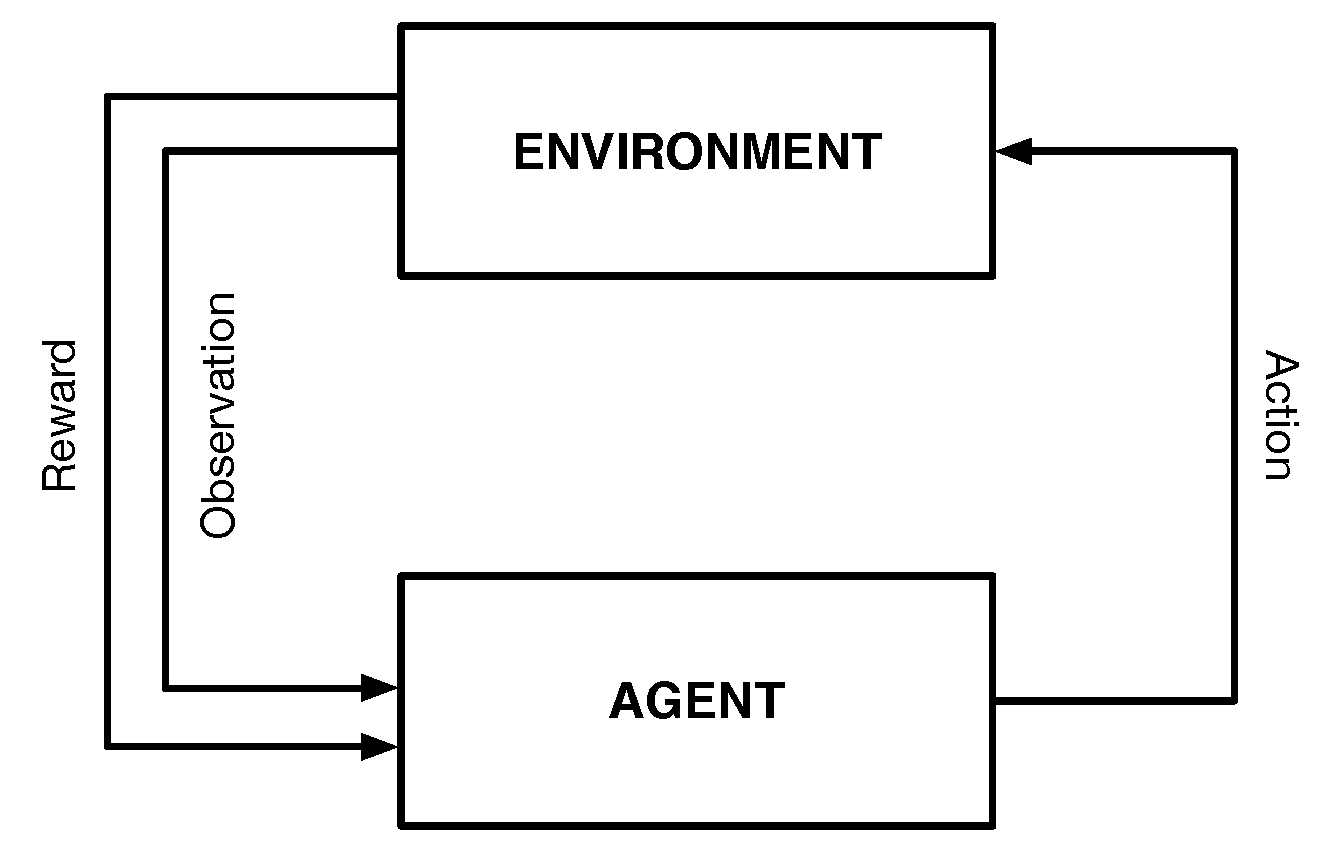
\includegraphics[width=\textwidth]{images/agent-environment.pdf}
\caption{The reinforcement learning process}
\label{fig:agentandenvironment}
\end{figure}
After the action is taken, the state of the environment changes and the agent then receives a new observation of it, and then the process repeats.  The goal of the reinforcement learning agent is to maximize the reward received over a certain time period, finding a balance between immediate and future rewards. 
\end{comment}

Reinforcement learning is an approach to the learning from experience problem in artificial intelligence. A reinforcement learning algorithm's intelligence is built upon having experiences which are then incorporated into the algorithm's own domain knowledge. This knowledge is then used to make intelligent decisions in the future \parencite{barto1998reinforcement}.

\begin{figure}[H]
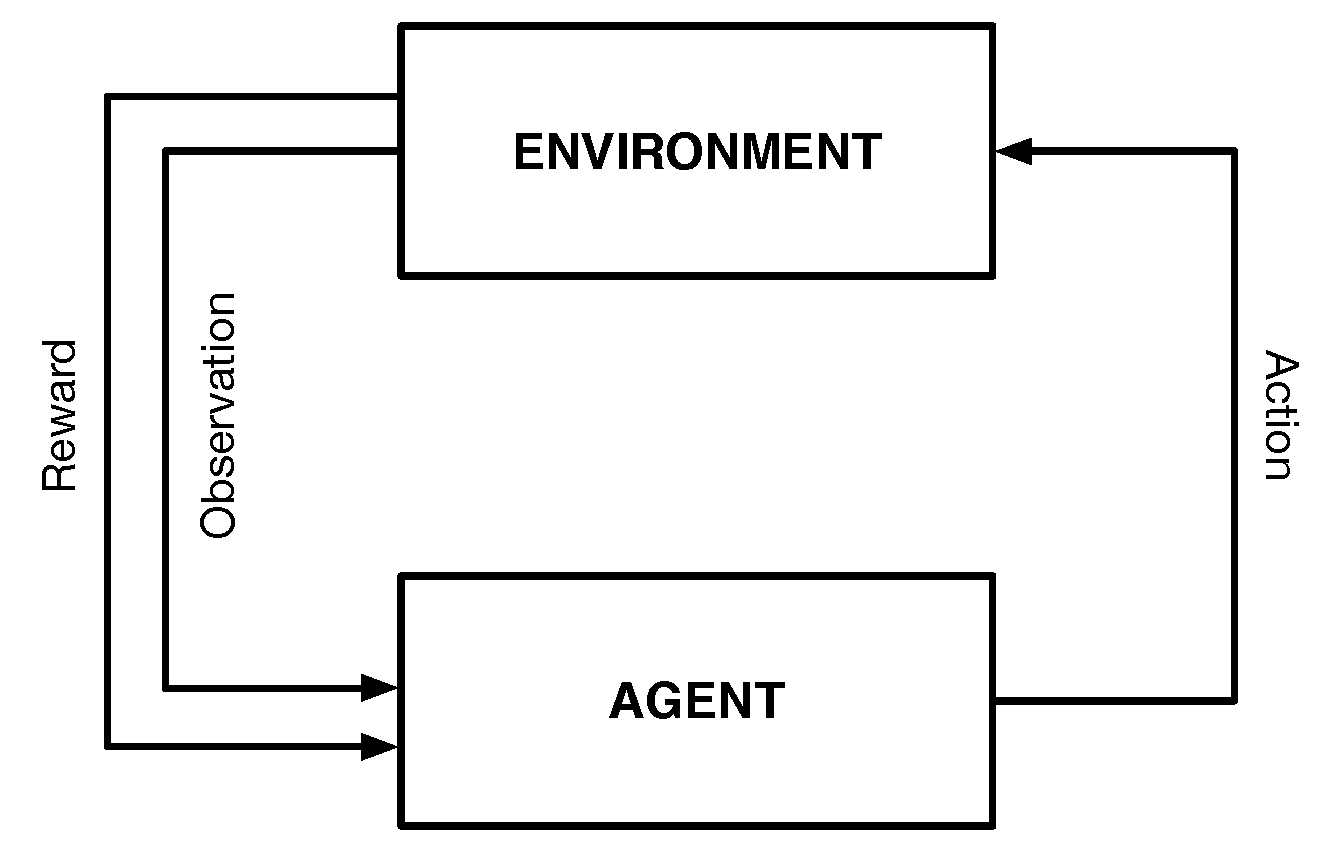
\includegraphics[width=\textwidth]{images/agent-environment.pdf}
\caption{The reinforcement learning process}
\label{fig:agentandenvironment}
\end{figure}

The reinforcement learning problem is modeled as a sequential decision problem, see figure \ref{fig:agentandenvironment} for a graphical representation of the process. A learning algorithm, an agent, performs an action and receives a reward according to some measure of how desirable the results of the action are.  After the action is taken, the state of the environment changes and the agent then receives a new observation of it, and then the process repeats. The goal of the reinforcement learning agent is to maximize the reward received over a certain time period, finding a balance between immediate and future rewards \parencite{barto1998reinforcement}. 


%One thing that sets reinforcement learning apart from other fields within artificial intelligence is that a reinforcement learning problem is solved by an online algorithm. That is, a reinforcement learning algorithm learns about its task and environment while operating in the environment. The actions taken by the agent affect what it knows about the environment, and thus its appraisal of the value of future actions and/or states of the environment.


There are several ways of further dividing reinforcement learning problems into other subcategories. Some examples are the dichotomies 1) episodic/non-episodic problems 2) problems with continuous/discrete state spaces 3) problems with continuous/discrete action spaces 4) problems with one/multiple concurrent agents. (etc.) In the text below, the two first of these dichotomies, which are relevant to this thesis, are discussed. 

\subsection{Episodic and Non-episodic Problems}
One can categorize reinforcement learning problems based on whether or not the time steps are divided into episodes. When the time steps for the agent-environment interaction are divided into subsequences in this manner, the problem is called episodic. This is common in for example games, which end when they are won or lost. If the problem is not episodic, it is called non-episodic, which means, consequently, that the interaction is not divided into subsequences. Instead, the interaction between the actor and environment goes on continually without end \parencite{barto1998reinforcement}. Two examples of non-episodic applications are controlling a robot arm (as well as other robotics problems) and maneuvering a helicopter \parencite{ng2006autonomous}. 

\subsection{Continuous and Discrete Problems}
An alternative way to categorize reinforcement learning problems is based on whether their state spaces are continuous or discrete. An important difference between the two kinds of problems is how an agent can treat similar states in the model. In a continuous problem it is a lot easier to group together states located around the same ``position'' due to the nature of a continuous problem, where the states usually more or less meld together. For example, if the reinforcement learning problem is to control a robot arm whose position is the state of the environment, the different states located around the same general area are not very different. This means that they might be treated in the same way or a similar way by an agent. On the other hand, consider the discrete problem of a game of connect four, wherein the placement of a coin into one of two adjacent slots could dramatically change the evaluation of the state and the outcome of the game \parencite{barto1998reinforcement}.

psection{Markov decision process}

Within reinforcement learning, the concept of Markov secision processes (MDP) is central. An MDP is a way to model an environment where state changes in it are dependent on both random chance and the actions of an agent. An MDP is defined by the quadruple $\left( S, A, P( \cdot , \cdot, \cdot ) , R( \cdot , \cdot ) \right)$ \parencite{altman2002applications}: 

\begin{description}
\item[$S$] \hfill \\ 
    A set of states representing the environment.
\item[$A$] \hfill \\ 
    A set of actions that can be taken.
\item[$P \colon S \times A \times S \to \mathbb R$] \hfill \\ 
    A probability distribution over the transitions in the environment. This function describes the probability of ending up in a certain target state when a certain action is taken from a certain origin state. 
\item[$R \colon S \times A \to \mathbb{R}$] \hfill \\ 
    A function for the reward associated with a state transition. In some formulation of MDPs the reward function only depends on the state.
\end{description}

MDPs are similar to Markov chains, but there are two differences. First, there is a concept of rewards in MDPs, which is absent in Markov chains. Second, in a Markov chain, the only thing that affects the probabilities of transitioning to other states is the current state, whereas in an MPD both the current state and the action taken in that state are needed to know the probability distribution connected with the next state \parencite{altman2002applications}.


\input{Technical_Background/MDP/markov_property.tex}
\input{Technical_Background/MDP/sparse_mdps.tex}
\input{Technical_Background/MDP/factored_representations.tex}


\section{Basic algorithms for solving MDPs}

A policy $\pi$ is a function from a state $s$ to an action $a$ that operates in
the context of a Markov Decision Process, i.e. $\pi \colon S \to A$. A policy
is thus a description of how to act in each state of an MDP. An arbitrary
policy is denoted by $\pi$ and the optimal policy (the policy with the largest
expected reward in the MDP) is denoted by $*$. The rest of this section is
describes some basic algorithms for solving, that is to say finding an optimal
policy, in an MDP.

\subsection{Value functions}

To solve an MDP most algorithms uses an estimation of values of states or
actions. Two value functions are usually defined, the state-value function $V :
S \to \mathbb R$ and the state-action-value function $Q : S \times A \to
\mathbb R$. As the names implies $V$ signifies how good a state is, while $Q$
signifies how good an action in a state is. The state-value function,
$V^\pi(s)$, returns the expected value when starting in state $s$ and following
policy $\pi$ thereafter. Equations \eqref{equation:v_finite} and \eqref{equation:v_infinite} show the equations for the state-value function for a finite time horizon and an infinite, discounted, time horizon respectively. In \eqref{equation:v_infinite}, $\gamma$ is the discount factor, a value between 0 and 1 which describes how fast the value of expected future rewards decay as one looks further into the future. The state-action-value function $Q^\pi(s, a)$ returns
the expected value when starting in state $s$ and taking action $a$ and
thereafter following policy $\pi$. The value functions for the optimal policy
are denoted by $V^*(s)$ and $Q^*(s, a)$. Formulas for the state-action value functions are anologous to those presented for the state value functions. 

\begin{align}
\label{equation:v_finite}
V_t^\pi(s) = \mathbb{E} \{ \sum_{k=0}^{T=k} r_{t+k} | S_t = S, \pi \}
\end{align}

\begin{align}
\label{equation:v_infinite}
V_{0}^\pi(s) = \mathbb{E} \{ \sum_{t=0}^\infty r_{t}\gamma^t | S_0 = S,\pi \}
\end{align}

Both $V^\pi$ and $Q^\pi$ can be estimated from experience. This can be done by
maintaining the average of the rewards that have followed each state when
following the policy $\pi$. When the number of times the state has been
encountered goes to infinity, the average over these histories of rewards
converges to the true values of the value function
\parencite{barto1998reinforcement}.

\input{Technical_Background/ValueFunctions/dynamic_programming.tex}
\input{Technical_Background/ValueFunctions/policy_iteration.tex}
\input{Technical_Background/ValueFunctions/value_iteration.tex}


\subsection{\etre\ in Factored Markov Decision Processes 
\note{N}}
\label{sec:e3_factored_discussion}

\paragraph{General shape of the results} In a comparison of the \etre\ agent's behavior in the different-size environments, the similarity of the shape of the graphs is striking. At first there is a period of lower and lower performance. (For the smallest environments, this period is very short, however.) Next, there is a period of fairly constant high performance, which lasts until the end of the experiment.  

This shape can be explained as a consequence of the different phases of operation of the \etre\ algorithm coupled with the structure of the MDP studied. In the beginning of the experiment, the algorithm will spend almost all of its time in the balanced wandering and exploration phases. The longer the agent has been exploring, and the more states become known, the further the agent has to explore into hard-to-reach parts of the MDP to find unexplored states. Now, in the case of the invasive species environment with the parameters chosen as in the experiments presented, the most easily reachable states are the ones where there is no tamarisk infection. This means that the harder a state is to reach, the more infected it will be, and thus the performance of the \etre\ agent in the exploration phase will fall as the experiment progresses. 

However, once the agent knows enough about the environment to enter the exploitation phase, the \etre\ agent spends close to no time at all exploring unknown states, and it retains high performance. 

\paragraph{Consequences of pooling observation data} An interesting result is that the agent is able to enter the exploitation phase for the 10 reaches/1 habitat per reach test setup slightly earlier than for the 5 reaches/1 habitat per reach setup. This is probably connected to the optimization described in the last paragraph of section \ref{sec:factored_e3}. In the 10 reaches/1 habitat per reach case there are nine reaches with two parents (including the reach itself) and one reach with only itself as parent. In the 5 reaches/1 habitat per reach case there are four reaches with two parents and one reach with only itself as parent. Since observations for state variables with similar parent structure are pooled by our \etre\ implementation, the agent will receive almost double the information per time step for the two-parent reaches in the 10 reaches case as compared to the 5 reaches case.  

\paragraph{Possible issues with the one-policy-per-reach optimization} In section \ref{sec:one_policy_per_state_variable} an optimization is described that works very well for the particular environment and environment settings that the agent was tested for. However, this optimization makes several assumptions that may cause problems if the settings are changed. For instance, one assumption is that the state of a reach is only affected directly by its adjacent parents in the DBN. If the state of a reach was made to depend significantly on other reaches two or more levels up in the river network, the agent would probably not be able to converge on an optimal policy. 

Another assumption that could lead to problems with other environment settings is the assumption that the maximal action cost in the environment is impossible or very hard to break. The invasive species environment has a maximum cost for actions. However, with the standard settings it is mathematically impossible to break this maximum. Our implementation of \etre\ would achieve very poor performance if this was not the case, since a large penalty is given when the maximum action cost is breached. 

\paragraph{DBN structure} Finally, in the invasive species environment, the structure of the DBN underlying the MDP is known at the start of the experiment, so the agent does not need to infer it from its observations. If this was not the case, all the DBN optimizations would be useless unless some kind of algorithm for infering the DBN structure was added to the agent. 

\chapter{Environment and algorithms}
\label{ch:algo}

This chapter gives a description of the environment and the algorithms that
were used in the experiment described in chapter \ref{ch:method}. The environment Invasive Species, is a simulation of a river network with invading species where to goal is to eradicate unwanted species and is further described in section \ref{sec:experiment_env}. 

Two algorithms are covered in this chapter, both of which deal with the
problems that arise with large state spaces; however, they differ in the
methods they apply. In the following chapter the general ideas behind the
algorithms, as well as specific details, are presented. 

The model-based interval estimation algorithm, described in
section~\ref{sec:mbie}, utilizes clever estimations of confidence intervals for
the Q-value functions to improve performance in sparse MDPs.
Section~\ref{sec:fac_e3} is on an algorithm that uses dynamic bayesian networks
and factored representations to improve the \etre\ algorithm to efficiently
deal with factored MDPs. 

\section{Environment specification, Invasive Species}
\label{sec:experiment_env}

When the agents were tested, the Invasive Species environment from the 2014 edition of
the Reinforcement Learning Competition was used. The environment is a
simulation of an invasive species problem, in this case a river network with
invading species where the goal of the agent is to eradicate unwanted species
while replanting native species. 

The environment's model of the river network has parameters, such as the size
of the river network and the rate at which plants spread, which can be
configured in order to create different variations of the environment.  The
size of the river network is defined by two parameters: the number of reaches
and the number of habitats per reach. A habitat is the smallest unit of land
that is considered in the problem. A habitat can either be invaded by the
tamarix, which is an unwanted species, empty or occupied by native species. A
reach is a collection of neighboring habitats. The structure of the river
network is defined in terms of which reach is connected to which
\parencite{invasiveSpecis2014:Online}. In figure \ref{fig:river} a model of a
river network is shown.

\begin{figure}[ht]
\centering
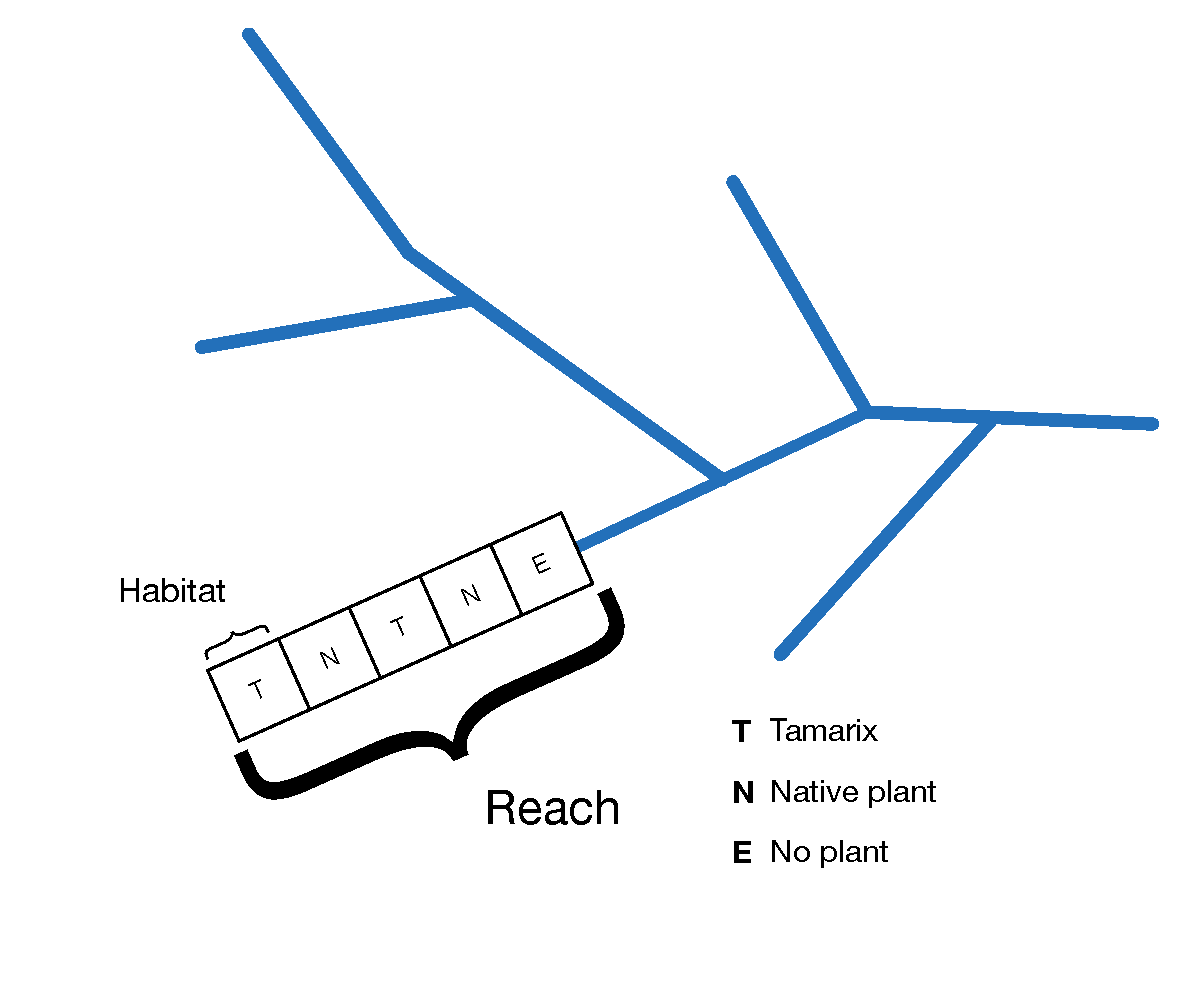
\includegraphics[width=0.9\textwidth]{images/river_network.pdf}
\caption{A river network, as modeled by the Invasive Species reinforcement learning environment.}
\label{fig:river}
\end{figure}

There are four possible actions (eradicate tamarix trees, plant native trees,
eradicate tamarix trees and plant native trees and a wait-and-see action),
and the agent chooses one of these actions for each reach and time step. If the 
agent chooses to eradicate tamarix trees or plant native trees in a reach, 
all habitats of that reach are targeted by this action. What
actions are available to the agent depends on the state of each reach. It is
always possible to choose the wait-and-see action, but there has to be one
or more tamarix-invaded habitats in a reach for the eradicate or eradicate and
plant actions to be available and there has to be at least one empty habitat in
a reach for the plant-native-trees action to be available
\parencite{invasiveSpecis2014:Online}.  

\section{Model-based interval estimation}
\label{sec:mbie}

Model-based interval estimation is a modification of value iteration whose main feature is its  addition of confidence
intervals to the state-action values. These confidence intervals allow the agent to choose between
actions, based on how confident it is about its evaluation of them. In effect,
the less certain the agent is about its evaluation of the states and actions,
the more exploratory the actions will be. When the agent is more confident
however, it will exploit what it has learnt so far about the MDP
\parencite{dietterich2013pac}.

\input{algorithms/MBIE/modification_of_value_it}
\input{algorithms/MBIE/gt.tex}
\input{algorithms/MBIE/modded_bounds}

\section{\etre\ in factored Markov decision processes}
\label{sec:fac_e3}

The second algorithm studied in this thesis is a version of the \etre\ algorithm that focuses on factored problem domains by modeling them as a dynamic Bayesian network. The original \etre\ algorithm is described in section \ref{sec:e3}, which gives a broad overview along with the key strategies used in the algorithm. The following section, \ref{sec:factored_e3}, considers some ways to extend the original algorithm and make use of factored representations and planning in factored domains to improve the running time of the algorithm.

\input{algorithms/Factored_E3/e3.tex}
\input{algorithms/Factored_E3/factored_additions.tex}


\chapter{Method}
\label{sec:method_intro}

This chapter covers the preliminaries and preparations carried out before the
execution of the experiments. It covers  and how the agents described in chapter
\ref{ch:algo} were implemented and the additions and modifications that were made to them. The chapter
concludes with a description of the tools used for the experiment.
\section{Algorithm implementation}
\label{sec:implementation}

We implemented two existing algorithms and we also added some extensions.  The
experiment utilized RL-Glue (section~\ref{sec:rl_glue}) to connect the agents
and environment to each other.  To verify the behavior of our agents we utilized smaller
environments (see sections~\ref{sec:intro_grid_world} and \ref{sec:ns}) where
the correct operation is either easy to derive or obvious from inspection. By
starting with smaller problems and using an iterative approach it was possible
to identify bottlenecks in our implementations and correct possible errors
early.

\input{algorithms/MBIE/modded_bounds}

\input{method/ConstructingExperiments/contributionse3}

\subsection{GridWorld}
\label{sec:intro_grid_world}

The GridWorld environment was implemented to easily be able to verify the
correctness of the MBIE algorithm. It consists of a grid of twelve squares with
one blocked square, one starting square, one winning square, one losing square and
eight empty squares. The agent can take five actions, north, south, west,
east or exit. The exit-action is only possible from the winning or losing
state. When taking an action being in one state and the action is directed to
another empty state there is an 80\% probability to succeed and 10\%
probability to fail and 10\% to go sideways.

\subsection{Network simulator}
\label{sec:ns}

A simple computer network simulation was implemented to verify the behavior of an
early version of \etre\ algorithm. In this environment, the agent tries to keep
a network of computers up and running. All computers start in the running
state, but there is a chance that they randomly stop working. If a computer is
down, it has a chance to cause other computers connected to it to also fail. In
each time step, the agent chooses one computer to restart, which with 100
percent probability will be in working condition in the next time step. The
agent is rewarded for each computer in the running state after each time step. 

\section{Our contributions}
\label{sec:contributions}


\input{algorithms/MBIE/modded_bounds}


\input{method/ConstructingExperiments/contributionse3}

\section{Environment specification}
\label{sec:experiment_env}

For the experiment, the Invasive Species environment from the 2014 edition of
the Reinforcement Learning Competition was used. The environment is a
simulation of an invasive species problem, in this case a river network with
invading species where the goal of the agent is to eradicate unwanted species
while replanting native species. 

The environment's model of the river network has parameters, such as the size
of the river network and the rate at which plants spread, which can be
configured in order to create different variations of the environment.  The
size of the river network is defined by two parameters: the number of reaches
and the number of habitats per reach. A habitat is the smallest unit of land
that is considered in the problem. A habitat can either be invaded by the
tamarix, which is an unwanted species, empty or occupied by native species. A
reach is a collection of neighboring habitats. The structure of the river
network is defined in terms of which reach is connected to which
\parencite{invasiveSpecis2014:Online}. In figure \ref{fig:river} a model of a
river network is shown.

\begin{figure}[ht]
\centering
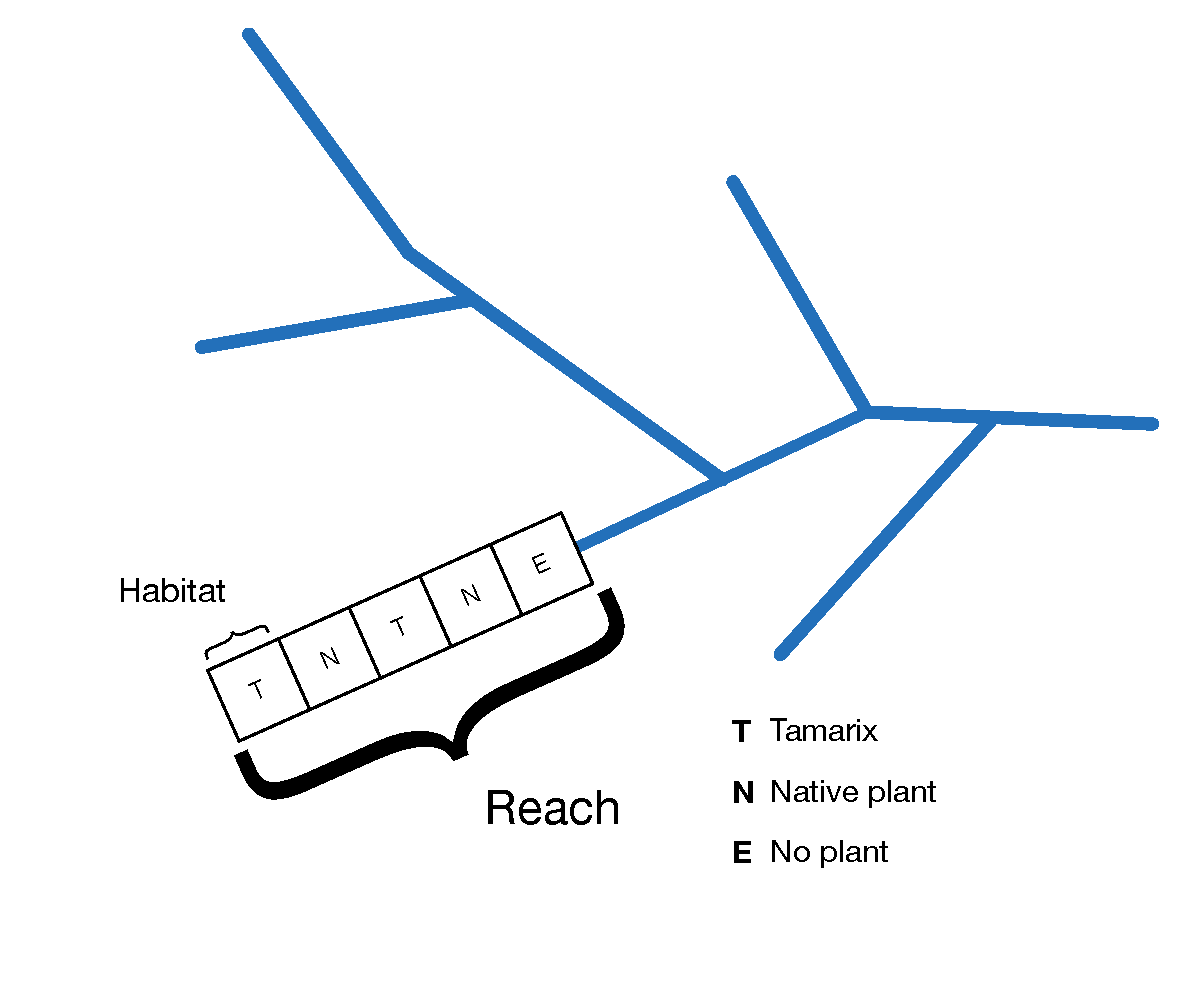
\includegraphics[width=0.9\textwidth]{images/river_network.pdf}
\caption{A river network, as modelled by the Invasive Species reinforcement learning environment.}
\label{fig:river}
\end{figure}

There are four possible actions (eradicate tamarisks, plant native trees,
eradicate tamarisks and plant native trees, and finally a wait-and-see action),
and the agent chooses one of these actions per reach per time step. What
actions are available to the agent depends on the state of each reach. It is
always possible to choose the wait-and-see action, but there has to be one
or more tamarix-invaded habitats in a reach for the eradicate or eradicate and
plant actions to be available and there has to be at least one empty habitat in
a reach for the plant-native-trees action to be avalable
\parencite{invasiveSpecis2014:Online}. 

\section{Test specification}
\label{sec:test_spec}

The testing of the agents required us to choose certain sets of parameters, for
the environment, the two different agents and the experiment itself. 

\paragraph{Environment parameters}

The Invasive Species environment requires a number of parameters. For further
explanation of the environment parameters consult the environment
webpage\footnote{\url{http://2013.rl-competition.org/domains/invasive-species}}.
The specific parameters used are presented in
appendix~\ref{ap:environment_spec}.

\paragraph{Agent Parameters}

The agents evaluated required different types of parameters. Some preliminary
tests were run and then the parameters giving best results were chosen.
Parameters for MBIE are found in table~\ref{tab:mbie_params_both}.

\begin{table}[H]
\centering
\captionof{table}{Parameters for MBIE}
\label{tab:mbie_params_both}

\begin{subfigure}[b]{0.47\textwidth}
    \centering
    \captionof{table}{Proper MBIE}
    \label{tab:mbie_params} 
    \begin{tabular}{lr}
     \toprule
     Parameter & Value \\
     \midrule
     Discount factor, $\gamma$ & 0.9 \\
     Confidence, $\delta$ & 95\% \\
     $\Delta \omega$ & $\frac{1}{2}\sqrt{\frac{2|ln(2^{|S|}-2) - ln  \delta |}{N(s,a)}}$ \\
     
     \bottomrule
    \end{tabular}
\end{subfigure}
\quad
\begin{subfigure}[b]{0.47\textwidth}
    \centering
    \captionof{table}{Realistic MBIE}
    \label{tab:mbie_realistic_params}
    \begin{tabular}{lr}
     \toprule
     Parameter & Value \\
     \midrule
     Discount factor, $\gamma$ & 0.9 \\
     $\Delta \omega$ & $1 - 0.05 N(s,a)$ \\
     \bottomrule
    \end{tabular}
\end{subfigure}
\end{table}

For DBN-\etre\ a higher exploration limit resulted in the agent starting to
exploit earlier but with a slightly lower final return. A higher partial state
known limit resulted in later exploitation but no appreciable difference in
final return. The values in table~\ref{tab:dbne3_params} were a good middle
ground.

\begin{table}[H]
\captionof{table}{DBN-\etre\ parameters}
\label{tab:dbne3_params}
\centering
\begin{tabular}{lr}
 \toprule
 Parameter & Value \\
 \midrule
 Discount factor & 0.9 \\
 Exploration limit & 5\% \\
 Partial state known limit & 5 \\
 \bottomrule
\end{tabular}
\end{table}

\paragraph{Experiment parameters}

The tests performed had to be long enough to sample enough data to extract
relevant results without making the running time too long. A single test
consisted of a specific number of episodes with a specific length. A good
combination was required to efficiently evaluate the agents. If a single
episode consisted of too many samples it would be difficult to see the learning
process as results are reported as total reward over an episode and that
process might be hidden as its impact on the total reward is smaller with a
longer episode. On the other hand, if an episode length is too short it would
end before the agents could do any valuable learning.

In addition to a satisfactory episode length, a reasonable number of episodes
needs to be sampled for it to be possible to draw conclusions from the results.
If the number of episodes is too small, the convergence of the agents cannot be
seen. However, if the number of episodes are too large a lot of sampled data
would be redundant for the study. Some preliminary experiments were run in
order to tune the experiment parameters to suitable values. The episode length
was set to 100 samples and there were 100 episodes per test.

To evaluate the agents in the Invasive Species environment combinations of
reaches and number of habitats per reach that can be seen in
table~\ref{tab:reaches_habitats} were choosen. Combinations were chosen to have
a wide range in the total number of states for the agents to deal with and to
test how the agents deal with taking actions that have to take into account
several state components. 

As seen in table ~\ref{tab:reaches_habitats}, the state count increases rapidly
when habitats are added to the problem. This is obvious from the fact that the state count
depends exponentially on the total number of habitats; see equation \eqref{eq:statecount}, where $h$ is the number of habitats per reach and $r$ is the number of reaches.

\begin{equation}
\label{eq:statecount}
 |S| = 3 ^ {hr}
\end{equation}

\begin{table}[H]
\centering
\caption{Combinations of reaches and habitats used in testing.}
\label{tab:reaches_habitats}
\begin{tabular}{rrr}
 \toprule
 Reaches & Habitats per reach & Total state count \\
 \midrule
 5  & 1 &          243 \\
 3  & 2 &          729 \\
 3  & 3 &      19\,683 \\
 10 & 1 &      59\,049 \\
 4  & 3 &     531\,441 \\
 5  & 3 & 14\,348\,907 \\
 \bottomrule
\end{tabular}
\end{table}

\section{Programming environment}
\label{sec:prog_env}

The Java programming language 1.7 was used to implement the algorithms. In addition, the
Java version of RL-Glue framework version 3.0 was used. For version control Git
was used, due to its simplicity and performance.

\section{RL-Glue}
\label{sec:rl_glue}

To evaluate the agents the RL-Glue framework was used, which acts as an
interface for communication between the agent and the environment. The software
uses the RL-Glue protocol, which specifies how a reinforcement learning problem
should be divided when constructing experiments and how the different programs
should communicate \parencite{tanner2009rl}.

RL-Glue divides the reinforcement learning process into three separate
programs: an agent, an environment and an experiment. RL-Glue provides a server
software that manages the communication between these programs. The agent and
the environment programs are responsible for executing the tasks as specified
by RL-Glue and the experiment program acts as a bridge between the agent and
environment \parencite{tanner2009rl}.

The modular structure of RL-Glue makes it easier to construct repeatable
reinforcement learning experiments. By separating the agent from the
environment it is possible to reuse the environment and switch out the agent.
It also makes it a lot easier to cooperate and continue working on existing
environments implemented by other programmers.


\chapter{Result}

\newcommand{\graphwidth}{0.70\textwidth}
\newcommand{\testsubfigure}[2]{%
\begin{subfigure}[b]{\graphwidth}
    \includegraphics[width=1.1\textwidth]{images/tests/#1r-#2h.pdf}
    \caption{#1 reaches and #2 habitats per reach}
    \label{fig:#1r#2h}
\end{subfigure}
}

In figures~\ref{fig:tests1}, \ref{fig:tests2} and \ref{fig:tests3} we have test results from running our agents on the invasive species environment on different sizes of river network. The raw data can be found in appendix~\ref{ap:result_tables}.

\begin{figure}[h!]
    \centerline{
    \testsubfigure{3}{3}
    ~
    \testsubfigure{3}{2}
    }
    \caption{Test runs with different number of reaches and habitats}
    \label{fig:tests1}
\end{figure}

\begin{figure}[h!]
    \centerline{
    \testsubfigure{5}{1}
    ~
    \testsubfigure{5}{3}
    }
    \caption{Test runs with different number of reaches and habitats}
    \label{fig:tests2}
\end{figure}

\begin{figure}[h!]
    \centerline{
    \testsubfigure{4}{3}
    ~
    \testsubfigure{10}{1}
    }
    \caption{Test runs with different number of reaches and habitats}
    \label{fig:tests3}
\end{figure}

The agent learns for 100 episodes with 100 samples per episode, other parameters are specified in section~\ref{sec:test_spec}. The invasive species environment associates a certain cost with each state and action, thus the reward is always negative. In each test the reward varies over time for the MBIE agent, the realistic MBIE agent and the DBN-\etre\ agent.

With smaller state spaces (see figure~\ref{fig:3r3h}, \ref{fig:3r2h} and \ref{fig:5r1h}) we can see that the realistic MBIE agent outperforms the proper MBIE agent and comes close to the DBN-\etre\ agent. In the tests where the state space is larger (see figure~\ref{fig:5r3h}, \ref{fig:10r1h} and \ref{fig:4r3h}) proper MBIE and realistic MBIE are very close to each other in performance while the DBN-\etre\ agent outperforms both. The realistic MBIE algorithm performs better in with smaller state spaces due to more states becoming known quicker and thus having their true value.

In each of the test runs the DBN-\etre\ algorithm exhibits a period of learning that corresponds to exploration (as described in section~\ref{sec:e3}) where the agent has not explored the environment enough and seeks more information. This is apparent in figure~\ref{fig:3r3h}.
\chapter{Discussion \note{B}}
\label{ch:discussion}
This chapter is a discussion of the results and method used in the project. The algorithms are evaluated with regard to their performance achieved in the tests, which is used as a basis when comparing them against each-other. Determining their strengths and weaknesses and if they were suitable for problems with an environment that has a large discrete state space and in particular for the environment Invasive Species. There is also a discussion on ethical aspects regarding the work in this thesis.


% Det behövs inte en ingående disposition här, det tar ner läsligheten. Det som tas upp i styckena är vettigt, men detta är inte rätt ställe för dem.

% This chapter is a combination of discussion of the results of using the algorithms described in chapter \ref{ch:algo}, together with a examination of the method used in the project. The algorithms is evaluated with regard to their performance achieved in the experiments \ref{sec:constructing_experiments}, which is used for a basis when comparing them against each-other. Focusing on their strengths and weaknesses and circling around the question why did they perform as they did. Were they suitable for this kind of problem, an environment with a large discrete state space and in particular for this thesis a simulation of an Invasive Species environment.

% The second part of this chapter contains a section containing a presentation of similar studies conducted, summarizing their results and opinions. Using their finding as a basis, there will also be a discussion regarding its connection to the results in this thesis. With inspiration from similar studies in combination with the results of this thesis, a discussion about the possible extensions and additional work or unanswered questions in this thesis are presented. 

%In order to round of this chapter, the last section of this chapter revolves around ethical questions and aspects regarding the theme of this topic. The main theme of the last section is ethical aspects in \acrlong{ai} \acrshort{ai}, \acrfull{ai}, along with a discussion about the usefulness of Reinforcement Learning in today's society with focus on using simulations.

\section{Evaluation of the agents \note{I}}
\label{sec:coa}

\input{Discussion/AlgorithmsEvaluation/dbn.tex}
\input{Discussion/AlgorithmsEvaluation/mbie.tex}
\input{Discussion/AlgorithmsEvaluation/discussion_diffrences}




\section{Potential factors impacting the results}
\label{sec:truth_results}

There are several factors that possibly reduce the reliability of the results. For instance, all evaluations used only one environment, the implementation of the algorithms could contain errors and the correct results for all test runs are not always known. 

\input{Discussion/discussion_results/impact_of_one_env.tex}

\input{Discussion/discussion_results/implementation_of_algorithms.tex}

\input{Discussion/discussion_results/testing_methodology.tex}


%\section{Similar Studies \note{N, K}}
The work with reducing the complexity of the reinforcement learning problems with environments containing large state spaces is not a new research topic. However, this thesis is taking a rather uncommon approach to the problem. Instead of trying to derive new algorithms for solving the problem, the focus is instead focused on usefulness of research conducted within the area of reinforcement learning problems. To be even more specific this thesis has zoomed in on two possible attempts on solving the problem with environments containing large state spaces. An approach that is rather uncommon and thus similar studies is as well uncommon. 
%Behöver skrivas om, tydligare
Thereby this section will combining focus on both studies similar to this thesis comparing the usefulness of research already conducted along with a summarized study of studies of work being done to reduce the complexity of environments with large state spaces.

\todo[inline]{Samma miljö kanske, dess pac?}

\paragraph{Similar Studies Regarding Comparing Existing Research}
\todo[inline]{Borde finnas återkoppling i diskussion kring detta}
It has been shown in Strehl and Littman (2004; 2008) that MBIE outperforms \etre\ in the MDPs RiverSwim and SixArms. \parencite{dietterich2013pac}


\paragraph{Large State Spaces using Dynamic Bayesian Networks}
This paragraph is devoted to similar methods using dynamic Bayesian networks as an underlying representation in order to model the structure of the environment. Due to the relevance of using dynamic Bayesian network as a method for tackling similar problems it is thesis on its own in order to summarize them all. It is also possible to study section \ref{sec:better_planing_algos} for further references, however their main focus on the planning algorithm.

An algorithm to DBN-\etre\ is the algorithm by \textcite{ross2012model} which is as well utilizing a factored representation for the underlying structure. However, in the DBN-\etre\ algorithm no planning algorithm was specified and therefore leaving an empty square in the implementation affecting the overall complexity of the algorithm. In the algorithm by \textcite{ross2012model} 

\todo[inline]{Resultatjämförelse}

\paragraph{Similar Studies Regarding Large State Spaces Using Model Based Something grejen}
Grattis MBIE, er punkt.

\section{Ethical and social aspects of artificial intelligence}

\input{Discussion/Ethics/intro.tex}

\input{Discussion/Ethics/invasive_species.tex}

\input{Discussion/Ethics/ai_right_or_wrong.tex}



\section{Further work}

In this section we discuss possible further work and extensions to our thesis.

\input{Discussion/further_work/more_test_envs.tex}
\input{Discussion/further_work/better_planning_dbn.tex}
\input{Discussion/further_work/MBIE.tex}
\input{Discussion/further_work/mbie_should_use_dbn.tex}


\printbibliography

\begin{appendices}

\chapter{Environment specification}
\label{sec:environment_spec}

\begin{table}[H]
\centering
\captionof{table}{Dynamic parameters common to both species}
\label{tab:dynamic_params_common} 
\begin{tabular}{l r}
 \toprule
 Parameter & Value \\
 \midrule
 Eradication rate & 0.85 \\
 Restoration rate & 0.65 \\
 Downstream spread rate & 0.5 \\
 Upstream spread rate & 0.1 \\
 \bottomrule
\end{tabular}
\end{table}

\begin{table}[H]
\centering
\captionof{table}{Dynamic parameters different between the species} \label{tab:dynamic_params_not_common}
\begin{tabular}{lrr}
\toprule
 Parameter & Native & Tamarisk \\
 \midrule
 Death rate & 0.2 & 0.2 \\
 Production rate & 200 & 200 \\
 Exogenous arrival\footnote{Arrival of seeds from outside the environment} & Yes & Yes \\
 Exogenous arrival probability & 0.1 & 0.1 \\
 Exogenous arrival number & 150 & 150 \\
 \bottomrule
\end{tabular}
\end{table}

\begin{table}[H]
\centering
\captionof{table}{Cost function parameters} \label{tab:cost_params} 
\begin{tabular}{lr}
 \toprule
 Parameter & Value \\
 \midrule
 Cost per invaded reach & 10 \\
 Cost per tree & 0.1 \\
 Cost per empty slot & 0.01 \\
 Eradication cost & 0.5 \\
 Restoration cost & 0.9 \\
 \bottomrule
\end{tabular}
\end{table}

\begin{table}[H]
\centering
 \captionof{table}{Variable costs depending on number of habitats affected by action}
 \begin{tabular}{lr}
 \toprule
 Parameter & Value \\
 \midrule
 Eradication cost & 0.4 \\
 Restoration cost for empty slot & 0.4 \\
 Restoration cost for invaded slot & 0.8 \\
 \bottomrule
\end{tabular}
\label{tab:cost_params_var}
\end{table}
\end{appendices}


\end{document}

\RequirePackage[l2tabu,orthodox]{nag}

\documentclass[bachelors,a4paper]{chalmers-thesis}

\usepackage[swedish, english]{babel}

\usepackage[utf8]{inputenc}
\usepackage{comment}
\usepackage{color}
\usepackage{todonotes}
\usepackage{hyperref}


% To be able to include pdfs in the document
\usepackage{pdfpages}

% To use appendices
\usepackage[toc,page]{appendix}

% Fancy maths!
\usepackage{amsmath}
\usepackage{amssymb}

% Fancy references
\usepackage[style=authoryear,date=iso8601]{biblatex}
\addbibresource{jelzin.bib}

% Fancy graphics
\usepackage{graphicx}

% For the finest tables
\usepackage{booktabs}
\usepackage{longtable}

% For mutliple column pages
\usepackage{multicol}

% For the finest of subfigures in figures or tables
\usepackage{subcaption}

% To be able to position figure envs exactly where you want them use H.
\usepackage{float}

% Nice environments for pseudocode
\usepackage[chapter]{algorithm}
\usepackage{algpseudocode}

\title{Reinforcement learning}
\subtitle{A comparison of learning agents in environments with large discrete state spaces}
\author{%
Johan Andersson\and
Emil Kristiansson\and
Joakim Persson\and
Adam Sandberg Eriksson\and
Daniel Toom\and
Joppe Widstam}
\thesisin{Computer Science}
\department{Department of Computer Science and Engineering}
\reportno{2014:05}
\copyrightyear{2014}
\keywords{Reinforcement learning, Artificial intelligence, MBIE, DBN-\etre, Invasive Species, Learning algorithms}

% Abstracts
\firstabstract{% 1 Motivation

For some real-world behavior optimization problems, it is infeasible to search for a solution by making a model of the problem and performing calculations on it. 
In cases like these, good solutions can sometimes be found by trial and error. 
Reinforcement learning is a way of finding optimal behavior by systematic trial and error.
% 2 Problem statement
This thesis aims to compare different reinforcement learning techniques and evaluate them. 
Model-based interval estimation (MBIE) and Explicit explore or exploit using dynamic bayesian networks - (DBN-\etre)
 are two algorithms that are evaluated. 
% 3 Approach
To evaluate the techniques, learning agents were constructed using the algorithms and 
then simulated in the environment invasive species from the reinforcement learning competition.
% 4 Results
The results of the study show that an optimized version of DBN-\etre\ is better than MBIE at finding an optimal or near optimal behavior policy in the 
environment invasive species for a selection of environment parameters.

% 5 Conclusions
Using a factored model like a DBN shows certain advantages operating in 
the factored environment invasive species. For example it achieves a near optimal
policy within fewer episodes than MBIE.


% Följande saker ska vara med i en abstract Motivation, Problem Statement, Approach, REsults

% Motivation
% Why do we care about the problem and the results? 
% If the problem isn't obviously "interesting" it might be better to
% put motivation first; but if your work is incremental progress on
% a problem that is widely recognized as important, then it is 
% probably better to put the problem statement first to indicate which
%  piece of the larger problem you are breaking off to work on.
% This section should include the importance of your work, the difficulty
% of the area, and the impact it might have if successful.

% Problem statement
% What problem are you trying to solve? What is the scope of your work 
%(a generalized approach, or for a specific situation)? Be careful not to 
% use too much jargon. In some cases it is appropriate to put the problem 
% statement before the motivation, but usually this only works if most 
% readers already understand why the problem is important.

% Approach
% How did you go about solving or making progress on the problem? Did you 
% use simulation, analytic models, prototype construction, or analysis of
% field data for an actual product? What was the extent of your work
% (did you look at one application program or a hundred programs in
% twenty different programming languages?) What important variables did
% you control, ignore, or measure?

% Results
% What's the answer? Specifically, most good computer architecture papers 
% conclude that something is so many percent faster, cheaper, smaller, 
% or otherwise better than something else. Put the result there, in
% numbers. Avoid vague, hand-waving results such as "very", "small",
% or "significant." If you must be vague, you are only given license
% to do so when you can talk about orders-of-magnitude improvement. 
% There is a tension here in that you should not provide numbers that
% can be easily misinterpreted, but on the other hand you don't have
% room for all the caveats.

% Conclusions
% What are the implications of your answer? Is it going to change the 
% world (unlikely), be a significant "win", be a nice hack, or simply 
% serve as a road sign indicating that this path is a waste of time 
% (all of the previous results are useful). Are your results general, 
% potentially generalizable, or specific to a particular case?
}
\secondabstract{swedish}{% 1 Motivation
För vissa verklighetsbaserade optimeringsproblem där det gäller att finna ett bästa beteende är det orimligt söka efter det optimala beteendet genom att skapa en modell av problemet och sedan utföra beräkningar på den. I vissa sådana fall kan man hitta bra lösningar genom trial and error. Reinforcement learning är ett sätt att hitta optimalt beteende genom att systematisk pröva sig fram.
% 2 Problem statement
Detta kandidatarbete har som mål att jämföra olika inlärningstekniker och utvärdera dessa.
Model-based interval estimation (MBIE) och Explicit Explore or Exploit med dynamiska bayesnät (DBN-\etre) är 
två självlärande algoritmer som här utvärderas.

% 3 Approach
För att utvärdera de olika teknikerna implementerades agenter som använde algoritmerna, och dessa testkördes sedan 
i miljön invasive species från tävlingen Reinforcement learning competition.

% 4 Results
DBN-\etre\ är bättre än MBIE på att hitta en optimal eller nära optimal policy i miljön invasive species med valda parametrar.
% 5 Conclusions
Att använda en faktoriserad model, så som DBN-\etre\, visar på tydliga fördelar i faktoriserade miljöer, som i till exempel invasive species. 
Ett exempel på detta är att den når en nästan optimal policy på färre episoder än MBIE.

% Följande saker ska vara med i en abstract Motivation, Problem Statement, Approach, REsults

% Motivation
% Why do we care about the problem and the results? 
% If the problem isn't obviously "interesting" it might be better to
% put motivation first; but if your work is incremental progress on
% a problem that is widely recognized as important, then it is 
% probably better to put the problem statement first to indicate which
%  piece of the larger problem you are breaking off to work on.
% This section should include the importance of your work, the difficulty
% of the area, and the impact it might have if successful.

% Problem statement
% What problem are you trying to solve? What is the scope of your work 
%(a generalized approach, or for a specific situation)? Be careful not to 
% use too much jargon. In some cases it is appropriate to put the problem 
% statement before the motivation, but usually this only works if most 
% readers already understand why the problem is important.

% Approach
% How did you go about solving or making progress on the problem? Did you 
% use simulation, analytic models, prototype construction, or analysis of
% field data for an actual product? What was the extent of your work
% (did you look at one application program or a hundred programs in
% twenty different programming languages?) What important variables did
% you control, ignore, or measure?

% Results
% What's the answer? Specifically, most good computer architecture papers 
% conclude that something is so many percent faster, cheaper, smaller, 
% or otherwise better than something else. Put the result there, in
% numbers. Avoid vague, hand-waving results such as "very", "small",
% or "significant." If you must be vague, you are only given license
% to do so when you can talk about orders-of-magnitude improvement. 
% There is a tension here in that you should not provide numbers that
% can be easily misinterpreted, but on the other hand you don't have
% room for all the caveats.

% Conclusions
% What are the implications of your answer? Is it going to change the 
% world (unlikely), be a significant "win", be a nice hack, or simply 
% serve as a road sign indicating that this path is a waste of time 
% (all of the previous results are useful). Are your results general, 
% potentially generalizable, or specific to a particular case?
}

% Useful commands
\newcommand{\note}[1]{\textcolor{red}{#1}}
\newcommand{\etre}{\ensuremath{E^3}}

\begin{document}

\makecoverpage
\maketitlepage
\makeprintinfopage

\newpage

\pagenumbering{roman}
\pagestyle{plain}

\makeabstractpage
\makesecondabstractpage

\newpage

\tableofcontents

\newpage

\pagenumbering{arabic}

\chapter{Introduction}
\label{sec:intro_intro}

This thesis evaluates and compares two existing algorithms and therefore it has
negliable impact on matters such as ethics, social or economics in today's
society. Therefore this sections focuses on the futher impact of artificial
intelligence using models of the real world and simulations along with a
high-level discussion regarding right or wrong with artificial intelligence.
\section{Purpose and problem statement}

This thesis aims to further the knowledge of reinforcement learning or more specifically, algorithms applied to reinforcement learning problems with large state spaces. Reinforcement learning algorithms struggle with environments consisting of large state spaces due to practical limitations in memory usage and difficulties in estimating the value of actions and states within reasonable processing time. Therefore, we aim to evaluate techniques to circumvent or reduce the impact of these limitations by implementing algorithms using these techniques and testing and comparing them on problems of different sizes.


\section{Limitations \note{Ny Text}}
\label{sec:discuss_limitations}
In section \ref{sec:limitations}, the limitations for the project were stated and besides the fact that this thesis focuses environments with large state spaces. In order for the results from testing the algorithms selected to be relevant, the choice of environment is significant. The information gathering process during the pre-study was a more complex process than expected. The clear limitation of environment phases reduced the overall complexity with the reinforcement learning field and served as a great way to narrow the field of study. Without the reduction of the potential open research areas in reinforcement learning by first selecting the problem type and a corresponding environment the project would have become significant arduous to manage and execute. 

Nevertheless, there is also a different aspect of making an early choice of environment and problem area. The early decision of environment could possibly have eliminated algorithms from other fields in reinforcement learning which could have yielded superior results than the results collected in this project. Although, given the circumstances of the project, a delay in the choice of environment only could have lead to time spent wasted and perhaps resulted in a direction of the project not leading to any significant results at all. 

Because some papers do not include proper testing, it is possible that a algorithm only works in theory due to limitations with today computers computational power and memory. Another reason behind focusing on open research topics is on the grounds that the group lacks extensive background in the reinforcement learning field and have an desire to start working with practical issues rather than spending all the time in the beginning of the project reasoning about algorithms strength and weakness first handed. Instead focusing on combining the study of reinforcement learning in general and bringing two selected agents to life, the learning outcome has been maximized and as the project matured the knowledge and understanding of the subject also matured making it easier to reason about the qualities of the algorithms and also find areas where optimizations can be applied. 
\section{Simulation environment}
\label{sec:env_used}
The environment used is invasive species from the Reinforcement Learning Competition, described in section \ref{sec:experiment_env}. Depending on the parameters, the problem can have both a large state space and/or a large action space. This makes invasive species a good choice with the given problem statement.


\section{Agents to be Evaluated}
Two algorithms that are suitable to the purpose and problem statement, since they apply different techniques for working with large state spaces, are Explicit Explore or Exploit in Dynamic Bayesian Networks (DBN-\etre) and Model Based Interval Estimation (MBIE). They are described in detail in chapter \ref{ch:algo}. 





% tests using these algorithms should yield interesting data to be used for the evaluating the two agents and compare them against each-other. 
\chapter{Technical background}
This chapter is for readers new to the reinforcement learning area. A short overview is first given of artificial intelligence and how reinforcement learning fits within the field of artificial intelligence, the chapter then continues with the main topics and concepts necessary to understand the rest of the report. 

% This technical background has a theoretical outlook and in some cases discusses the mathematical background.

%This technical background has a slightly more theoretical outlook and in some cases discusses more of the mathematical background than the introduction given in chapter \ref{sec:intro_intro}. 

The term artificial intelligence was coined by John McCarthy who described it as ``the science and engineering of making intelligent machines'' \parencite{McCarthy2007:Online}. More specifically, it addresses creating intelligent computer machines or software that can achieve specified goals computationally. These goals can comprise anything, e.g. writing poetry, playing complex games such as chess or diagnosing diseases. Different branches of artificial intelligence include planning, reasoning, pattern recognition and the focus of this thesis: learning from experience.
This chapter gives a more formal description of reinforcement learning and the main topics and concepts necessary to understand the rest of the report. 


\section{Reinforcement Learning \note{Reviderad}}

%These areas comprise different subcategories and problems of their own. An approach to learning from experience is Reinforcement Learning, where the agent takes an action and receives a reward according to some measure of how good the action was. This could be compared to Pavlovian conditioning: teaching dogs by rewarding them for desired behavior and punishing them for undesired behavior. 

\begin{comment}
Reinforcement learning is an approach to the learning from experience problem in artificial intelligence. The reinforcement learning problem is modeled as a sequential decision problem: a learning algorithm, an agent, performs an action and receives a reward according to some measure of how desirable the results of the action are. See figure \ref{fig:agentandenvironment} for a graphical representation of the process \parencite{barto1998reinforcement}.
\begin{figure}[H]
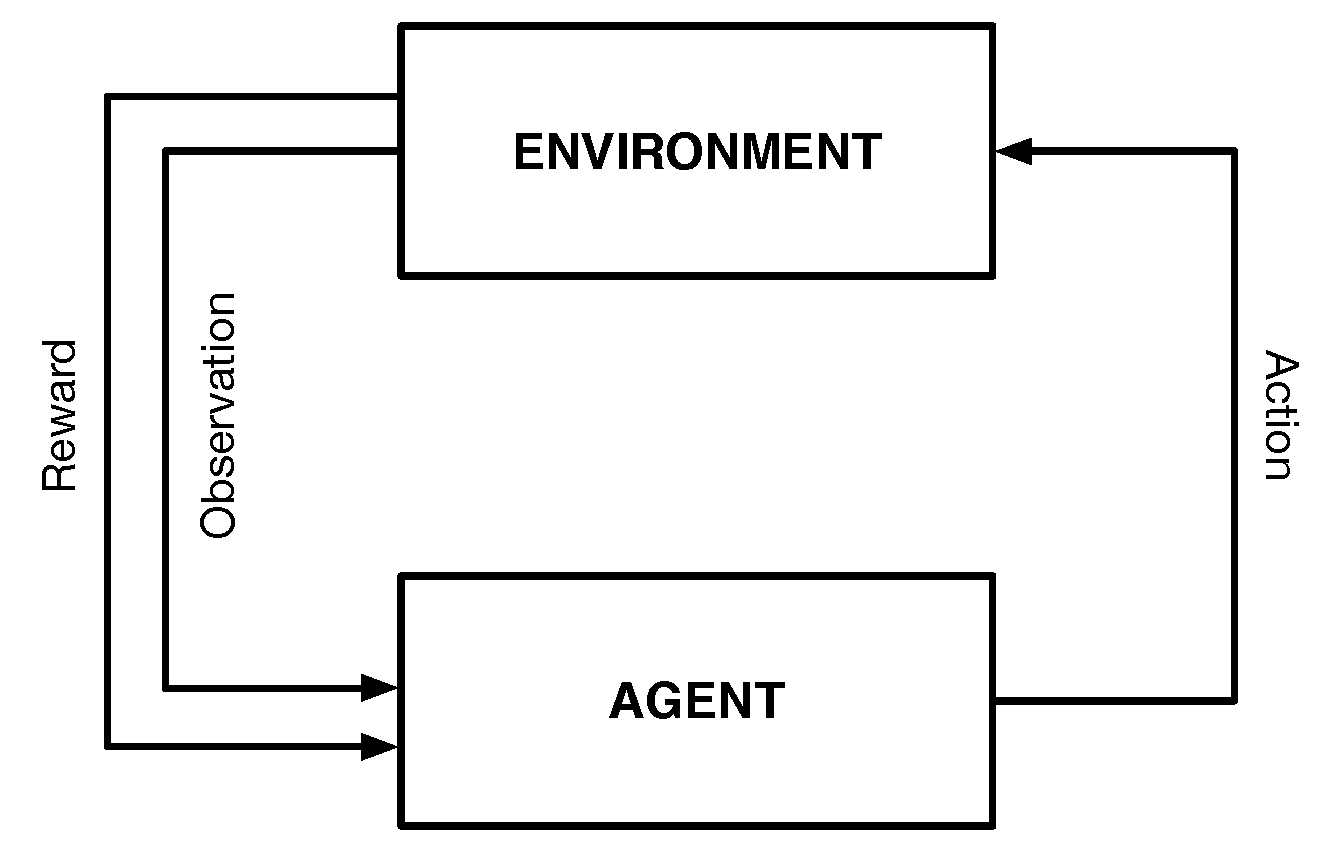
\includegraphics[width=\textwidth]{images/agent-environment.pdf}
\caption{The reinforcement learning process}
\label{fig:agentandenvironment}
\end{figure}
After the action is taken, the state of the environment changes and the agent then receives a new observation of it, and then the process repeats.  The goal of the reinforcement learning agent is to maximize the reward received over a certain time period, finding a balance between immediate and future rewards. 
\end{comment}

Reinforcement learning is an approach to the learning from experience problem in artificial intelligence. A reinforcement learning algorithm's intelligence is built upon having experiences which are then incorporated into the algorithm's own domain knowledge. This knowledge is then used to make intelligent decisions in the future \parencite{barto1998reinforcement}.

\begin{figure}[H]
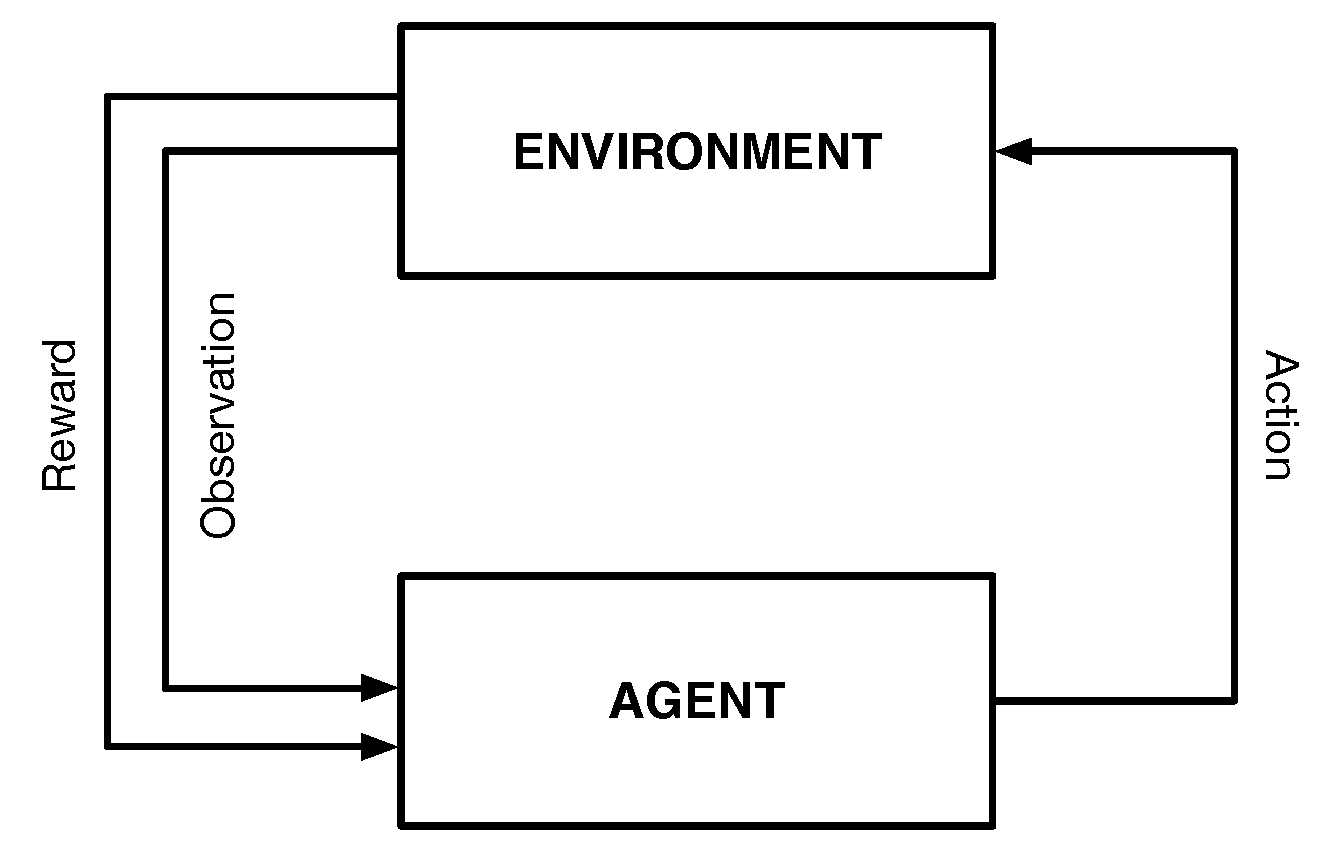
\includegraphics[width=\textwidth]{images/agent-environment.pdf}
\caption{The reinforcement learning process}
\label{fig:agentandenvironment}
\end{figure}

The reinforcement learning problem is modeled as a sequential decision problem, see figure \ref{fig:agentandenvironment} for a graphical representation of the process. A learning algorithm, an agent, performs an action and receives a reward according to some measure of how desirable the results of the action are.  After the action is taken, the state of the environment changes and the agent then receives a new observation of it, and then the process repeats. The goal of the reinforcement learning agent is to maximize the reward received over a certain time period, finding a balance between immediate and future rewards \parencite{barto1998reinforcement}. 


%One thing that sets reinforcement learning apart from other fields within artificial intelligence is that a reinforcement learning problem is solved by an online algorithm. That is, a reinforcement learning algorithm learns about its task and environment while operating in the environment. The actions taken by the agent affect what it knows about the environment, and thus its appraisal of the value of future actions and/or states of the environment.


There are several ways of further dividing reinforcement learning problems into other subcategories. Some examples are the dichotomies 1) episodic/non-episodic problems 2) problems with continuous/discrete state spaces 3) problems with continuous/discrete action spaces 4) problems with one/multiple concurrent agents. (etc.) In the text below, the two first of these dichotomies, which are relevant to this thesis, are discussed. 

\subsection{Episodic and Non-episodic Problems}
One can categorize reinforcement learning problems based on whether or not the time steps are divided into episodes. When the time steps for the agent-environment interaction are divided into subsequences in this manner, the problem is called episodic. This is common in for example games, which end when they are won or lost. If the problem is not episodic, it is called non-episodic, which means, consequently, that the interaction is not divided into subsequences. Instead, the interaction between the actor and environment goes on continually without end \parencite{barto1998reinforcement}. Two examples of non-episodic applications are controlling a robot arm (as well as other robotics problems) and maneuvering a helicopter \parencite{ng2006autonomous}. 

\subsection{Continuous and Discrete Problems}
An alternative way to categorize reinforcement learning problems is based on whether their state spaces are continuous or discrete. An important difference between the two kinds of problems is how an agent can treat similar states in the model. In a continuous problem it is a lot easier to group together states located around the same ``position'' due to the nature of a continuous problem, where the states usually more or less meld together. For example, if the reinforcement learning problem is to control a robot arm whose position is the state of the environment, the different states located around the same general area are not very different. This means that they might be treated in the same way or a similar way by an agent. On the other hand, consider the discrete problem of a game of connect four, wherein the placement of a coin into one of two adjacent slots could dramatically change the evaluation of the state and the outcome of the game \parencite{barto1998reinforcement}.

psection{Markov decision process}

Within reinforcement learning, the concept of Markov secision processes (MDP) is central. An MDP is a way to model an environment where state changes in it are dependent on both random chance and the actions of an agent. An MDP is defined by the quadruple $\left( S, A, P( \cdot , \cdot, \cdot ) , R( \cdot , \cdot ) \right)$ \parencite{altman2002applications}: 

\begin{description}
\item[$S$] \hfill \\ 
    A set of states representing the environment.
\item[$A$] \hfill \\ 
    A set of actions that can be taken.
\item[$P \colon S \times A \times S \to \mathbb R$] \hfill \\ 
    A probability distribution over the transitions in the environment. This function describes the probability of ending up in a certain target state when a certain action is taken from a certain origin state. 
\item[$R \colon S \times A \to \mathbb{R}$] \hfill \\ 
    A function for the reward associated with a state transition. In some formulation of MDPs the reward function only depends on the state.
\end{description}

MDPs are similar to Markov chains, but there are two differences. First, there is a concept of rewards in MDPs, which is absent in Markov chains. Second, in a Markov chain, the only thing that affects the probabilities of transitioning to other states is the current state, whereas in an MPD both the current state and the action taken in that state are needed to know the probability distribution connected with the next state \parencite{altman2002applications}.


\input{Technical_Background/MDP/markov_property.tex}
\input{Technical_Background/MDP/sparse_mdps.tex}
\input{Technical_Background/MDP/factored_representations.tex}


\section{Basic algorithms for solving MDPs}

A policy $\pi$ is a function from a state $s$ to an action $a$ that operates in
the context of a Markov Decision Process, i.e. $\pi \colon S \to A$. A policy
is thus a description of how to act in each state of an MDP. An arbitrary
policy is denoted by $\pi$ and the optimal policy (the policy with the largest
expected reward in the MDP) is denoted by $*$. The rest of this section is
describes some basic algorithms for solving, that is to say finding an optimal
policy, in an MDP.

\subsection{Value functions}

To solve an MDP most algorithms uses an estimation of values of states or
actions. Two value functions are usually defined, the state-value function $V :
S \to \mathbb R$ and the state-action-value function $Q : S \times A \to
\mathbb R$. As the names implies $V$ signifies how good a state is, while $Q$
signifies how good an action in a state is. The state-value function,
$V^\pi(s)$, returns the expected value when starting in state $s$ and following
policy $\pi$ thereafter. Equations \eqref{equation:v_finite} and \eqref{equation:v_infinite} show the equations for the state-value function for a finite time horizon and an infinite, discounted, time horizon respectively. In \eqref{equation:v_infinite}, $\gamma$ is the discount factor, a value between 0 and 1 which describes how fast the value of expected future rewards decay as one looks further into the future. The state-action-value function $Q^\pi(s, a)$ returns
the expected value when starting in state $s$ and taking action $a$ and
thereafter following policy $\pi$. The value functions for the optimal policy
are denoted by $V^*(s)$ and $Q^*(s, a)$. Formulas for the state-action value functions are anologous to those presented for the state value functions. 

\begin{align}
\label{equation:v_finite}
V_t^\pi(s) = \mathbb{E} \{ \sum_{k=0}^{T=k} r_{t+k} | S_t = S, \pi \}
\end{align}

\begin{align}
\label{equation:v_infinite}
V_{0}^\pi(s) = \mathbb{E} \{ \sum_{t=0}^\infty r_{t}\gamma^t | S_0 = S,\pi \}
\end{align}

Both $V^\pi$ and $Q^\pi$ can be estimated from experience. This can be done by
maintaining the average of the rewards that have followed each state when
following the policy $\pi$. When the number of times the state has been
encountered goes to infinity, the average over these histories of rewards
converges to the true values of the value function
\parencite{barto1998reinforcement}.

\input{Technical_Background/ValueFunctions/dynamic_programming.tex}
\input{Technical_Background/ValueFunctions/policy_iteration.tex}
\input{Technical_Background/ValueFunctions/value_iteration.tex}


\subsection{\etre\ in Factored Markov Decision Processes 
\note{N}}
\label{sec:e3_factored_discussion}

\paragraph{General shape of the results} In a comparison of the \etre\ agent's behavior in the different-size environments, the similarity of the shape of the graphs is striking. At first there is a period of lower and lower performance. (For the smallest environments, this period is very short, however.) Next, there is a period of fairly constant high performance, which lasts until the end of the experiment.  

This shape can be explained as a consequence of the different phases of operation of the \etre\ algorithm coupled with the structure of the MDP studied. In the beginning of the experiment, the algorithm will spend almost all of its time in the balanced wandering and exploration phases. The longer the agent has been exploring, and the more states become known, the further the agent has to explore into hard-to-reach parts of the MDP to find unexplored states. Now, in the case of the invasive species environment with the parameters chosen as in the experiments presented, the most easily reachable states are the ones where there is no tamarisk infection. This means that the harder a state is to reach, the more infected it will be, and thus the performance of the \etre\ agent in the exploration phase will fall as the experiment progresses. 

However, once the agent knows enough about the environment to enter the exploitation phase, the \etre\ agent spends close to no time at all exploring unknown states, and it retains high performance. 

\paragraph{Consequences of pooling observation data} An interesting result is that the agent is able to enter the exploitation phase for the 10 reaches/1 habitat per reach test setup slightly earlier than for the 5 reaches/1 habitat per reach setup. This is probably connected to the optimization described in the last paragraph of section \ref{sec:factored_e3}. In the 10 reaches/1 habitat per reach case there are nine reaches with two parents (including the reach itself) and one reach with only itself as parent. In the 5 reaches/1 habitat per reach case there are four reaches with two parents and one reach with only itself as parent. Since observations for state variables with similar parent structure are pooled by our \etre\ implementation, the agent will receive almost double the information per time step for the two-parent reaches in the 10 reaches case as compared to the 5 reaches case.  

\paragraph{Possible issues with the one-policy-per-reach optimization} In section \ref{sec:one_policy_per_state_variable} an optimization is described that works very well for the particular environment and environment settings that the agent was tested for. However, this optimization makes several assumptions that may cause problems if the settings are changed. For instance, one assumption is that the state of a reach is only affected directly by its adjacent parents in the DBN. If the state of a reach was made to depend significantly on other reaches two or more levels up in the river network, the agent would probably not be able to converge on an optimal policy. 

Another assumption that could lead to problems with other environment settings is the assumption that the maximal action cost in the environment is impossible or very hard to break. The invasive species environment has a maximum cost for actions. However, with the standard settings it is mathematically impossible to break this maximum. Our implementation of \etre\ would achieve very poor performance if this was not the case, since a large penalty is given when the maximum action cost is breached. 

\paragraph{DBN structure} Finally, in the invasive species environment, the structure of the DBN underlying the MDP is known at the start of the experiment, so the agent does not need to infer it from its observations. If this was not the case, all the DBN optimizations would be useless unless some kind of algorithm for infering the DBN structure was added to the agent. 

\chapter{Environment and algorithms}
\label{ch:algo}

This chapter gives a description of the environment and the algorithms that
were used in the experiment described in chapter \ref{ch:method}. The environment Invasive Species, is a simulation of a river network with invading species where to goal is to eradicate unwanted species and is further described in section \ref{sec:experiment_env}. 

Two algorithms are covered in this chapter, both of which deal with the
problems that arise with large state spaces; however, they differ in the
methods they apply. In the following chapter the general ideas behind the
algorithms, as well as specific details, are presented. 

The model-based interval estimation algorithm, described in
section~\ref{sec:mbie}, utilizes clever estimations of confidence intervals for
the Q-value functions to improve performance in sparse MDPs.
Section~\ref{sec:fac_e3} is on an algorithm that uses dynamic bayesian networks
and factored representations to improve the \etre\ algorithm to efficiently
deal with factored MDPs. 

\section{Environment specification, Invasive Species}
\label{sec:experiment_env}

When the agents were tested, the Invasive Species environment from the 2014 edition of
the Reinforcement Learning Competition was used. The environment is a
simulation of an invasive species problem, in this case a river network with
invading species where the goal of the agent is to eradicate unwanted species
while replanting native species. 

The environment's model of the river network has parameters, such as the size
of the river network and the rate at which plants spread, which can be
configured in order to create different variations of the environment.  The
size of the river network is defined by two parameters: the number of reaches
and the number of habitats per reach. A habitat is the smallest unit of land
that is considered in the problem. A habitat can either be invaded by the
tamarix, which is an unwanted species, empty or occupied by native species. A
reach is a collection of neighboring habitats. The structure of the river
network is defined in terms of which reach is connected to which
\parencite{invasiveSpecis2014:Online}. In figure \ref{fig:river} a model of a
river network is shown.

\begin{figure}[ht]
\centering
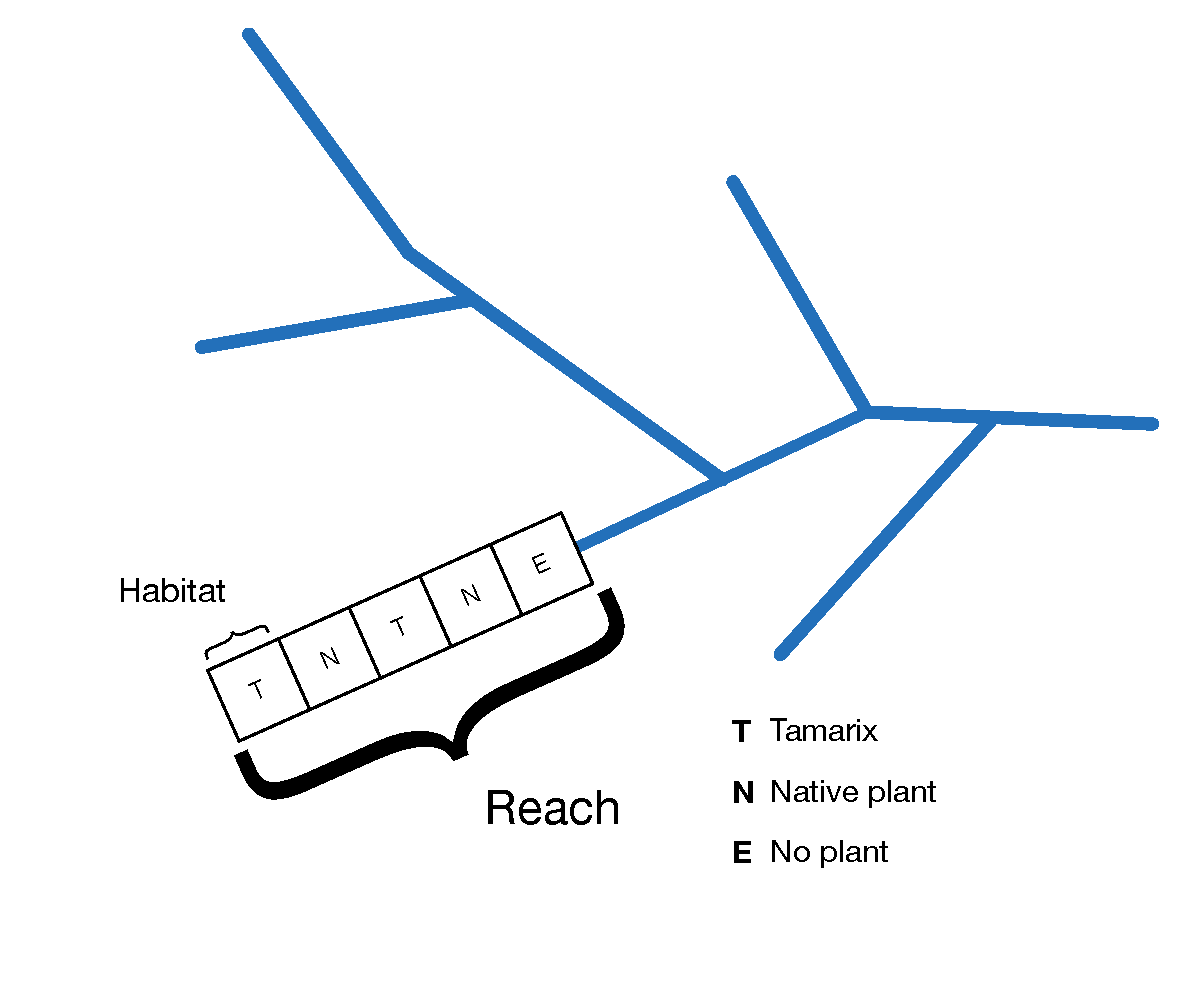
\includegraphics[width=0.9\textwidth]{images/river_network.pdf}
\caption{A river network, as modeled by the Invasive Species reinforcement learning environment.}
\label{fig:river}
\end{figure}

There are four possible actions (eradicate tamarix trees, plant native trees,
eradicate tamarix trees and plant native trees and a wait-and-see action),
and the agent chooses one of these actions for each reach and time step. If the 
agent chooses to eradicate tamarix trees or plant native trees in a reach, 
all habitats of that reach are targeted by this action. What
actions are available to the agent depends on the state of each reach. It is
always possible to choose the wait-and-see action, but there has to be one
or more tamarix-invaded habitats in a reach for the eradicate or eradicate and
plant actions to be available and there has to be at least one empty habitat in
a reach for the plant-native-trees action to be available
\parencite{invasiveSpecis2014:Online}.  

\section{Model-based interval estimation}
\label{sec:mbie}

Model-based interval estimation is a modification of value iteration whose main feature is its  addition of confidence
intervals to the state-action values. These confidence intervals allow the agent to choose between
actions, based on how confident it is about its evaluation of them. In effect,
the less certain the agent is about its evaluation of the states and actions,
the more exploratory the actions will be. When the agent is more confident
however, it will exploit what it has learnt so far about the MDP
\parencite{dietterich2013pac}.

\input{algorithms/MBIE/modification_of_value_it}
\input{algorithms/MBIE/gt.tex}
\input{algorithms/MBIE/modded_bounds}

\section{\etre\ in factored Markov decision processes}
\label{sec:fac_e3}

The second algorithm studied in this thesis is a version of the \etre\ algorithm that focuses on factored problem domains by modeling them as a dynamic Bayesian network. The original \etre\ algorithm is described in section \ref{sec:e3}, which gives a broad overview along with the key strategies used in the algorithm. The following section, \ref{sec:factored_e3}, considers some ways to extend the original algorithm and make use of factored representations and planning in factored domains to improve the running time of the algorithm.

\input{algorithms/Factored_E3/e3.tex}
\input{algorithms/Factored_E3/factored_additions.tex}


\chapter{Method}
\label{sec:method_intro}

This chapter covers the preliminaries and preparations carried out before the
execution of the experiments. It covers  and how the agents described in chapter
\ref{ch:algo} were implemented and the additions and modifications that were made to them. The chapter
concludes with a description of the tools used for the experiment.
\section{Algorithm implementation}
\label{sec:implementation}

We implemented two existing algorithms and we also added some extensions.  The
experiment utilized RL-Glue (section~\ref{sec:rl_glue}) to connect the agents
and environment to each other.  To verify the behavior of our agents we utilized smaller
environments (see sections~\ref{sec:intro_grid_world} and \ref{sec:ns}) where
the correct operation is either easy to derive or obvious from inspection. By
starting with smaller problems and using an iterative approach it was possible
to identify bottlenecks in our implementations and correct possible errors
early.

\input{algorithms/MBIE/modded_bounds}

\input{method/ConstructingExperiments/contributionse3}

\subsection{GridWorld}
\label{sec:intro_grid_world}

The GridWorld environment was implemented to easily be able to verify the
correctness of the MBIE algorithm. It consists of a grid of twelve squares with
one blocked square, one starting square, one winning square, one losing square and
eight empty squares. The agent can take five actions, north, south, west,
east or exit. The exit-action is only possible from the winning or losing
state. When taking an action being in one state and the action is directed to
another empty state there is an 80\% probability to succeed and 10\%
probability to fail and 10\% to go sideways.

\subsection{Network simulator}
\label{sec:ns}

A simple computer network simulation was implemented to verify the behavior of an
early version of \etre\ algorithm. In this environment, the agent tries to keep
a network of computers up and running. All computers start in the running
state, but there is a chance that they randomly stop working. If a computer is
down, it has a chance to cause other computers connected to it to also fail. In
each time step, the agent chooses one computer to restart, which with 100
percent probability will be in working condition in the next time step. The
agent is rewarded for each computer in the running state after each time step. 

\section{Our contributions}
\label{sec:contributions}


\input{algorithms/MBIE/modded_bounds}


\input{method/ConstructingExperiments/contributionse3}

\section{Environment specification}
\label{sec:experiment_env}

For the experiment, the Invasive Species environment from the 2014 edition of
the Reinforcement Learning Competition was used. The environment is a
simulation of an invasive species problem, in this case a river network with
invading species where the goal of the agent is to eradicate unwanted species
while replanting native species. 

The environment's model of the river network has parameters, such as the size
of the river network and the rate at which plants spread, which can be
configured in order to create different variations of the environment.  The
size of the river network is defined by two parameters: the number of reaches
and the number of habitats per reach. A habitat is the smallest unit of land
that is considered in the problem. A habitat can either be invaded by the
tamarix, which is an unwanted species, empty or occupied by native species. A
reach is a collection of neighboring habitats. The structure of the river
network is defined in terms of which reach is connected to which
\parencite{invasiveSpecis2014:Online}. In figure \ref{fig:river} a model of a
river network is shown.

\begin{figure}[ht]
\centering
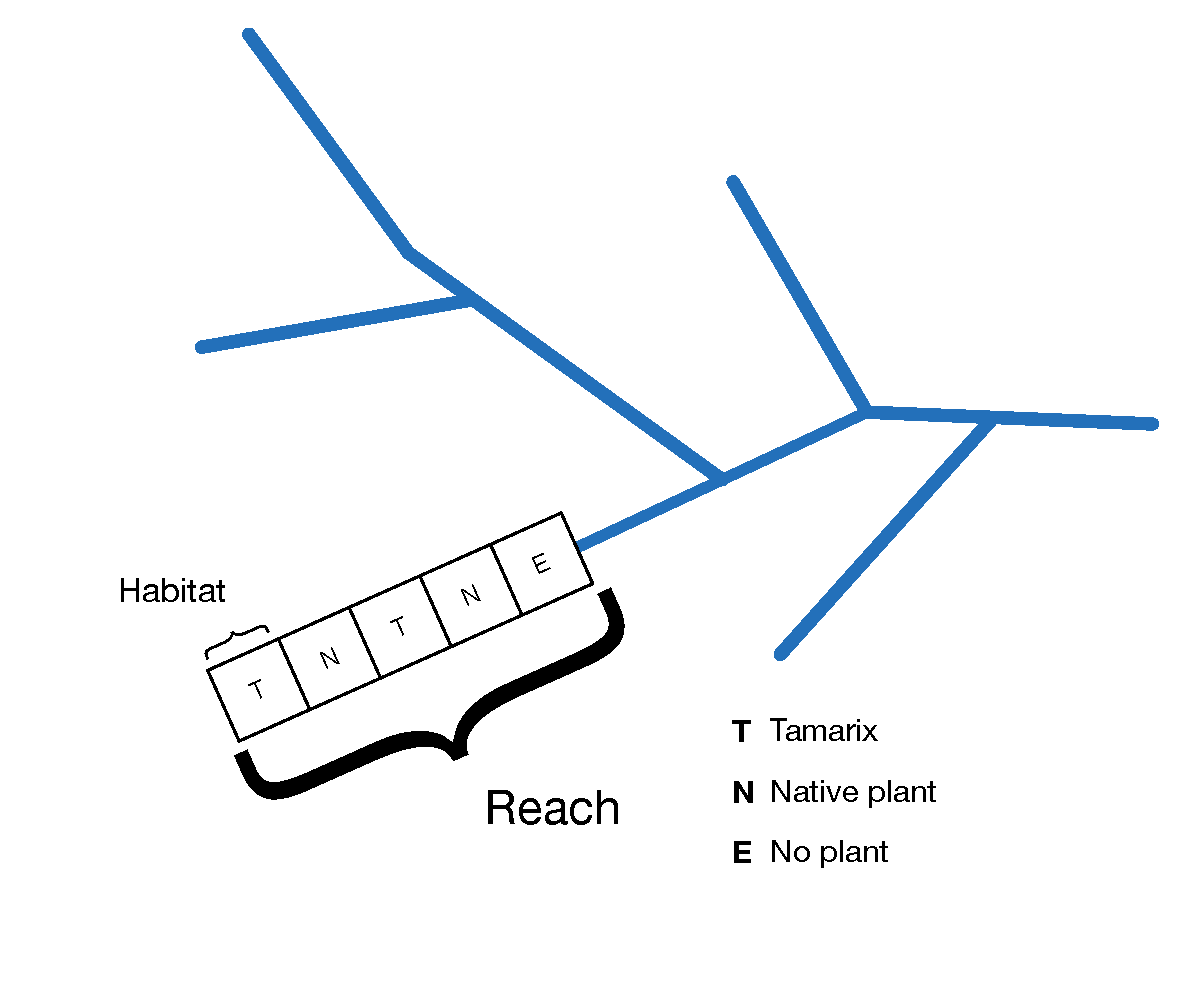
\includegraphics[width=0.9\textwidth]{images/river_network.pdf}
\caption{A river network, as modelled by the Invasive Species reinforcement learning environment.}
\label{fig:river}
\end{figure}

There are four possible actions (eradicate tamarisks, plant native trees,
eradicate tamarisks and plant native trees, and finally a wait-and-see action),
and the agent chooses one of these actions per reach per time step. What
actions are available to the agent depends on the state of each reach. It is
always possible to choose the wait-and-see action, but there has to be one
or more tamarix-invaded habitats in a reach for the eradicate or eradicate and
plant actions to be available and there has to be at least one empty habitat in
a reach for the plant-native-trees action to be avalable
\parencite{invasiveSpecis2014:Online}. 

\section{Test specification}
\label{sec:test_spec}

The testing of the agents required us to choose certain sets of parameters, for
the environment, the two different agents and the experiment itself. 

\paragraph{Environment parameters}

The Invasive Species environment requires a number of parameters. For further
explanation of the environment parameters consult the environment
webpage\footnote{\url{http://2013.rl-competition.org/domains/invasive-species}}.
The specific parameters used are presented in
appendix~\ref{ap:environment_spec}.

\paragraph{Agent Parameters}

The agents evaluated required different types of parameters. Some preliminary
tests were run and then the parameters giving best results were chosen.
Parameters for MBIE are found in table~\ref{tab:mbie_params_both}.

\begin{table}[H]
\centering
\captionof{table}{Parameters for MBIE}
\label{tab:mbie_params_both}

\begin{subfigure}[b]{0.47\textwidth}
    \centering
    \captionof{table}{Proper MBIE}
    \label{tab:mbie_params} 
    \begin{tabular}{lr}
     \toprule
     Parameter & Value \\
     \midrule
     Discount factor, $\gamma$ & 0.9 \\
     Confidence, $\delta$ & 95\% \\
     $\Delta \omega$ & $\frac{1}{2}\sqrt{\frac{2|ln(2^{|S|}-2) - ln  \delta |}{N(s,a)}}$ \\
     
     \bottomrule
    \end{tabular}
\end{subfigure}
\quad
\begin{subfigure}[b]{0.47\textwidth}
    \centering
    \captionof{table}{Realistic MBIE}
    \label{tab:mbie_realistic_params}
    \begin{tabular}{lr}
     \toprule
     Parameter & Value \\
     \midrule
     Discount factor, $\gamma$ & 0.9 \\
     $\Delta \omega$ & $1 - 0.05 N(s,a)$ \\
     \bottomrule
    \end{tabular}
\end{subfigure}
\end{table}

For DBN-\etre\ a higher exploration limit resulted in the agent starting to
exploit earlier but with a slightly lower final return. A higher partial state
known limit resulted in later exploitation but no appreciable difference in
final return. The values in table~\ref{tab:dbne3_params} were a good middle
ground.

\begin{table}[H]
\captionof{table}{DBN-\etre\ parameters}
\label{tab:dbne3_params}
\centering
\begin{tabular}{lr}
 \toprule
 Parameter & Value \\
 \midrule
 Discount factor & 0.9 \\
 Exploration limit & 5\% \\
 Partial state known limit & 5 \\
 \bottomrule
\end{tabular}
\end{table}

\paragraph{Experiment parameters}

The tests performed had to be long enough to sample enough data to extract
relevant results without making the running time too long. A single test
consisted of a specific number of episodes with a specific length. A good
combination was required to efficiently evaluate the agents. If a single
episode consisted of too many samples it would be difficult to see the learning
process as results are reported as total reward over an episode and that
process might be hidden as its impact on the total reward is smaller with a
longer episode. On the other hand, if an episode length is too short it would
end before the agents could do any valuable learning.

In addition to a satisfactory episode length, a reasonable number of episodes
needs to be sampled for it to be possible to draw conclusions from the results.
If the number of episodes is too small, the convergence of the agents cannot be
seen. However, if the number of episodes are too large a lot of sampled data
would be redundant for the study. Some preliminary experiments were run in
order to tune the experiment parameters to suitable values. The episode length
was set to 100 samples and there were 100 episodes per test.

To evaluate the agents in the Invasive Species environment combinations of
reaches and number of habitats per reach that can be seen in
table~\ref{tab:reaches_habitats} were choosen. Combinations were chosen to have
a wide range in the total number of states for the agents to deal with and to
test how the agents deal with taking actions that have to take into account
several state components. 

As seen in table ~\ref{tab:reaches_habitats}, the state count increases rapidly
when habitats are added to the problem. This is obvious from the fact that the state count
depends exponentially on the total number of habitats; see equation \eqref{eq:statecount}, where $h$ is the number of habitats per reach and $r$ is the number of reaches.

\begin{equation}
\label{eq:statecount}
 |S| = 3 ^ {hr}
\end{equation}

\begin{table}[H]
\centering
\caption{Combinations of reaches and habitats used in testing.}
\label{tab:reaches_habitats}
\begin{tabular}{rrr}
 \toprule
 Reaches & Habitats per reach & Total state count \\
 \midrule
 5  & 1 &          243 \\
 3  & 2 &          729 \\
 3  & 3 &      19\,683 \\
 10 & 1 &      59\,049 \\
 4  & 3 &     531\,441 \\
 5  & 3 & 14\,348\,907 \\
 \bottomrule
\end{tabular}
\end{table}

\section{Programming environment}
\label{sec:prog_env}

The Java programming language 1.7 was used to implement the algorithms. In addition, the
Java version of RL-Glue framework version 3.0 was used. For version control Git
was used, due to its simplicity and performance.

\section{RL-Glue}
\label{sec:rl_glue}

To evaluate the agents the RL-Glue framework was used, which acts as an
interface for communication between the agent and the environment. The software
uses the RL-Glue protocol, which specifies how a reinforcement learning problem
should be divided when constructing experiments and how the different programs
should communicate \parencite{tanner2009rl}.

RL-Glue divides the reinforcement learning process into three separate
programs: an agent, an environment and an experiment. RL-Glue provides a server
software that manages the communication between these programs. The agent and
the environment programs are responsible for executing the tasks as specified
by RL-Glue and the experiment program acts as a bridge between the agent and
environment \parencite{tanner2009rl}.

The modular structure of RL-Glue makes it easier to construct repeatable
reinforcement learning experiments. By separating the agent from the
environment it is possible to reuse the environment and switch out the agent.
It also makes it a lot easier to cooperate and continue working on existing
environments implemented by other programmers.


\chapter{Result}

\newcommand{\graphwidth}{0.70\textwidth}
\newcommand{\testsubfigure}[2]{%
\begin{subfigure}[b]{\graphwidth}
    \includegraphics[width=1.1\textwidth]{images/tests/#1r-#2h.pdf}
    \caption{#1 reaches and #2 habitats per reach}
    \label{fig:#1r#2h}
\end{subfigure}
}

In figures~\ref{fig:tests1}, \ref{fig:tests2} and \ref{fig:tests3} we have test results from running our agents on the invasive species environment on different sizes of river network. The raw data can be found in appendix~\ref{ap:result_tables}.

\begin{figure}[h!]
    \centerline{
    \testsubfigure{3}{3}
    ~
    \testsubfigure{3}{2}
    }
    \caption{Test runs with different number of reaches and habitats}
    \label{fig:tests1}
\end{figure}

\begin{figure}[h!]
    \centerline{
    \testsubfigure{5}{1}
    ~
    \testsubfigure{5}{3}
    }
    \caption{Test runs with different number of reaches and habitats}
    \label{fig:tests2}
\end{figure}

\begin{figure}[h!]
    \centerline{
    \testsubfigure{4}{3}
    ~
    \testsubfigure{10}{1}
    }
    \caption{Test runs with different number of reaches and habitats}
    \label{fig:tests3}
\end{figure}

The agent learns for 100 episodes with 100 samples per episode, other parameters are specified in section~\ref{sec:test_spec}. The invasive species environment associates a certain cost with each state and action, thus the reward is always negative. In each test the reward varies over time for the MBIE agent, the realistic MBIE agent and the DBN-\etre\ agent.

With smaller state spaces (see figure~\ref{fig:3r3h}, \ref{fig:3r2h} and \ref{fig:5r1h}) we can see that the realistic MBIE agent outperforms the proper MBIE agent and comes close to the DBN-\etre\ agent. In the tests where the state space is larger (see figure~\ref{fig:5r3h}, \ref{fig:10r1h} and \ref{fig:4r3h}) proper MBIE and realistic MBIE are very close to each other in performance while the DBN-\etre\ agent outperforms both. The realistic MBIE algorithm performs better in with smaller state spaces due to more states becoming known quicker and thus having their true value.

In each of the test runs the DBN-\etre\ algorithm exhibits a period of learning that corresponds to exploration (as described in section~\ref{sec:e3}) where the agent has not explored the environment enough and seeks more information. This is apparent in figure~\ref{fig:3r3h}.
\chapter{Discussion \note{B}}
\label{ch:discussion}
This chapter is a discussion of the results and method used in the project. The algorithms are evaluated with regard to their performance achieved in the tests, which is used as a basis when comparing them against each-other. Determining their strengths and weaknesses and if they were suitable for problems with an environment that has a large discrete state space and in particular for the environment Invasive Species. There is also a discussion on ethical aspects regarding the work in this thesis.


% Det behövs inte en ingående disposition här, det tar ner läsligheten. Det som tas upp i styckena är vettigt, men detta är inte rätt ställe för dem.

% This chapter is a combination of discussion of the results of using the algorithms described in chapter \ref{ch:algo}, together with a examination of the method used in the project. The algorithms is evaluated with regard to their performance achieved in the experiments \ref{sec:constructing_experiments}, which is used for a basis when comparing them against each-other. Focusing on their strengths and weaknesses and circling around the question why did they perform as they did. Were they suitable for this kind of problem, an environment with a large discrete state space and in particular for this thesis a simulation of an Invasive Species environment.

% The second part of this chapter contains a section containing a presentation of similar studies conducted, summarizing their results and opinions. Using their finding as a basis, there will also be a discussion regarding its connection to the results in this thesis. With inspiration from similar studies in combination with the results of this thesis, a discussion about the possible extensions and additional work or unanswered questions in this thesis are presented. 

%In order to round of this chapter, the last section of this chapter revolves around ethical questions and aspects regarding the theme of this topic. The main theme of the last section is ethical aspects in \acrlong{ai} \acrshort{ai}, \acrfull{ai}, along with a discussion about the usefulness of Reinforcement Learning in today's society with focus on using simulations.

\section{Evaluation of the agents \note{I}}
\label{sec:coa}

\input{Discussion/AlgorithmsEvaluation/dbn.tex}
\input{Discussion/AlgorithmsEvaluation/mbie.tex}
\input{Discussion/AlgorithmsEvaluation/discussion_diffrences}




\section{Potential factors impacting the results}
\label{sec:truth_results}

There are several factors that possibly reduce the reliability of the results. For instance, all evaluations used only one environment, the implementation of the algorithms could contain errors and the correct results for all test runs are not always known. 

\input{Discussion/discussion_results/impact_of_one_env.tex}

\input{Discussion/discussion_results/implementation_of_algorithms.tex}

\input{Discussion/discussion_results/testing_methodology.tex}


%\section{Similar Studies \note{N, K}}
The work with reducing the complexity of the reinforcement learning problems with environments containing large state spaces is not a new research topic. However, this thesis is taking a rather uncommon approach to the problem. Instead of trying to derive new algorithms for solving the problem, the focus is instead focused on usefulness of research conducted within the area of reinforcement learning problems. To be even more specific this thesis has zoomed in on two possible attempts on solving the problem with environments containing large state spaces. An approach that is rather uncommon and thus similar studies is as well uncommon. 
%Behöver skrivas om, tydligare
Thereby this section will combining focus on both studies similar to this thesis comparing the usefulness of research already conducted along with a summarized study of studies of work being done to reduce the complexity of environments with large state spaces.

\todo[inline]{Samma miljö kanske, dess pac?}

\paragraph{Similar Studies Regarding Comparing Existing Research}
\todo[inline]{Borde finnas återkoppling i diskussion kring detta}
It has been shown in Strehl and Littman (2004; 2008) that MBIE outperforms \etre\ in the MDPs RiverSwim and SixArms. \parencite{dietterich2013pac}


\paragraph{Large State Spaces using Dynamic Bayesian Networks}
This paragraph is devoted to similar methods using dynamic Bayesian networks as an underlying representation in order to model the structure of the environment. Due to the relevance of using dynamic Bayesian network as a method for tackling similar problems it is thesis on its own in order to summarize them all. It is also possible to study section \ref{sec:better_planing_algos} for further references, however their main focus on the planning algorithm.

An algorithm to DBN-\etre\ is the algorithm by \textcite{ross2012model} which is as well utilizing a factored representation for the underlying structure. However, in the DBN-\etre\ algorithm no planning algorithm was specified and therefore leaving an empty square in the implementation affecting the overall complexity of the algorithm. In the algorithm by \textcite{ross2012model} 

\todo[inline]{Resultatjämförelse}

\paragraph{Similar Studies Regarding Large State Spaces Using Model Based Something grejen}
Grattis MBIE, er punkt.

\section{Ethical and social aspects of artificial intelligence}

\input{Discussion/Ethics/intro.tex}

\input{Discussion/Ethics/invasive_species.tex}

\input{Discussion/Ethics/ai_right_or_wrong.tex}



\section{Further work}

In this section we discuss possible further work and extensions to our thesis.

\input{Discussion/further_work/more_test_envs.tex}
\input{Discussion/further_work/better_planning_dbn.tex}
\input{Discussion/further_work/MBIE.tex}
\input{Discussion/further_work/mbie_should_use_dbn.tex}


\printbibliography

\begin{appendices}

\chapter{Environment specification}
\label{sec:environment_spec}

\begin{table}[H]
\centering
\captionof{table}{Dynamic parameters common to both species}
\label{tab:dynamic_params_common} 
\begin{tabular}{l r}
 \toprule
 Parameter & Value \\
 \midrule
 Eradication rate & 0.85 \\
 Restoration rate & 0.65 \\
 Downstream spread rate & 0.5 \\
 Upstream spread rate & 0.1 \\
 \bottomrule
\end{tabular}
\end{table}

\begin{table}[H]
\centering
\captionof{table}{Dynamic parameters different between the species} \label{tab:dynamic_params_not_common}
\begin{tabular}{lrr}
\toprule
 Parameter & Native & Tamarisk \\
 \midrule
 Death rate & 0.2 & 0.2 \\
 Production rate & 200 & 200 \\
 Exogenous arrival\footnote{Arrival of seeds from outside the environment} & Yes & Yes \\
 Exogenous arrival probability & 0.1 & 0.1 \\
 Exogenous arrival number & 150 & 150 \\
 \bottomrule
\end{tabular}
\end{table}

\begin{table}[H]
\centering
\captionof{table}{Cost function parameters} \label{tab:cost_params} 
\begin{tabular}{lr}
 \toprule
 Parameter & Value \\
 \midrule
 Cost per invaded reach & 10 \\
 Cost per tree & 0.1 \\
 Cost per empty slot & 0.01 \\
 Eradication cost & 0.5 \\
 Restoration cost & 0.9 \\
 \bottomrule
\end{tabular}
\end{table}

\begin{table}[H]
\centering
 \captionof{table}{Variable costs depending on number of habitats affected by action}
 \begin{tabular}{lr}
 \toprule
 Parameter & Value \\
 \midrule
 Eradication cost & 0.4 \\
 Restoration cost for empty slot & 0.4 \\
 Restoration cost for invaded slot & 0.8 \\
 \bottomrule
\end{tabular}
\label{tab:cost_params_var}
\end{table}
\end{appendices}


\end{document}

\RequirePackage[l2tabu,orthodox]{nag}

\documentclass[bachelors,a4paper]{chalmers-thesis}

\usepackage[swedish, english]{babel}

\usepackage[utf8]{inputenc}
\usepackage{comment}
\usepackage{color}
\usepackage{todonotes}
\usepackage{hyperref}


% To be able to include pdfs in the document
\usepackage{pdfpages}

% To use appendices
\usepackage[toc,page]{appendix}

% Fancy maths!
\usepackage{amsmath}
\usepackage{amssymb}

% Fancy references
\usepackage[style=authoryear,date=iso8601]{biblatex}
\addbibresource{jelzin.bib}

% Fancy graphics
\usepackage{graphicx}

% For the finest tables
\usepackage{booktabs}
\usepackage{longtable}

% For mutliple column pages
\usepackage{multicol}

% For the finest of subfigures in figures or tables
\usepackage{subcaption}

% To be able to position figure envs exactly where you want them use H.
\usepackage{float}

% Nice environments for pseudocode
\usepackage[chapter]{algorithm}
\usepackage{algpseudocode}

\title{Reinforcement learning}
\subtitle{A comparison of learning agents in environments with large discrete state spaces}
\author{%
Johan Andersson\and
Emil Kristiansson\and
Joakim Persson\and
Adam Sandberg Eriksson\and
Daniel Toom\and
Joppe Widstam}
\thesisin{Computer Science}
\department{Department of Computer Science and Engineering}
\reportno{2014:05}
\copyrightyear{2014}
\keywords{Reinforcement learning, Artificial intelligence, MBIE, DBN-\etre, Invasive Species, Learning algorithms}

% Abstracts
\firstabstract{% 1 Motivation

For some real-world behavior optimization problems, it is infeasible to search for a solution by making a model of the problem and performing calculations on it. 
In cases like these, good solutions can sometimes be found by trial and error. 
Reinforcement learning is a way of finding optimal behavior by systematic trial and error.
% 2 Problem statement
This thesis aims to compare different reinforcement learning techniques and evaluate them. 
Model-based interval estimation (MBIE) and Explicit explore or exploit using dynamic bayesian networks - (DBN-\etre)
 are two algorithms that are evaluated. 
% 3 Approach
To evaluate the techniques, learning agents were constructed using the algorithms and 
then simulated in the environment invasive species from the reinforcement learning competition.
% 4 Results
The results of the study show that an optimized version of DBN-\etre\ is better than MBIE at finding an optimal or near optimal behavior policy in the 
environment invasive species for a selection of environment parameters.

% 5 Conclusions
Using a factored model like a DBN shows certain advantages operating in 
the factored environment invasive species. For example it achieves a near optimal
policy within fewer episodes than MBIE.


% Följande saker ska vara med i en abstract Motivation, Problem Statement, Approach, REsults

% Motivation
% Why do we care about the problem and the results? 
% If the problem isn't obviously "interesting" it might be better to
% put motivation first; but if your work is incremental progress on
% a problem that is widely recognized as important, then it is 
% probably better to put the problem statement first to indicate which
%  piece of the larger problem you are breaking off to work on.
% This section should include the importance of your work, the difficulty
% of the area, and the impact it might have if successful.

% Problem statement
% What problem are you trying to solve? What is the scope of your work 
%(a generalized approach, or for a specific situation)? Be careful not to 
% use too much jargon. In some cases it is appropriate to put the problem 
% statement before the motivation, but usually this only works if most 
% readers already understand why the problem is important.

% Approach
% How did you go about solving or making progress on the problem? Did you 
% use simulation, analytic models, prototype construction, or analysis of
% field data for an actual product? What was the extent of your work
% (did you look at one application program or a hundred programs in
% twenty different programming languages?) What important variables did
% you control, ignore, or measure?

% Results
% What's the answer? Specifically, most good computer architecture papers 
% conclude that something is so many percent faster, cheaper, smaller, 
% or otherwise better than something else. Put the result there, in
% numbers. Avoid vague, hand-waving results such as "very", "small",
% or "significant." If you must be vague, you are only given license
% to do so when you can talk about orders-of-magnitude improvement. 
% There is a tension here in that you should not provide numbers that
% can be easily misinterpreted, but on the other hand you don't have
% room for all the caveats.

% Conclusions
% What are the implications of your answer? Is it going to change the 
% world (unlikely), be a significant "win", be a nice hack, or simply 
% serve as a road sign indicating that this path is a waste of time 
% (all of the previous results are useful). Are your results general, 
% potentially generalizable, or specific to a particular case?
}
\secondabstract{swedish}{% 1 Motivation
För vissa verklighetsbaserade optimeringsproblem där det gäller att finna ett bästa beteende är det orimligt söka efter det optimala beteendet genom att skapa en modell av problemet och sedan utföra beräkningar på den. I vissa sådana fall kan man hitta bra lösningar genom trial and error. Reinforcement learning är ett sätt att hitta optimalt beteende genom att systematisk pröva sig fram.
% 2 Problem statement
Detta kandidatarbete har som mål att jämföra olika inlärningstekniker och utvärdera dessa.
Model-based interval estimation (MBIE) och Explicit Explore or Exploit med dynamiska bayesnät (DBN-\etre) är 
två självlärande algoritmer som här utvärderas.

% 3 Approach
För att utvärdera de olika teknikerna implementerades agenter som använde algoritmerna, och dessa testkördes sedan 
i miljön invasive species från tävlingen Reinforcement learning competition.

% 4 Results
DBN-\etre\ är bättre än MBIE på att hitta en optimal eller nära optimal policy i miljön invasive species med valda parametrar.
% 5 Conclusions
Att använda en faktoriserad model, så som DBN-\etre\, visar på tydliga fördelar i faktoriserade miljöer, som i till exempel invasive species. 
Ett exempel på detta är att den når en nästan optimal policy på färre episoder än MBIE.

% Följande saker ska vara med i en abstract Motivation, Problem Statement, Approach, REsults

% Motivation
% Why do we care about the problem and the results? 
% If the problem isn't obviously "interesting" it might be better to
% put motivation first; but if your work is incremental progress on
% a problem that is widely recognized as important, then it is 
% probably better to put the problem statement first to indicate which
%  piece of the larger problem you are breaking off to work on.
% This section should include the importance of your work, the difficulty
% of the area, and the impact it might have if successful.

% Problem statement
% What problem are you trying to solve? What is the scope of your work 
%(a generalized approach, or for a specific situation)? Be careful not to 
% use too much jargon. In some cases it is appropriate to put the problem 
% statement before the motivation, but usually this only works if most 
% readers already understand why the problem is important.

% Approach
% How did you go about solving or making progress on the problem? Did you 
% use simulation, analytic models, prototype construction, or analysis of
% field data for an actual product? What was the extent of your work
% (did you look at one application program or a hundred programs in
% twenty different programming languages?) What important variables did
% you control, ignore, or measure?

% Results
% What's the answer? Specifically, most good computer architecture papers 
% conclude that something is so many percent faster, cheaper, smaller, 
% or otherwise better than something else. Put the result there, in
% numbers. Avoid vague, hand-waving results such as "very", "small",
% or "significant." If you must be vague, you are only given license
% to do so when you can talk about orders-of-magnitude improvement. 
% There is a tension here in that you should not provide numbers that
% can be easily misinterpreted, but on the other hand you don't have
% room for all the caveats.

% Conclusions
% What are the implications of your answer? Is it going to change the 
% world (unlikely), be a significant "win", be a nice hack, or simply 
% serve as a road sign indicating that this path is a waste of time 
% (all of the previous results are useful). Are your results general, 
% potentially generalizable, or specific to a particular case?
}

% Useful commands
\newcommand{\note}[1]{\textcolor{red}{#1}}
\newcommand{\etre}{\ensuremath{E^3}}

\begin{document}

\makecoverpage
\maketitlepage
\makeprintinfopage

\newpage

\pagenumbering{roman}
\pagestyle{plain}

\makeabstractpage
\makesecondabstractpage

\newpage

\tableofcontents

\newpage

\pagenumbering{arabic}

\chapter{Introduction}
\label{sec:intro_intro}

This thesis evaluates and compares two existing algorithms and therefore it has
negliable impact on matters such as ethics, social or economics in today's
society. Therefore this sections focuses on the futher impact of artificial
intelligence using models of the real world and simulations along with a
high-level discussion regarding right or wrong with artificial intelligence.
\section{Purpose and problem statement}

This thesis aims to further the knowledge of reinforcement learning or more specifically, algorithms applied to reinforcement learning problems with large state spaces. Reinforcement learning algorithms struggle with environments consisting of large state spaces due to practical limitations in memory usage and difficulties in estimating the value of actions and states within reasonable processing time. Therefore, we aim to evaluate techniques to circumvent or reduce the impact of these limitations by implementing algorithms using these techniques and testing and comparing them on problems of different sizes.


\section{Limitations \note{Ny Text}}
\label{sec:discuss_limitations}
In section \ref{sec:limitations}, the limitations for the project were stated and besides the fact that this thesis focuses environments with large state spaces. In order for the results from testing the algorithms selected to be relevant, the choice of environment is significant. The information gathering process during the pre-study was a more complex process than expected. The clear limitation of environment phases reduced the overall complexity with the reinforcement learning field and served as a great way to narrow the field of study. Without the reduction of the potential open research areas in reinforcement learning by first selecting the problem type and a corresponding environment the project would have become significant arduous to manage and execute. 

Nevertheless, there is also a different aspect of making an early choice of environment and problem area. The early decision of environment could possibly have eliminated algorithms from other fields in reinforcement learning which could have yielded superior results than the results collected in this project. Although, given the circumstances of the project, a delay in the choice of environment only could have lead to time spent wasted and perhaps resulted in a direction of the project not leading to any significant results at all. 

Because some papers do not include proper testing, it is possible that a algorithm only works in theory due to limitations with today computers computational power and memory. Another reason behind focusing on open research topics is on the grounds that the group lacks extensive background in the reinforcement learning field and have an desire to start working with practical issues rather than spending all the time in the beginning of the project reasoning about algorithms strength and weakness first handed. Instead focusing on combining the study of reinforcement learning in general and bringing two selected agents to life, the learning outcome has been maximized and as the project matured the knowledge and understanding of the subject also matured making it easier to reason about the qualities of the algorithms and also find areas where optimizations can be applied. 
\section{Simulation environment}
\label{sec:env_used}
The environment used is invasive species from the Reinforcement Learning Competition, described in section \ref{sec:experiment_env}. Depending on the parameters, the problem can have both a large state space and/or a large action space. This makes invasive species a good choice with the given problem statement.


\section{Agents to be Evaluated}
Two algorithms that are suitable to the purpose and problem statement, since they apply different techniques for working with large state spaces, are Explicit Explore or Exploit in Dynamic Bayesian Networks (DBN-\etre) and Model Based Interval Estimation (MBIE). They are described in detail in chapter \ref{ch:algo}. 





% tests using these algorithms should yield interesting data to be used for the evaluating the two agents and compare them against each-other. 
\chapter{Technical background}
This chapter is for readers new to the reinforcement learning area. A short overview is first given of artificial intelligence and how reinforcement learning fits within the field of artificial intelligence, the chapter then continues with the main topics and concepts necessary to understand the rest of the report. 

% This technical background has a theoretical outlook and in some cases discusses the mathematical background.

%This technical background has a slightly more theoretical outlook and in some cases discusses more of the mathematical background than the introduction given in chapter \ref{sec:intro_intro}. 

The term artificial intelligence was coined by John McCarthy who described it as ``the science and engineering of making intelligent machines'' \parencite{McCarthy2007:Online}. More specifically, it addresses creating intelligent computer machines or software that can achieve specified goals computationally. These goals can comprise anything, e.g. writing poetry, playing complex games such as chess or diagnosing diseases. Different branches of artificial intelligence include planning, reasoning, pattern recognition and the focus of this thesis: learning from experience.
This chapter gives a more formal description of reinforcement learning and the main topics and concepts necessary to understand the rest of the report. 


\section{Reinforcement Learning \note{Reviderad}}

%These areas comprise different subcategories and problems of their own. An approach to learning from experience is Reinforcement Learning, where the agent takes an action and receives a reward according to some measure of how good the action was. This could be compared to Pavlovian conditioning: teaching dogs by rewarding them for desired behavior and punishing them for undesired behavior. 

\begin{comment}
Reinforcement learning is an approach to the learning from experience problem in artificial intelligence. The reinforcement learning problem is modeled as a sequential decision problem: a learning algorithm, an agent, performs an action and receives a reward according to some measure of how desirable the results of the action are. See figure \ref{fig:agentandenvironment} for a graphical representation of the process \parencite{barto1998reinforcement}.
\begin{figure}[H]
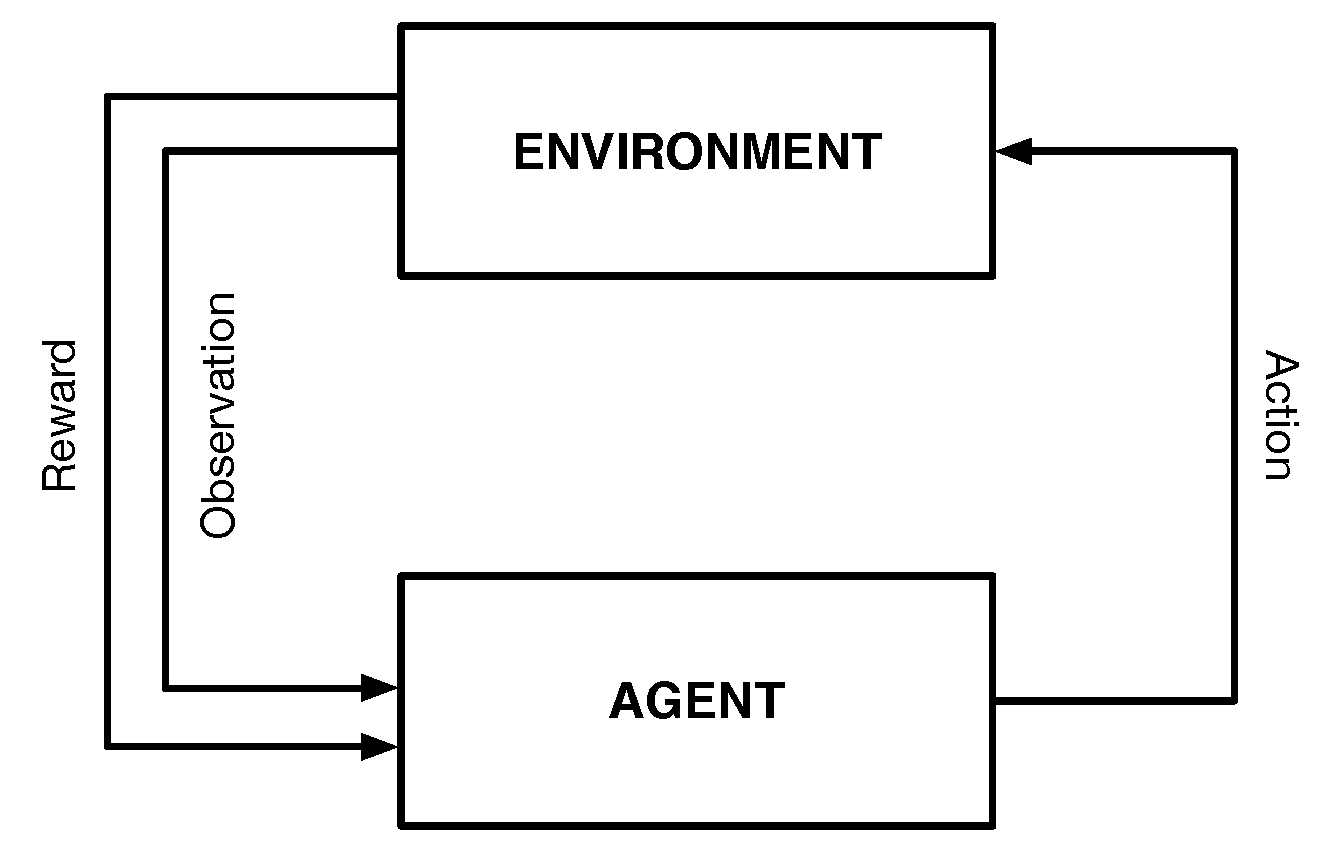
\includegraphics[width=\textwidth]{images/agent-environment.pdf}
\caption{The reinforcement learning process}
\label{fig:agentandenvironment}
\end{figure}
After the action is taken, the state of the environment changes and the agent then receives a new observation of it, and then the process repeats.  The goal of the reinforcement learning agent is to maximize the reward received over a certain time period, finding a balance between immediate and future rewards. 
\end{comment}

Reinforcement learning is an approach to the learning from experience problem in artificial intelligence. A reinforcement learning algorithm's intelligence is built upon having experiences which are then incorporated into the algorithm's own domain knowledge. This knowledge is then used to make intelligent decisions in the future \parencite{barto1998reinforcement}.

\begin{figure}[H]
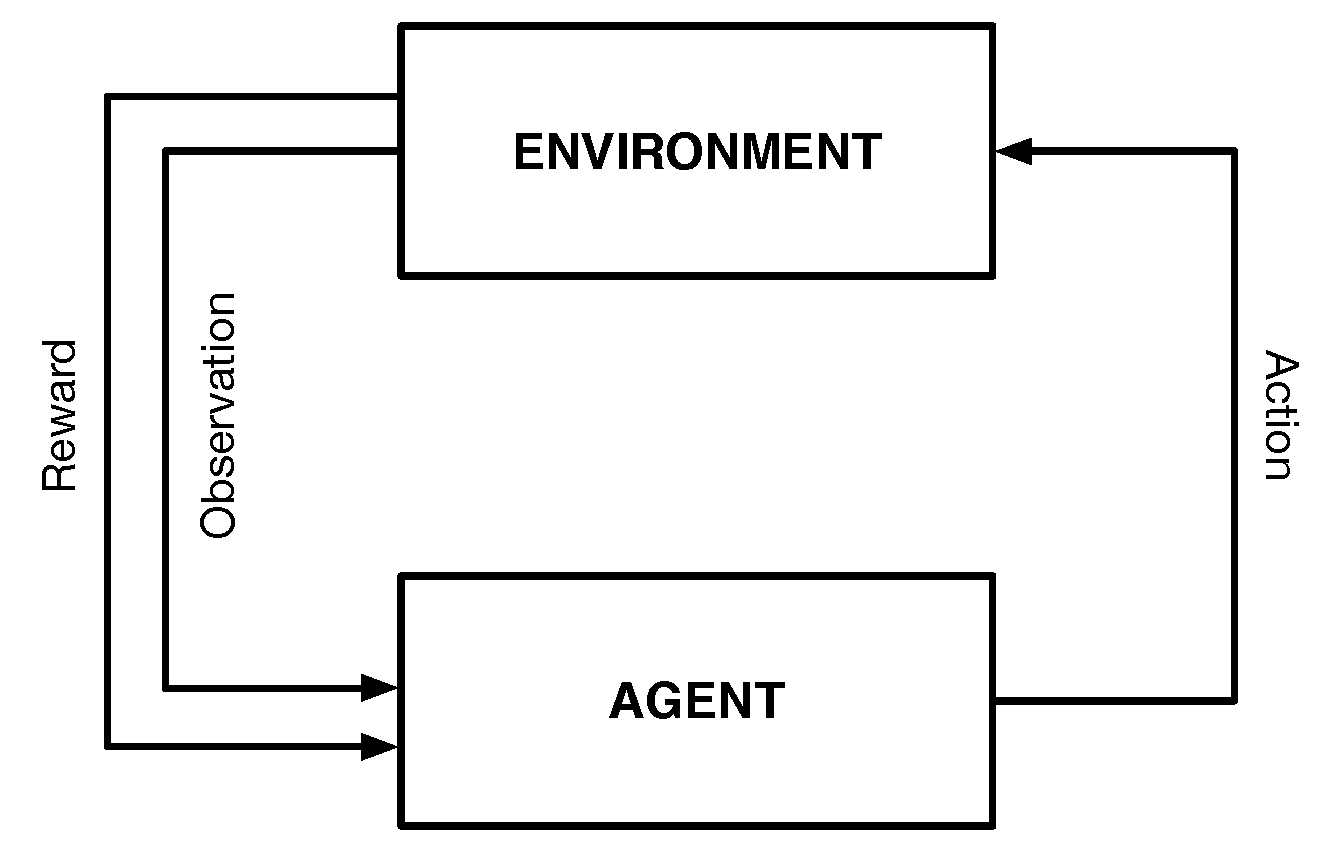
\includegraphics[width=\textwidth]{images/agent-environment.pdf}
\caption{The reinforcement learning process}
\label{fig:agentandenvironment}
\end{figure}

The reinforcement learning problem is modeled as a sequential decision problem, see figure \ref{fig:agentandenvironment} for a graphical representation of the process. A learning algorithm, an agent, performs an action and receives a reward according to some measure of how desirable the results of the action are.  After the action is taken, the state of the environment changes and the agent then receives a new observation of it, and then the process repeats. The goal of the reinforcement learning agent is to maximize the reward received over a certain time period, finding a balance between immediate and future rewards \parencite{barto1998reinforcement}. 


%One thing that sets reinforcement learning apart from other fields within artificial intelligence is that a reinforcement learning problem is solved by an online algorithm. That is, a reinforcement learning algorithm learns about its task and environment while operating in the environment. The actions taken by the agent affect what it knows about the environment, and thus its appraisal of the value of future actions and/or states of the environment.


There are several ways of further dividing reinforcement learning problems into other subcategories. Some examples are the dichotomies 1) episodic/non-episodic problems 2) problems with continuous/discrete state spaces 3) problems with continuous/discrete action spaces 4) problems with one/multiple concurrent agents. (etc.) In the text below, the two first of these dichotomies, which are relevant to this thesis, are discussed. 

\subsection{Episodic and Non-episodic Problems}
One can categorize reinforcement learning problems based on whether or not the time steps are divided into episodes. When the time steps for the agent-environment interaction are divided into subsequences in this manner, the problem is called episodic. This is common in for example games, which end when they are won or lost. If the problem is not episodic, it is called non-episodic, which means, consequently, that the interaction is not divided into subsequences. Instead, the interaction between the actor and environment goes on continually without end \parencite{barto1998reinforcement}. Two examples of non-episodic applications are controlling a robot arm (as well as other robotics problems) and maneuvering a helicopter \parencite{ng2006autonomous}. 

\subsection{Continuous and Discrete Problems}
An alternative way to categorize reinforcement learning problems is based on whether their state spaces are continuous or discrete. An important difference between the two kinds of problems is how an agent can treat similar states in the model. In a continuous problem it is a lot easier to group together states located around the same ``position'' due to the nature of a continuous problem, where the states usually more or less meld together. For example, if the reinforcement learning problem is to control a robot arm whose position is the state of the environment, the different states located around the same general area are not very different. This means that they might be treated in the same way or a similar way by an agent. On the other hand, consider the discrete problem of a game of connect four, wherein the placement of a coin into one of two adjacent slots could dramatically change the evaluation of the state and the outcome of the game \parencite{barto1998reinforcement}.

psection{Markov decision process}

Within reinforcement learning, the concept of Markov secision processes (MDP) is central. An MDP is a way to model an environment where state changes in it are dependent on both random chance and the actions of an agent. An MDP is defined by the quadruple $\left( S, A, P( \cdot , \cdot, \cdot ) , R( \cdot , \cdot ) \right)$ \parencite{altman2002applications}: 

\begin{description}
\item[$S$] \hfill \\ 
    A set of states representing the environment.
\item[$A$] \hfill \\ 
    A set of actions that can be taken.
\item[$P \colon S \times A \times S \to \mathbb R$] \hfill \\ 
    A probability distribution over the transitions in the environment. This function describes the probability of ending up in a certain target state when a certain action is taken from a certain origin state. 
\item[$R \colon S \times A \to \mathbb{R}$] \hfill \\ 
    A function for the reward associated with a state transition. In some formulation of MDPs the reward function only depends on the state.
\end{description}

MDPs are similar to Markov chains, but there are two differences. First, there is a concept of rewards in MDPs, which is absent in Markov chains. Second, in a Markov chain, the only thing that affects the probabilities of transitioning to other states is the current state, whereas in an MPD both the current state and the action taken in that state are needed to know the probability distribution connected with the next state \parencite{altman2002applications}.


\input{Technical_Background/MDP/markov_property.tex}
\input{Technical_Background/MDP/sparse_mdps.tex}
\input{Technical_Background/MDP/factored_representations.tex}


\section{Basic algorithms for solving MDPs}

A policy $\pi$ is a function from a state $s$ to an action $a$ that operates in
the context of a Markov Decision Process, i.e. $\pi \colon S \to A$. A policy
is thus a description of how to act in each state of an MDP. An arbitrary
policy is denoted by $\pi$ and the optimal policy (the policy with the largest
expected reward in the MDP) is denoted by $*$. The rest of this section is
describes some basic algorithms for solving, that is to say finding an optimal
policy, in an MDP.

\subsection{Value functions}

To solve an MDP most algorithms uses an estimation of values of states or
actions. Two value functions are usually defined, the state-value function $V :
S \to \mathbb R$ and the state-action-value function $Q : S \times A \to
\mathbb R$. As the names implies $V$ signifies how good a state is, while $Q$
signifies how good an action in a state is. The state-value function,
$V^\pi(s)$, returns the expected value when starting in state $s$ and following
policy $\pi$ thereafter. Equations \eqref{equation:v_finite} and \eqref{equation:v_infinite} show the equations for the state-value function for a finite time horizon and an infinite, discounted, time horizon respectively. In \eqref{equation:v_infinite}, $\gamma$ is the discount factor, a value between 0 and 1 which describes how fast the value of expected future rewards decay as one looks further into the future. The state-action-value function $Q^\pi(s, a)$ returns
the expected value when starting in state $s$ and taking action $a$ and
thereafter following policy $\pi$. The value functions for the optimal policy
are denoted by $V^*(s)$ and $Q^*(s, a)$. Formulas for the state-action value functions are anologous to those presented for the state value functions. 

\begin{align}
\label{equation:v_finite}
V_t^\pi(s) = \mathbb{E} \{ \sum_{k=0}^{T=k} r_{t+k} | S_t = S, \pi \}
\end{align}

\begin{align}
\label{equation:v_infinite}
V_{0}^\pi(s) = \mathbb{E} \{ \sum_{t=0}^\infty r_{t}\gamma^t | S_0 = S,\pi \}
\end{align}

Both $V^\pi$ and $Q^\pi$ can be estimated from experience. This can be done by
maintaining the average of the rewards that have followed each state when
following the policy $\pi$. When the number of times the state has been
encountered goes to infinity, the average over these histories of rewards
converges to the true values of the value function
\parencite{barto1998reinforcement}.

\input{Technical_Background/ValueFunctions/dynamic_programming.tex}
\input{Technical_Background/ValueFunctions/policy_iteration.tex}
\input{Technical_Background/ValueFunctions/value_iteration.tex}


\subsection{\etre\ in Factored Markov Decision Processes 
\note{N}}
\label{sec:e3_factored_discussion}

\paragraph{General shape of the results} In a comparison of the \etre\ agent's behavior in the different-size environments, the similarity of the shape of the graphs is striking. At first there is a period of lower and lower performance. (For the smallest environments, this period is very short, however.) Next, there is a period of fairly constant high performance, which lasts until the end of the experiment.  

This shape can be explained as a consequence of the different phases of operation of the \etre\ algorithm coupled with the structure of the MDP studied. In the beginning of the experiment, the algorithm will spend almost all of its time in the balanced wandering and exploration phases. The longer the agent has been exploring, and the more states become known, the further the agent has to explore into hard-to-reach parts of the MDP to find unexplored states. Now, in the case of the invasive species environment with the parameters chosen as in the experiments presented, the most easily reachable states are the ones where there is no tamarisk infection. This means that the harder a state is to reach, the more infected it will be, and thus the performance of the \etre\ agent in the exploration phase will fall as the experiment progresses. 

However, once the agent knows enough about the environment to enter the exploitation phase, the \etre\ agent spends close to no time at all exploring unknown states, and it retains high performance. 

\paragraph{Consequences of pooling observation data} An interesting result is that the agent is able to enter the exploitation phase for the 10 reaches/1 habitat per reach test setup slightly earlier than for the 5 reaches/1 habitat per reach setup. This is probably connected to the optimization described in the last paragraph of section \ref{sec:factored_e3}. In the 10 reaches/1 habitat per reach case there are nine reaches with two parents (including the reach itself) and one reach with only itself as parent. In the 5 reaches/1 habitat per reach case there are four reaches with two parents and one reach with only itself as parent. Since observations for state variables with similar parent structure are pooled by our \etre\ implementation, the agent will receive almost double the information per time step for the two-parent reaches in the 10 reaches case as compared to the 5 reaches case.  

\paragraph{Possible issues with the one-policy-per-reach optimization} In section \ref{sec:one_policy_per_state_variable} an optimization is described that works very well for the particular environment and environment settings that the agent was tested for. However, this optimization makes several assumptions that may cause problems if the settings are changed. For instance, one assumption is that the state of a reach is only affected directly by its adjacent parents in the DBN. If the state of a reach was made to depend significantly on other reaches two or more levels up in the river network, the agent would probably not be able to converge on an optimal policy. 

Another assumption that could lead to problems with other environment settings is the assumption that the maximal action cost in the environment is impossible or very hard to break. The invasive species environment has a maximum cost for actions. However, with the standard settings it is mathematically impossible to break this maximum. Our implementation of \etre\ would achieve very poor performance if this was not the case, since a large penalty is given when the maximum action cost is breached. 

\paragraph{DBN structure} Finally, in the invasive species environment, the structure of the DBN underlying the MDP is known at the start of the experiment, so the agent does not need to infer it from its observations. If this was not the case, all the DBN optimizations would be useless unless some kind of algorithm for infering the DBN structure was added to the agent. 

\chapter{Environment and algorithms}
\label{ch:algo}

This chapter gives a description of the environment and the algorithms that
were used in the experiment described in chapter \ref{ch:method}. The environment Invasive Species, is a simulation of a river network with invading species where to goal is to eradicate unwanted species and is further described in section \ref{sec:experiment_env}. 

Two algorithms are covered in this chapter, both of which deal with the
problems that arise with large state spaces; however, they differ in the
methods they apply. In the following chapter the general ideas behind the
algorithms, as well as specific details, are presented. 

The model-based interval estimation algorithm, described in
section~\ref{sec:mbie}, utilizes clever estimations of confidence intervals for
the Q-value functions to improve performance in sparse MDPs.
Section~\ref{sec:fac_e3} is on an algorithm that uses dynamic bayesian networks
and factored representations to improve the \etre\ algorithm to efficiently
deal with factored MDPs. 

\section{Environment specification, Invasive Species}
\label{sec:experiment_env}

When the agents were tested, the Invasive Species environment from the 2014 edition of
the Reinforcement Learning Competition was used. The environment is a
simulation of an invasive species problem, in this case a river network with
invading species where the goal of the agent is to eradicate unwanted species
while replanting native species. 

The environment's model of the river network has parameters, such as the size
of the river network and the rate at which plants spread, which can be
configured in order to create different variations of the environment.  The
size of the river network is defined by two parameters: the number of reaches
and the number of habitats per reach. A habitat is the smallest unit of land
that is considered in the problem. A habitat can either be invaded by the
tamarix, which is an unwanted species, empty or occupied by native species. A
reach is a collection of neighboring habitats. The structure of the river
network is defined in terms of which reach is connected to which
\parencite{invasiveSpecis2014:Online}. In figure \ref{fig:river} a model of a
river network is shown.

\begin{figure}[ht]
\centering
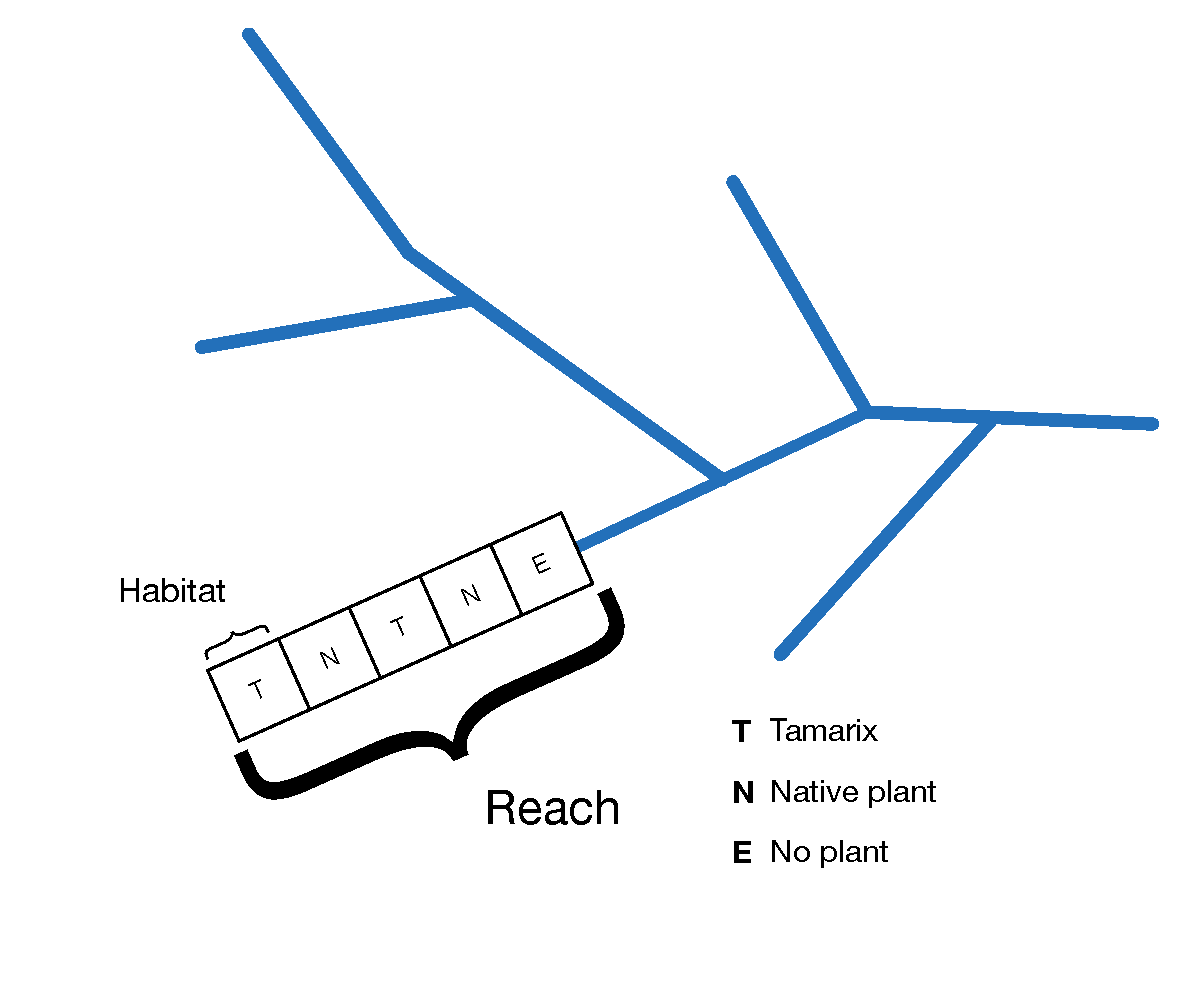
\includegraphics[width=0.9\textwidth]{images/river_network.pdf}
\caption{A river network, as modeled by the Invasive Species reinforcement learning environment.}
\label{fig:river}
\end{figure}

There are four possible actions (eradicate tamarix trees, plant native trees,
eradicate tamarix trees and plant native trees and a wait-and-see action),
and the agent chooses one of these actions for each reach and time step. If the 
agent chooses to eradicate tamarix trees or plant native trees in a reach, 
all habitats of that reach are targeted by this action. What
actions are available to the agent depends on the state of each reach. It is
always possible to choose the wait-and-see action, but there has to be one
or more tamarix-invaded habitats in a reach for the eradicate or eradicate and
plant actions to be available and there has to be at least one empty habitat in
a reach for the plant-native-trees action to be available
\parencite{invasiveSpecis2014:Online}.  

\section{Model-based interval estimation}
\label{sec:mbie}

Model-based interval estimation is a modification of value iteration whose main feature is its  addition of confidence
intervals to the state-action values. These confidence intervals allow the agent to choose between
actions, based on how confident it is about its evaluation of them. In effect,
the less certain the agent is about its evaluation of the states and actions,
the more exploratory the actions will be. When the agent is more confident
however, it will exploit what it has learnt so far about the MDP
\parencite{dietterich2013pac}.

\input{algorithms/MBIE/modification_of_value_it}
\input{algorithms/MBIE/gt.tex}
\input{algorithms/MBIE/modded_bounds}

\section{\etre\ in factored Markov decision processes}
\label{sec:fac_e3}

The second algorithm studied in this thesis is a version of the \etre\ algorithm that focuses on factored problem domains by modeling them as a dynamic Bayesian network. The original \etre\ algorithm is described in section \ref{sec:e3}, which gives a broad overview along with the key strategies used in the algorithm. The following section, \ref{sec:factored_e3}, considers some ways to extend the original algorithm and make use of factored representations and planning in factored domains to improve the running time of the algorithm.

\input{algorithms/Factored_E3/e3.tex}
\input{algorithms/Factored_E3/factored_additions.tex}


\chapter{Method}
\label{sec:method_intro}

This chapter covers the preliminaries and preparations carried out before the
execution of the experiments. It covers  and how the agents described in chapter
\ref{ch:algo} were implemented and the additions and modifications that were made to them. The chapter
concludes with a description of the tools used for the experiment.
\section{Algorithm implementation}
\label{sec:implementation}

We implemented two existing algorithms and we also added some extensions.  The
experiment utilized RL-Glue (section~\ref{sec:rl_glue}) to connect the agents
and environment to each other.  To verify the behavior of our agents we utilized smaller
environments (see sections~\ref{sec:intro_grid_world} and \ref{sec:ns}) where
the correct operation is either easy to derive or obvious from inspection. By
starting with smaller problems and using an iterative approach it was possible
to identify bottlenecks in our implementations and correct possible errors
early.

\input{algorithms/MBIE/modded_bounds}

\input{method/ConstructingExperiments/contributionse3}

\subsection{GridWorld}
\label{sec:intro_grid_world}

The GridWorld environment was implemented to easily be able to verify the
correctness of the MBIE algorithm. It consists of a grid of twelve squares with
one blocked square, one starting square, one winning square, one losing square and
eight empty squares. The agent can take five actions, north, south, west,
east or exit. The exit-action is only possible from the winning or losing
state. When taking an action being in one state and the action is directed to
another empty state there is an 80\% probability to succeed and 10\%
probability to fail and 10\% to go sideways.

\subsection{Network simulator}
\label{sec:ns}

A simple computer network simulation was implemented to verify the behavior of an
early version of \etre\ algorithm. In this environment, the agent tries to keep
a network of computers up and running. All computers start in the running
state, but there is a chance that they randomly stop working. If a computer is
down, it has a chance to cause other computers connected to it to also fail. In
each time step, the agent chooses one computer to restart, which with 100
percent probability will be in working condition in the next time step. The
agent is rewarded for each computer in the running state after each time step. 

\section{Our contributions}
\label{sec:contributions}


\input{algorithms/MBIE/modded_bounds}


\input{method/ConstructingExperiments/contributionse3}

\section{Environment specification}
\label{sec:experiment_env}

For the experiment, the Invasive Species environment from the 2014 edition of
the Reinforcement Learning Competition was used. The environment is a
simulation of an invasive species problem, in this case a river network with
invading species where the goal of the agent is to eradicate unwanted species
while replanting native species. 

The environment's model of the river network has parameters, such as the size
of the river network and the rate at which plants spread, which can be
configured in order to create different variations of the environment.  The
size of the river network is defined by two parameters: the number of reaches
and the number of habitats per reach. A habitat is the smallest unit of land
that is considered in the problem. A habitat can either be invaded by the
tamarix, which is an unwanted species, empty or occupied by native species. A
reach is a collection of neighboring habitats. The structure of the river
network is defined in terms of which reach is connected to which
\parencite{invasiveSpecis2014:Online}. In figure \ref{fig:river} a model of a
river network is shown.

\begin{figure}[ht]
\centering
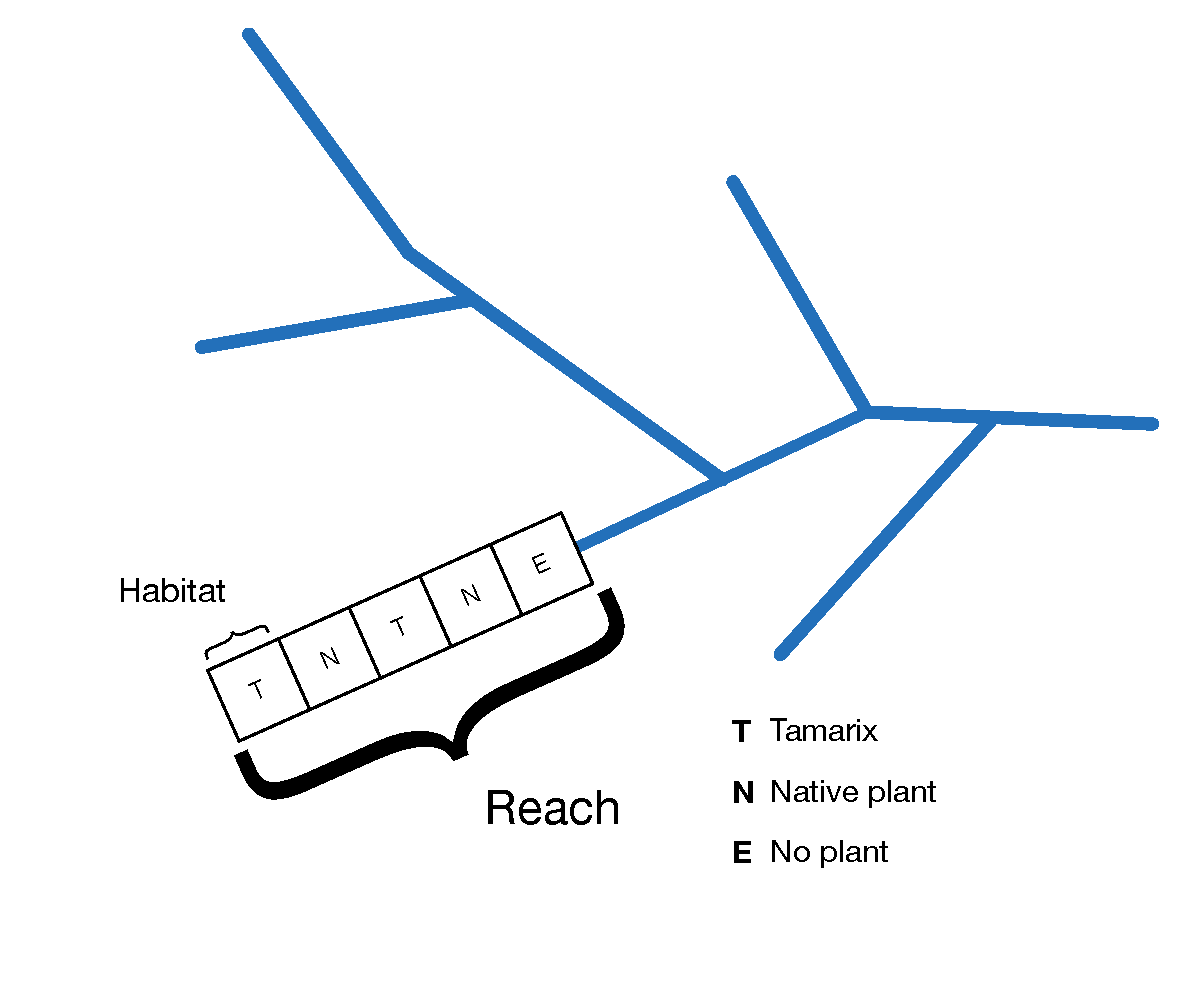
\includegraphics[width=0.9\textwidth]{images/river_network.pdf}
\caption{A river network, as modelled by the Invasive Species reinforcement learning environment.}
\label{fig:river}
\end{figure}

There are four possible actions (eradicate tamarisks, plant native trees,
eradicate tamarisks and plant native trees, and finally a wait-and-see action),
and the agent chooses one of these actions per reach per time step. What
actions are available to the agent depends on the state of each reach. It is
always possible to choose the wait-and-see action, but there has to be one
or more tamarix-invaded habitats in a reach for the eradicate or eradicate and
plant actions to be available and there has to be at least one empty habitat in
a reach for the plant-native-trees action to be avalable
\parencite{invasiveSpecis2014:Online}. 

\section{Test specification}
\label{sec:test_spec}

The testing of the agents required us to choose certain sets of parameters, for
the environment, the two different agents and the experiment itself. 

\paragraph{Environment parameters}

The Invasive Species environment requires a number of parameters. For further
explanation of the environment parameters consult the environment
webpage\footnote{\url{http://2013.rl-competition.org/domains/invasive-species}}.
The specific parameters used are presented in
appendix~\ref{ap:environment_spec}.

\paragraph{Agent Parameters}

The agents evaluated required different types of parameters. Some preliminary
tests were run and then the parameters giving best results were chosen.
Parameters for MBIE are found in table~\ref{tab:mbie_params_both}.

\begin{table}[H]
\centering
\captionof{table}{Parameters for MBIE}
\label{tab:mbie_params_both}

\begin{subfigure}[b]{0.47\textwidth}
    \centering
    \captionof{table}{Proper MBIE}
    \label{tab:mbie_params} 
    \begin{tabular}{lr}
     \toprule
     Parameter & Value \\
     \midrule
     Discount factor, $\gamma$ & 0.9 \\
     Confidence, $\delta$ & 95\% \\
     $\Delta \omega$ & $\frac{1}{2}\sqrt{\frac{2|ln(2^{|S|}-2) - ln  \delta |}{N(s,a)}}$ \\
     
     \bottomrule
    \end{tabular}
\end{subfigure}
\quad
\begin{subfigure}[b]{0.47\textwidth}
    \centering
    \captionof{table}{Realistic MBIE}
    \label{tab:mbie_realistic_params}
    \begin{tabular}{lr}
     \toprule
     Parameter & Value \\
     \midrule
     Discount factor, $\gamma$ & 0.9 \\
     $\Delta \omega$ & $1 - 0.05 N(s,a)$ \\
     \bottomrule
    \end{tabular}
\end{subfigure}
\end{table}

For DBN-\etre\ a higher exploration limit resulted in the agent starting to
exploit earlier but with a slightly lower final return. A higher partial state
known limit resulted in later exploitation but no appreciable difference in
final return. The values in table~\ref{tab:dbne3_params} were a good middle
ground.

\begin{table}[H]
\captionof{table}{DBN-\etre\ parameters}
\label{tab:dbne3_params}
\centering
\begin{tabular}{lr}
 \toprule
 Parameter & Value \\
 \midrule
 Discount factor & 0.9 \\
 Exploration limit & 5\% \\
 Partial state known limit & 5 \\
 \bottomrule
\end{tabular}
\end{table}

\paragraph{Experiment parameters}

The tests performed had to be long enough to sample enough data to extract
relevant results without making the running time too long. A single test
consisted of a specific number of episodes with a specific length. A good
combination was required to efficiently evaluate the agents. If a single
episode consisted of too many samples it would be difficult to see the learning
process as results are reported as total reward over an episode and that
process might be hidden as its impact on the total reward is smaller with a
longer episode. On the other hand, if an episode length is too short it would
end before the agents could do any valuable learning.

In addition to a satisfactory episode length, a reasonable number of episodes
needs to be sampled for it to be possible to draw conclusions from the results.
If the number of episodes is too small, the convergence of the agents cannot be
seen. However, if the number of episodes are too large a lot of sampled data
would be redundant for the study. Some preliminary experiments were run in
order to tune the experiment parameters to suitable values. The episode length
was set to 100 samples and there were 100 episodes per test.

To evaluate the agents in the Invasive Species environment combinations of
reaches and number of habitats per reach that can be seen in
table~\ref{tab:reaches_habitats} were choosen. Combinations were chosen to have
a wide range in the total number of states for the agents to deal with and to
test how the agents deal with taking actions that have to take into account
several state components. 

As seen in table ~\ref{tab:reaches_habitats}, the state count increases rapidly
when habitats are added to the problem. This is obvious from the fact that the state count
depends exponentially on the total number of habitats; see equation \eqref{eq:statecount}, where $h$ is the number of habitats per reach and $r$ is the number of reaches.

\begin{equation}
\label{eq:statecount}
 |S| = 3 ^ {hr}
\end{equation}

\begin{table}[H]
\centering
\caption{Combinations of reaches and habitats used in testing.}
\label{tab:reaches_habitats}
\begin{tabular}{rrr}
 \toprule
 Reaches & Habitats per reach & Total state count \\
 \midrule
 5  & 1 &          243 \\
 3  & 2 &          729 \\
 3  & 3 &      19\,683 \\
 10 & 1 &      59\,049 \\
 4  & 3 &     531\,441 \\
 5  & 3 & 14\,348\,907 \\
 \bottomrule
\end{tabular}
\end{table}

\section{Programming environment}
\label{sec:prog_env}

The Java programming language 1.7 was used to implement the algorithms. In addition, the
Java version of RL-Glue framework version 3.0 was used. For version control Git
was used, due to its simplicity and performance.

\section{RL-Glue}
\label{sec:rl_glue}

To evaluate the agents the RL-Glue framework was used, which acts as an
interface for communication between the agent and the environment. The software
uses the RL-Glue protocol, which specifies how a reinforcement learning problem
should be divided when constructing experiments and how the different programs
should communicate \parencite{tanner2009rl}.

RL-Glue divides the reinforcement learning process into three separate
programs: an agent, an environment and an experiment. RL-Glue provides a server
software that manages the communication between these programs. The agent and
the environment programs are responsible for executing the tasks as specified
by RL-Glue and the experiment program acts as a bridge between the agent and
environment \parencite{tanner2009rl}.

The modular structure of RL-Glue makes it easier to construct repeatable
reinforcement learning experiments. By separating the agent from the
environment it is possible to reuse the environment and switch out the agent.
It also makes it a lot easier to cooperate and continue working on existing
environments implemented by other programmers.


\chapter{Result}

\newcommand{\graphwidth}{0.70\textwidth}
\newcommand{\testsubfigure}[2]{%
\begin{subfigure}[b]{\graphwidth}
    \includegraphics[width=1.1\textwidth]{images/tests/#1r-#2h.pdf}
    \caption{#1 reaches and #2 habitats per reach}
    \label{fig:#1r#2h}
\end{subfigure}
}

In figures~\ref{fig:tests1}, \ref{fig:tests2} and \ref{fig:tests3} we have test results from running our agents on the invasive species environment on different sizes of river network. The raw data can be found in appendix~\ref{ap:result_tables}.

\begin{figure}[h!]
    \centerline{
    \testsubfigure{3}{3}
    ~
    \testsubfigure{3}{2}
    }
    \caption{Test runs with different number of reaches and habitats}
    \label{fig:tests1}
\end{figure}

\begin{figure}[h!]
    \centerline{
    \testsubfigure{5}{1}
    ~
    \testsubfigure{5}{3}
    }
    \caption{Test runs with different number of reaches and habitats}
    \label{fig:tests2}
\end{figure}

\begin{figure}[h!]
    \centerline{
    \testsubfigure{4}{3}
    ~
    \testsubfigure{10}{1}
    }
    \caption{Test runs with different number of reaches and habitats}
    \label{fig:tests3}
\end{figure}

The agent learns for 100 episodes with 100 samples per episode, other parameters are specified in section~\ref{sec:test_spec}. The invasive species environment associates a certain cost with each state and action, thus the reward is always negative. In each test the reward varies over time for the MBIE agent, the realistic MBIE agent and the DBN-\etre\ agent.

With smaller state spaces (see figure~\ref{fig:3r3h}, \ref{fig:3r2h} and \ref{fig:5r1h}) we can see that the realistic MBIE agent outperforms the proper MBIE agent and comes close to the DBN-\etre\ agent. In the tests where the state space is larger (see figure~\ref{fig:5r3h}, \ref{fig:10r1h} and \ref{fig:4r3h}) proper MBIE and realistic MBIE are very close to each other in performance while the DBN-\etre\ agent outperforms both. The realistic MBIE algorithm performs better in with smaller state spaces due to more states becoming known quicker and thus having their true value.

In each of the test runs the DBN-\etre\ algorithm exhibits a period of learning that corresponds to exploration (as described in section~\ref{sec:e3}) where the agent has not explored the environment enough and seeks more information. This is apparent in figure~\ref{fig:3r3h}.
\chapter{Discussion \note{B}}
\label{ch:discussion}
This chapter is a discussion of the results and method used in the project. The algorithms are evaluated with regard to their performance achieved in the tests, which is used as a basis when comparing them against each-other. Determining their strengths and weaknesses and if they were suitable for problems with an environment that has a large discrete state space and in particular for the environment Invasive Species. There is also a discussion on ethical aspects regarding the work in this thesis.


% Det behövs inte en ingående disposition här, det tar ner läsligheten. Det som tas upp i styckena är vettigt, men detta är inte rätt ställe för dem.

% This chapter is a combination of discussion of the results of using the algorithms described in chapter \ref{ch:algo}, together with a examination of the method used in the project. The algorithms is evaluated with regard to their performance achieved in the experiments \ref{sec:constructing_experiments}, which is used for a basis when comparing them against each-other. Focusing on their strengths and weaknesses and circling around the question why did they perform as they did. Were they suitable for this kind of problem, an environment with a large discrete state space and in particular for this thesis a simulation of an Invasive Species environment.

% The second part of this chapter contains a section containing a presentation of similar studies conducted, summarizing their results and opinions. Using their finding as a basis, there will also be a discussion regarding its connection to the results in this thesis. With inspiration from similar studies in combination with the results of this thesis, a discussion about the possible extensions and additional work or unanswered questions in this thesis are presented. 

%In order to round of this chapter, the last section of this chapter revolves around ethical questions and aspects regarding the theme of this topic. The main theme of the last section is ethical aspects in \acrlong{ai} \acrshort{ai}, \acrfull{ai}, along with a discussion about the usefulness of Reinforcement Learning in today's society with focus on using simulations.

\section{Evaluation of the agents \note{I}}
\label{sec:coa}

\input{Discussion/AlgorithmsEvaluation/dbn.tex}
\input{Discussion/AlgorithmsEvaluation/mbie.tex}
\input{Discussion/AlgorithmsEvaluation/discussion_diffrences}




\section{Potential factors impacting the results}
\label{sec:truth_results}

There are several factors that possibly reduce the reliability of the results. For instance, all evaluations used only one environment, the implementation of the algorithms could contain errors and the correct results for all test runs are not always known. 

\input{Discussion/discussion_results/impact_of_one_env.tex}

\input{Discussion/discussion_results/implementation_of_algorithms.tex}

\input{Discussion/discussion_results/testing_methodology.tex}


%\section{Similar Studies \note{N, K}}
The work with reducing the complexity of the reinforcement learning problems with environments containing large state spaces is not a new research topic. However, this thesis is taking a rather uncommon approach to the problem. Instead of trying to derive new algorithms for solving the problem, the focus is instead focused on usefulness of research conducted within the area of reinforcement learning problems. To be even more specific this thesis has zoomed in on two possible attempts on solving the problem with environments containing large state spaces. An approach that is rather uncommon and thus similar studies is as well uncommon. 
%Behöver skrivas om, tydligare
Thereby this section will combining focus on both studies similar to this thesis comparing the usefulness of research already conducted along with a summarized study of studies of work being done to reduce the complexity of environments with large state spaces.

\todo[inline]{Samma miljö kanske, dess pac?}

\paragraph{Similar Studies Regarding Comparing Existing Research}
\todo[inline]{Borde finnas återkoppling i diskussion kring detta}
It has been shown in Strehl and Littman (2004; 2008) that MBIE outperforms \etre\ in the MDPs RiverSwim and SixArms. \parencite{dietterich2013pac}


\paragraph{Large State Spaces using Dynamic Bayesian Networks}
This paragraph is devoted to similar methods using dynamic Bayesian networks as an underlying representation in order to model the structure of the environment. Due to the relevance of using dynamic Bayesian network as a method for tackling similar problems it is thesis on its own in order to summarize them all. It is also possible to study section \ref{sec:better_planing_algos} for further references, however their main focus on the planning algorithm.

An algorithm to DBN-\etre\ is the algorithm by \textcite{ross2012model} which is as well utilizing a factored representation for the underlying structure. However, in the DBN-\etre\ algorithm no planning algorithm was specified and therefore leaving an empty square in the implementation affecting the overall complexity of the algorithm. In the algorithm by \textcite{ross2012model} 

\todo[inline]{Resultatjämförelse}

\paragraph{Similar Studies Regarding Large State Spaces Using Model Based Something grejen}
Grattis MBIE, er punkt.

\section{Ethical and social aspects of artificial intelligence}

\input{Discussion/Ethics/intro.tex}

\input{Discussion/Ethics/invasive_species.tex}

\input{Discussion/Ethics/ai_right_or_wrong.tex}



\section{Further work}

In this section we discuss possible further work and extensions to our thesis.

\input{Discussion/further_work/more_test_envs.tex}
\input{Discussion/further_work/better_planning_dbn.tex}
\input{Discussion/further_work/MBIE.tex}
\input{Discussion/further_work/mbie_should_use_dbn.tex}


\printbibliography

\begin{appendices}

\chapter{Environment specification}
\label{sec:environment_spec}

\begin{table}[H]
\centering
\captionof{table}{Dynamic parameters common to both species}
\label{tab:dynamic_params_common} 
\begin{tabular}{l r}
 \toprule
 Parameter & Value \\
 \midrule
 Eradication rate & 0.85 \\
 Restoration rate & 0.65 \\
 Downstream spread rate & 0.5 \\
 Upstream spread rate & 0.1 \\
 \bottomrule
\end{tabular}
\end{table}

\begin{table}[H]
\centering
\captionof{table}{Dynamic parameters different between the species} \label{tab:dynamic_params_not_common}
\begin{tabular}{lrr}
\toprule
 Parameter & Native & Tamarisk \\
 \midrule
 Death rate & 0.2 & 0.2 \\
 Production rate & 200 & 200 \\
 Exogenous arrival\footnote{Arrival of seeds from outside the environment} & Yes & Yes \\
 Exogenous arrival probability & 0.1 & 0.1 \\
 Exogenous arrival number & 150 & 150 \\
 \bottomrule
\end{tabular}
\end{table}

\begin{table}[H]
\centering
\captionof{table}{Cost function parameters} \label{tab:cost_params} 
\begin{tabular}{lr}
 \toprule
 Parameter & Value \\
 \midrule
 Cost per invaded reach & 10 \\
 Cost per tree & 0.1 \\
 Cost per empty slot & 0.01 \\
 Eradication cost & 0.5 \\
 Restoration cost & 0.9 \\
 \bottomrule
\end{tabular}
\end{table}

\begin{table}[H]
\centering
 \captionof{table}{Variable costs depending on number of habitats affected by action}
 \begin{tabular}{lr}
 \toprule
 Parameter & Value \\
 \midrule
 Eradication cost & 0.4 \\
 Restoration cost for empty slot & 0.4 \\
 Restoration cost for invaded slot & 0.8 \\
 \bottomrule
\end{tabular}
\label{tab:cost_params_var}
\end{table}
\end{appendices}


\end{document}

\RequirePackage[l2tabu,orthodox]{nag}

\documentclass[bachelors,a4paper]{chalmers-thesis}

\usepackage[swedish, english]{babel}

\usepackage[utf8]{inputenc}
\usepackage{comment}
\usepackage{color}
\usepackage{todonotes}
\usepackage{hyperref}


% To be able to include pdfs in the document
\usepackage{pdfpages}

% To use appendices
\usepackage[toc,page]{appendix}

% Fancy maths!
\usepackage{amsmath}
\usepackage{amssymb}

% Fancy references
\usepackage[style=authoryear,date=iso8601]{biblatex}
\addbibresource{jelzin.bib}

% Fancy graphics
\usepackage{graphicx}

% For the finest tables
\usepackage{booktabs}
\usepackage{longtable}

% For mutliple column pages
\usepackage{multicol}

% For the finest of subfigures in figures or tables
\usepackage{subcaption}

% To be able to position figure envs exactly where you want them use H.
\usepackage{float}

% Nice environments for pseudocode
\usepackage[chapter]{algorithm}
\usepackage{algpseudocode}

\title{Reinforcement learning}
\subtitle{A comparison of learning agents in environments with large discrete state spaces}
\author{%
Johan Andersson\and
Emil Kristiansson\and
Joakim Persson\and
Adam Sandberg Eriksson\and
Daniel Toom\and
Joppe Widstam}
\thesisin{Computer Science}
\department{Department of Computer Science and Engineering}
\reportno{2014:05}
\copyrightyear{2014}
\keywords{Reinforcement learning, Artificial intelligence, MBIE, DBN-\etre, Invasive Species, Learning algorithms}

% Abstracts
\firstabstract{% 1 Motivation

For some real-world behavior optimization problems, it is infeasible to search for a solution by making a model of the problem and performing calculations on it. 
In cases like these, good solutions can sometimes be found by trial and error. 
Reinforcement learning is a way of finding optimal behavior by systematic trial and error.
% 2 Problem statement
This thesis aims to compare different reinforcement learning techniques and evaluate them. 
Model-based interval estimation (MBIE) and Explicit explore or exploit using dynamic bayesian networks - (DBN-\etre)
 are two algorithms that are evaluated. 
% 3 Approach
To evaluate the techniques, learning agents were constructed using the algorithms and 
then simulated in the environment invasive species from the reinforcement learning competition.
% 4 Results
The results of the study show that an optimized version of DBN-\etre\ is better than MBIE at finding an optimal or near optimal behavior policy in the 
environment invasive species for a selection of environment parameters.

% 5 Conclusions
Using a factored model like a DBN shows certain advantages operating in 
the factored environment invasive species. For example it achieves a near optimal
policy within fewer episodes than MBIE.


% Följande saker ska vara med i en abstract Motivation, Problem Statement, Approach, REsults

% Motivation
% Why do we care about the problem and the results? 
% If the problem isn't obviously "interesting" it might be better to
% put motivation first; but if your work is incremental progress on
% a problem that is widely recognized as important, then it is 
% probably better to put the problem statement first to indicate which
%  piece of the larger problem you are breaking off to work on.
% This section should include the importance of your work, the difficulty
% of the area, and the impact it might have if successful.

% Problem statement
% What problem are you trying to solve? What is the scope of your work 
%(a generalized approach, or for a specific situation)? Be careful not to 
% use too much jargon. In some cases it is appropriate to put the problem 
% statement before the motivation, but usually this only works if most 
% readers already understand why the problem is important.

% Approach
% How did you go about solving or making progress on the problem? Did you 
% use simulation, analytic models, prototype construction, or analysis of
% field data for an actual product? What was the extent of your work
% (did you look at one application program or a hundred programs in
% twenty different programming languages?) What important variables did
% you control, ignore, or measure?

% Results
% What's the answer? Specifically, most good computer architecture papers 
% conclude that something is so many percent faster, cheaper, smaller, 
% or otherwise better than something else. Put the result there, in
% numbers. Avoid vague, hand-waving results such as "very", "small",
% or "significant." If you must be vague, you are only given license
% to do so when you can talk about orders-of-magnitude improvement. 
% There is a tension here in that you should not provide numbers that
% can be easily misinterpreted, but on the other hand you don't have
% room for all the caveats.

% Conclusions
% What are the implications of your answer? Is it going to change the 
% world (unlikely), be a significant "win", be a nice hack, or simply 
% serve as a road sign indicating that this path is a waste of time 
% (all of the previous results are useful). Are your results general, 
% potentially generalizable, or specific to a particular case?
}
\secondabstract{swedish}{% 1 Motivation
För vissa verklighetsbaserade optimeringsproblem där det gäller att finna ett bästa beteende är det orimligt söka efter det optimala beteendet genom att skapa en modell av problemet och sedan utföra beräkningar på den. I vissa sådana fall kan man hitta bra lösningar genom trial and error. Reinforcement learning är ett sätt att hitta optimalt beteende genom att systematisk pröva sig fram.
% 2 Problem statement
Detta kandidatarbete har som mål att jämföra olika inlärningstekniker och utvärdera dessa.
Model-based interval estimation (MBIE) och Explicit Explore or Exploit med dynamiska bayesnät (DBN-\etre) är 
två självlärande algoritmer som här utvärderas.

% 3 Approach
För att utvärdera de olika teknikerna implementerades agenter som använde algoritmerna, och dessa testkördes sedan 
i miljön invasive species från tävlingen Reinforcement learning competition.

% 4 Results
DBN-\etre\ är bättre än MBIE på att hitta en optimal eller nära optimal policy i miljön invasive species med valda parametrar.
% 5 Conclusions
Att använda en faktoriserad model, så som DBN-\etre\, visar på tydliga fördelar i faktoriserade miljöer, som i till exempel invasive species. 
Ett exempel på detta är att den når en nästan optimal policy på färre episoder än MBIE.

% Följande saker ska vara med i en abstract Motivation, Problem Statement, Approach, REsults

% Motivation
% Why do we care about the problem and the results? 
% If the problem isn't obviously "interesting" it might be better to
% put motivation first; but if your work is incremental progress on
% a problem that is widely recognized as important, then it is 
% probably better to put the problem statement first to indicate which
%  piece of the larger problem you are breaking off to work on.
% This section should include the importance of your work, the difficulty
% of the area, and the impact it might have if successful.

% Problem statement
% What problem are you trying to solve? What is the scope of your work 
%(a generalized approach, or for a specific situation)? Be careful not to 
% use too much jargon. In some cases it is appropriate to put the problem 
% statement before the motivation, but usually this only works if most 
% readers already understand why the problem is important.

% Approach
% How did you go about solving or making progress on the problem? Did you 
% use simulation, analytic models, prototype construction, or analysis of
% field data for an actual product? What was the extent of your work
% (did you look at one application program or a hundred programs in
% twenty different programming languages?) What important variables did
% you control, ignore, or measure?

% Results
% What's the answer? Specifically, most good computer architecture papers 
% conclude that something is so many percent faster, cheaper, smaller, 
% or otherwise better than something else. Put the result there, in
% numbers. Avoid vague, hand-waving results such as "very", "small",
% or "significant." If you must be vague, you are only given license
% to do so when you can talk about orders-of-magnitude improvement. 
% There is a tension here in that you should not provide numbers that
% can be easily misinterpreted, but on the other hand you don't have
% room for all the caveats.

% Conclusions
% What are the implications of your answer? Is it going to change the 
% world (unlikely), be a significant "win", be a nice hack, or simply 
% serve as a road sign indicating that this path is a waste of time 
% (all of the previous results are useful). Are your results general, 
% potentially generalizable, or specific to a particular case?
}

% Useful commands
\newcommand{\note}[1]{\textcolor{red}{#1}}
\newcommand{\etre}{\ensuremath{E^3}}

\begin{document}

\makecoverpage
\maketitlepage
\makeprintinfopage

\newpage

\pagenumbering{roman}
\pagestyle{plain}

\makeabstractpage
\makesecondabstractpage

\newpage

\tableofcontents

\newpage

\pagenumbering{arabic}

\chapter{Introduction}
\label{sec:intro_intro}

This thesis evaluates and compares two existing algorithms and therefore it has
negliable impact on matters such as ethics, social or economics in today's
society. Therefore this sections focuses on the futher impact of artificial
intelligence using models of the real world and simulations along with a
high-level discussion regarding right or wrong with artificial intelligence.
\section{Purpose and problem statement}

This thesis aims to further the knowledge of reinforcement learning or more specifically, algorithms applied to reinforcement learning problems with large state spaces. Reinforcement learning algorithms struggle with environments consisting of large state spaces due to practical limitations in memory usage and difficulties in estimating the value of actions and states within reasonable processing time. Therefore, we aim to evaluate techniques to circumvent or reduce the impact of these limitations by implementing algorithms using these techniques and testing and comparing them on problems of different sizes.


\section{Limitations \note{Ny Text}}
\label{sec:discuss_limitations}
In section \ref{sec:limitations}, the limitations for the project were stated and besides the fact that this thesis focuses environments with large state spaces. In order for the results from testing the algorithms selected to be relevant, the choice of environment is significant. The information gathering process during the pre-study was a more complex process than expected. The clear limitation of environment phases reduced the overall complexity with the reinforcement learning field and served as a great way to narrow the field of study. Without the reduction of the potential open research areas in reinforcement learning by first selecting the problem type and a corresponding environment the project would have become significant arduous to manage and execute. 

Nevertheless, there is also a different aspect of making an early choice of environment and problem area. The early decision of environment could possibly have eliminated algorithms from other fields in reinforcement learning which could have yielded superior results than the results collected in this project. Although, given the circumstances of the project, a delay in the choice of environment only could have lead to time spent wasted and perhaps resulted in a direction of the project not leading to any significant results at all. 

Because some papers do not include proper testing, it is possible that a algorithm only works in theory due to limitations with today computers computational power and memory. Another reason behind focusing on open research topics is on the grounds that the group lacks extensive background in the reinforcement learning field and have an desire to start working with practical issues rather than spending all the time in the beginning of the project reasoning about algorithms strength and weakness first handed. Instead focusing on combining the study of reinforcement learning in general and bringing two selected agents to life, the learning outcome has been maximized and as the project matured the knowledge and understanding of the subject also matured making it easier to reason about the qualities of the algorithms and also find areas where optimizations can be applied. 
\section{Simulation environment}
\label{sec:env_used}
The environment used is invasive species from the Reinforcement Learning Competition, described in section \ref{sec:experiment_env}. Depending on the parameters, the problem can have both a large state space and/or a large action space. This makes invasive species a good choice with the given problem statement.


\section{Agents to be Evaluated}
Two algorithms that are suitable to the purpose and problem statement, since they apply different techniques for working with large state spaces, are Explicit Explore or Exploit in Dynamic Bayesian Networks (DBN-\etre) and Model Based Interval Estimation (MBIE). They are described in detail in chapter \ref{ch:algo}. 





% tests using these algorithms should yield interesting data to be used for the evaluating the two agents and compare them against each-other. 
\chapter{Technical background}
This chapter is for readers new to the reinforcement learning area. A short overview is first given of artificial intelligence and how reinforcement learning fits within the field of artificial intelligence, the chapter then continues with the main topics and concepts necessary to understand the rest of the report. 

% This technical background has a theoretical outlook and in some cases discusses the mathematical background.

%This technical background has a slightly more theoretical outlook and in some cases discusses more of the mathematical background than the introduction given in chapter \ref{sec:intro_intro}. 

The term artificial intelligence was coined by John McCarthy who described it as ``the science and engineering of making intelligent machines'' \parencite{McCarthy2007:Online}. More specifically, it addresses creating intelligent computer machines or software that can achieve specified goals computationally. These goals can comprise anything, e.g. writing poetry, playing complex games such as chess or diagnosing diseases. Different branches of artificial intelligence include planning, reasoning, pattern recognition and the focus of this thesis: learning from experience.
This chapter gives a more formal description of reinforcement learning and the main topics and concepts necessary to understand the rest of the report. 


\section{Reinforcement Learning \note{Reviderad}}

%These areas comprise different subcategories and problems of their own. An approach to learning from experience is Reinforcement Learning, where the agent takes an action and receives a reward according to some measure of how good the action was. This could be compared to Pavlovian conditioning: teaching dogs by rewarding them for desired behavior and punishing them for undesired behavior. 

\begin{comment}
Reinforcement learning is an approach to the learning from experience problem in artificial intelligence. The reinforcement learning problem is modeled as a sequential decision problem: a learning algorithm, an agent, performs an action and receives a reward according to some measure of how desirable the results of the action are. See figure \ref{fig:agentandenvironment} for a graphical representation of the process \parencite{barto1998reinforcement}.
\begin{figure}[H]
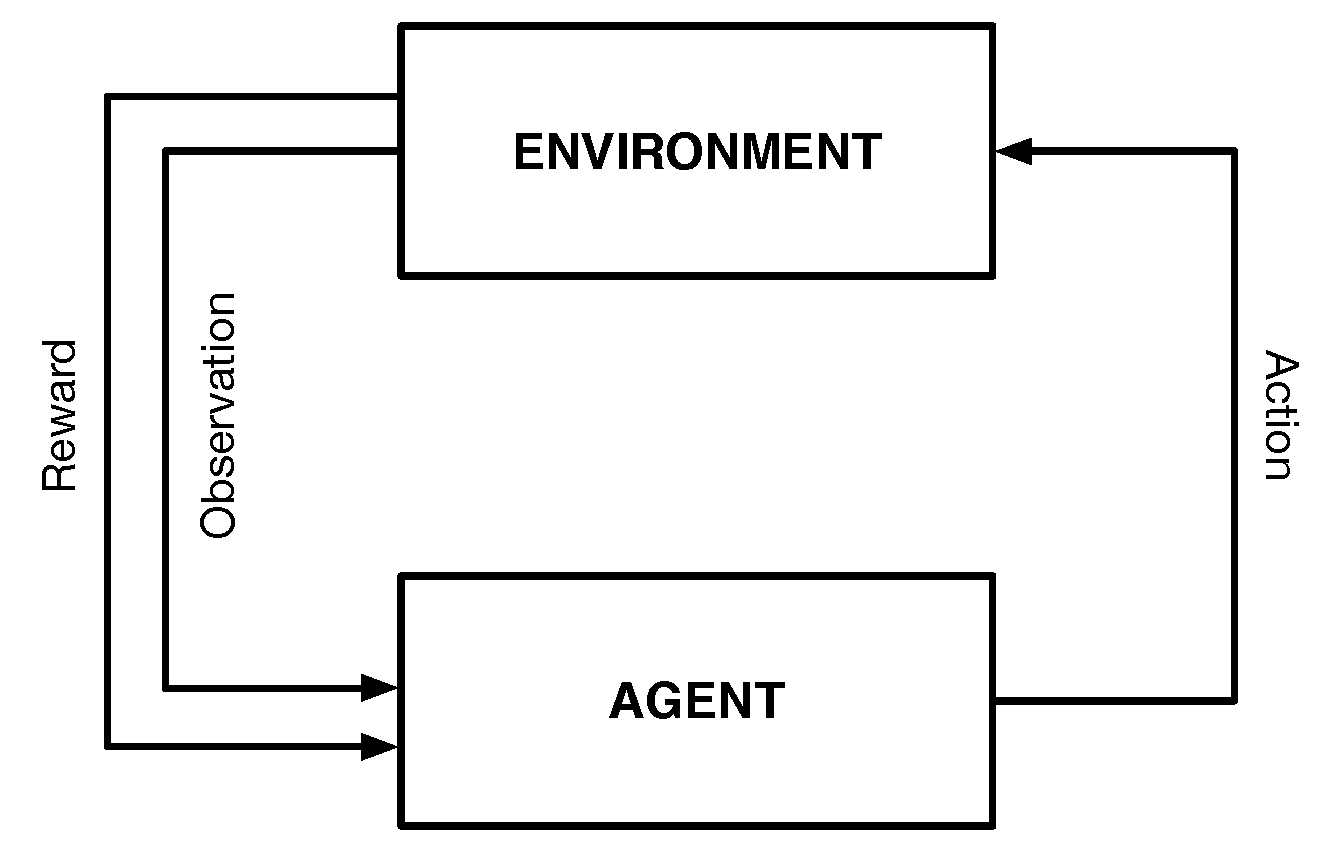
\includegraphics[width=\textwidth]{images/agent-environment.pdf}
\caption{The reinforcement learning process}
\label{fig:agentandenvironment}
\end{figure}
After the action is taken, the state of the environment changes and the agent then receives a new observation of it, and then the process repeats.  The goal of the reinforcement learning agent is to maximize the reward received over a certain time period, finding a balance between immediate and future rewards. 
\end{comment}

Reinforcement learning is an approach to the learning from experience problem in artificial intelligence. A reinforcement learning algorithm's intelligence is built upon having experiences which are then incorporated into the algorithm's own domain knowledge. This knowledge is then used to make intelligent decisions in the future \parencite{barto1998reinforcement}.

\begin{figure}[H]
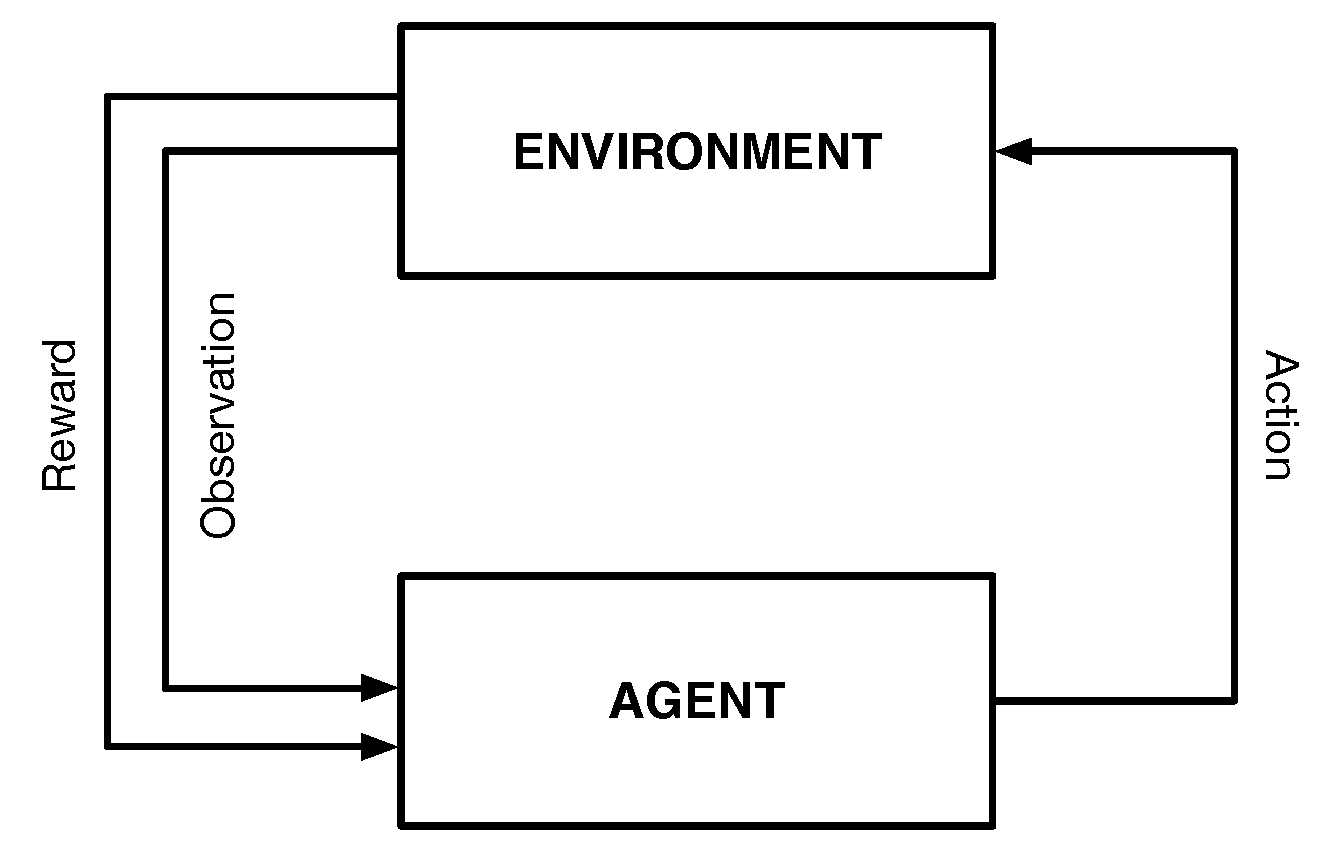
\includegraphics[width=\textwidth]{images/agent-environment.pdf}
\caption{The reinforcement learning process}
\label{fig:agentandenvironment}
\end{figure}

The reinforcement learning problem is modeled as a sequential decision problem, see figure \ref{fig:agentandenvironment} for a graphical representation of the process. A learning algorithm, an agent, performs an action and receives a reward according to some measure of how desirable the results of the action are.  After the action is taken, the state of the environment changes and the agent then receives a new observation of it, and then the process repeats. The goal of the reinforcement learning agent is to maximize the reward received over a certain time period, finding a balance between immediate and future rewards \parencite{barto1998reinforcement}. 


%One thing that sets reinforcement learning apart from other fields within artificial intelligence is that a reinforcement learning problem is solved by an online algorithm. That is, a reinforcement learning algorithm learns about its task and environment while operating in the environment. The actions taken by the agent affect what it knows about the environment, and thus its appraisal of the value of future actions and/or states of the environment.


There are several ways of further dividing reinforcement learning problems into other subcategories. Some examples are the dichotomies 1) episodic/non-episodic problems 2) problems with continuous/discrete state spaces 3) problems with continuous/discrete action spaces 4) problems with one/multiple concurrent agents. (etc.) In the text below, the two first of these dichotomies, which are relevant to this thesis, are discussed. 

\subsection{Episodic and Non-episodic Problems}
One can categorize reinforcement learning problems based on whether or not the time steps are divided into episodes. When the time steps for the agent-environment interaction are divided into subsequences in this manner, the problem is called episodic. This is common in for example games, which end when they are won or lost. If the problem is not episodic, it is called non-episodic, which means, consequently, that the interaction is not divided into subsequences. Instead, the interaction between the actor and environment goes on continually without end \parencite{barto1998reinforcement}. Two examples of non-episodic applications are controlling a robot arm (as well as other robotics problems) and maneuvering a helicopter \parencite{ng2006autonomous}. 

\subsection{Continuous and Discrete Problems}
An alternative way to categorize reinforcement learning problems is based on whether their state spaces are continuous or discrete. An important difference between the two kinds of problems is how an agent can treat similar states in the model. In a continuous problem it is a lot easier to group together states located around the same ``position'' due to the nature of a continuous problem, where the states usually more or less meld together. For example, if the reinforcement learning problem is to control a robot arm whose position is the state of the environment, the different states located around the same general area are not very different. This means that they might be treated in the same way or a similar way by an agent. On the other hand, consider the discrete problem of a game of connect four, wherein the placement of a coin into one of two adjacent slots could dramatically change the evaluation of the state and the outcome of the game \parencite{barto1998reinforcement}.

psection{Markov decision process}

Within reinforcement learning, the concept of Markov secision processes (MDP) is central. An MDP is a way to model an environment where state changes in it are dependent on both random chance and the actions of an agent. An MDP is defined by the quadruple $\left( S, A, P( \cdot , \cdot, \cdot ) , R( \cdot , \cdot ) \right)$ \parencite{altman2002applications}: 

\begin{description}
\item[$S$] \hfill \\ 
    A set of states representing the environment.
\item[$A$] \hfill \\ 
    A set of actions that can be taken.
\item[$P \colon S \times A \times S \to \mathbb R$] \hfill \\ 
    A probability distribution over the transitions in the environment. This function describes the probability of ending up in a certain target state when a certain action is taken from a certain origin state. 
\item[$R \colon S \times A \to \mathbb{R}$] \hfill \\ 
    A function for the reward associated with a state transition. In some formulation of MDPs the reward function only depends on the state.
\end{description}

MDPs are similar to Markov chains, but there are two differences. First, there is a concept of rewards in MDPs, which is absent in Markov chains. Second, in a Markov chain, the only thing that affects the probabilities of transitioning to other states is the current state, whereas in an MPD both the current state and the action taken in that state are needed to know the probability distribution connected with the next state \parencite{altman2002applications}.


\input{Technical_Background/MDP/markov_property.tex}
\input{Technical_Background/MDP/sparse_mdps.tex}
\input{Technical_Background/MDP/factored_representations.tex}


\section{Basic algorithms for solving MDPs}

A policy $\pi$ is a function from a state $s$ to an action $a$ that operates in
the context of a Markov Decision Process, i.e. $\pi \colon S \to A$. A policy
is thus a description of how to act in each state of an MDP. An arbitrary
policy is denoted by $\pi$ and the optimal policy (the policy with the largest
expected reward in the MDP) is denoted by $*$. The rest of this section is
describes some basic algorithms for solving, that is to say finding an optimal
policy, in an MDP.

\subsection{Value functions}

To solve an MDP most algorithms uses an estimation of values of states or
actions. Two value functions are usually defined, the state-value function $V :
S \to \mathbb R$ and the state-action-value function $Q : S \times A \to
\mathbb R$. As the names implies $V$ signifies how good a state is, while $Q$
signifies how good an action in a state is. The state-value function,
$V^\pi(s)$, returns the expected value when starting in state $s$ and following
policy $\pi$ thereafter. Equations \eqref{equation:v_finite} and \eqref{equation:v_infinite} show the equations for the state-value function for a finite time horizon and an infinite, discounted, time horizon respectively. In \eqref{equation:v_infinite}, $\gamma$ is the discount factor, a value between 0 and 1 which describes how fast the value of expected future rewards decay as one looks further into the future. The state-action-value function $Q^\pi(s, a)$ returns
the expected value when starting in state $s$ and taking action $a$ and
thereafter following policy $\pi$. The value functions for the optimal policy
are denoted by $V^*(s)$ and $Q^*(s, a)$. Formulas for the state-action value functions are anologous to those presented for the state value functions. 

\begin{align}
\label{equation:v_finite}
V_t^\pi(s) = \mathbb{E} \{ \sum_{k=0}^{T=k} r_{t+k} | S_t = S, \pi \}
\end{align}

\begin{align}
\label{equation:v_infinite}
V_{0}^\pi(s) = \mathbb{E} \{ \sum_{t=0}^\infty r_{t}\gamma^t | S_0 = S,\pi \}
\end{align}

Both $V^\pi$ and $Q^\pi$ can be estimated from experience. This can be done by
maintaining the average of the rewards that have followed each state when
following the policy $\pi$. When the number of times the state has been
encountered goes to infinity, the average over these histories of rewards
converges to the true values of the value function
\parencite{barto1998reinforcement}.

\input{Technical_Background/ValueFunctions/dynamic_programming.tex}
\input{Technical_Background/ValueFunctions/policy_iteration.tex}
\input{Technical_Background/ValueFunctions/value_iteration.tex}


\subsection{\etre\ in Factored Markov Decision Processes 
\note{N}}
\label{sec:e3_factored_discussion}

\paragraph{General shape of the results} In a comparison of the \etre\ agent's behavior in the different-size environments, the similarity of the shape of the graphs is striking. At first there is a period of lower and lower performance. (For the smallest environments, this period is very short, however.) Next, there is a period of fairly constant high performance, which lasts until the end of the experiment.  

This shape can be explained as a consequence of the different phases of operation of the \etre\ algorithm coupled with the structure of the MDP studied. In the beginning of the experiment, the algorithm will spend almost all of its time in the balanced wandering and exploration phases. The longer the agent has been exploring, and the more states become known, the further the agent has to explore into hard-to-reach parts of the MDP to find unexplored states. Now, in the case of the invasive species environment with the parameters chosen as in the experiments presented, the most easily reachable states are the ones where there is no tamarisk infection. This means that the harder a state is to reach, the more infected it will be, and thus the performance of the \etre\ agent in the exploration phase will fall as the experiment progresses. 

However, once the agent knows enough about the environment to enter the exploitation phase, the \etre\ agent spends close to no time at all exploring unknown states, and it retains high performance. 

\paragraph{Consequences of pooling observation data} An interesting result is that the agent is able to enter the exploitation phase for the 10 reaches/1 habitat per reach test setup slightly earlier than for the 5 reaches/1 habitat per reach setup. This is probably connected to the optimization described in the last paragraph of section \ref{sec:factored_e3}. In the 10 reaches/1 habitat per reach case there are nine reaches with two parents (including the reach itself) and one reach with only itself as parent. In the 5 reaches/1 habitat per reach case there are four reaches with two parents and one reach with only itself as parent. Since observations for state variables with similar parent structure are pooled by our \etre\ implementation, the agent will receive almost double the information per time step for the two-parent reaches in the 10 reaches case as compared to the 5 reaches case.  

\paragraph{Possible issues with the one-policy-per-reach optimization} In section \ref{sec:one_policy_per_state_variable} an optimization is described that works very well for the particular environment and environment settings that the agent was tested for. However, this optimization makes several assumptions that may cause problems if the settings are changed. For instance, one assumption is that the state of a reach is only affected directly by its adjacent parents in the DBN. If the state of a reach was made to depend significantly on other reaches two or more levels up in the river network, the agent would probably not be able to converge on an optimal policy. 

Another assumption that could lead to problems with other environment settings is the assumption that the maximal action cost in the environment is impossible or very hard to break. The invasive species environment has a maximum cost for actions. However, with the standard settings it is mathematically impossible to break this maximum. Our implementation of \etre\ would achieve very poor performance if this was not the case, since a large penalty is given when the maximum action cost is breached. 

\paragraph{DBN structure} Finally, in the invasive species environment, the structure of the DBN underlying the MDP is known at the start of the experiment, so the agent does not need to infer it from its observations. If this was not the case, all the DBN optimizations would be useless unless some kind of algorithm for infering the DBN structure was added to the agent. 

\chapter{Environment and algorithms}
\label{ch:algo}

This chapter gives a description of the environment and the algorithms that
were used in the experiment described in chapter \ref{ch:method}. The environment Invasive Species, is a simulation of a river network with invading species where to goal is to eradicate unwanted species and is further described in section \ref{sec:experiment_env}. 

Two algorithms are covered in this chapter, both of which deal with the
problems that arise with large state spaces; however, they differ in the
methods they apply. In the following chapter the general ideas behind the
algorithms, as well as specific details, are presented. 

The model-based interval estimation algorithm, described in
section~\ref{sec:mbie}, utilizes clever estimations of confidence intervals for
the Q-value functions to improve performance in sparse MDPs.
Section~\ref{sec:fac_e3} is on an algorithm that uses dynamic bayesian networks
and factored representations to improve the \etre\ algorithm to efficiently
deal with factored MDPs. 

\section{Environment specification, Invasive Species}
\label{sec:experiment_env}

When the agents were tested, the Invasive Species environment from the 2014 edition of
the Reinforcement Learning Competition was used. The environment is a
simulation of an invasive species problem, in this case a river network with
invading species where the goal of the agent is to eradicate unwanted species
while replanting native species. 

The environment's model of the river network has parameters, such as the size
of the river network and the rate at which plants spread, which can be
configured in order to create different variations of the environment.  The
size of the river network is defined by two parameters: the number of reaches
and the number of habitats per reach. A habitat is the smallest unit of land
that is considered in the problem. A habitat can either be invaded by the
tamarix, which is an unwanted species, empty or occupied by native species. A
reach is a collection of neighboring habitats. The structure of the river
network is defined in terms of which reach is connected to which
\parencite{invasiveSpecis2014:Online}. In figure \ref{fig:river} a model of a
river network is shown.

\begin{figure}[ht]
\centering
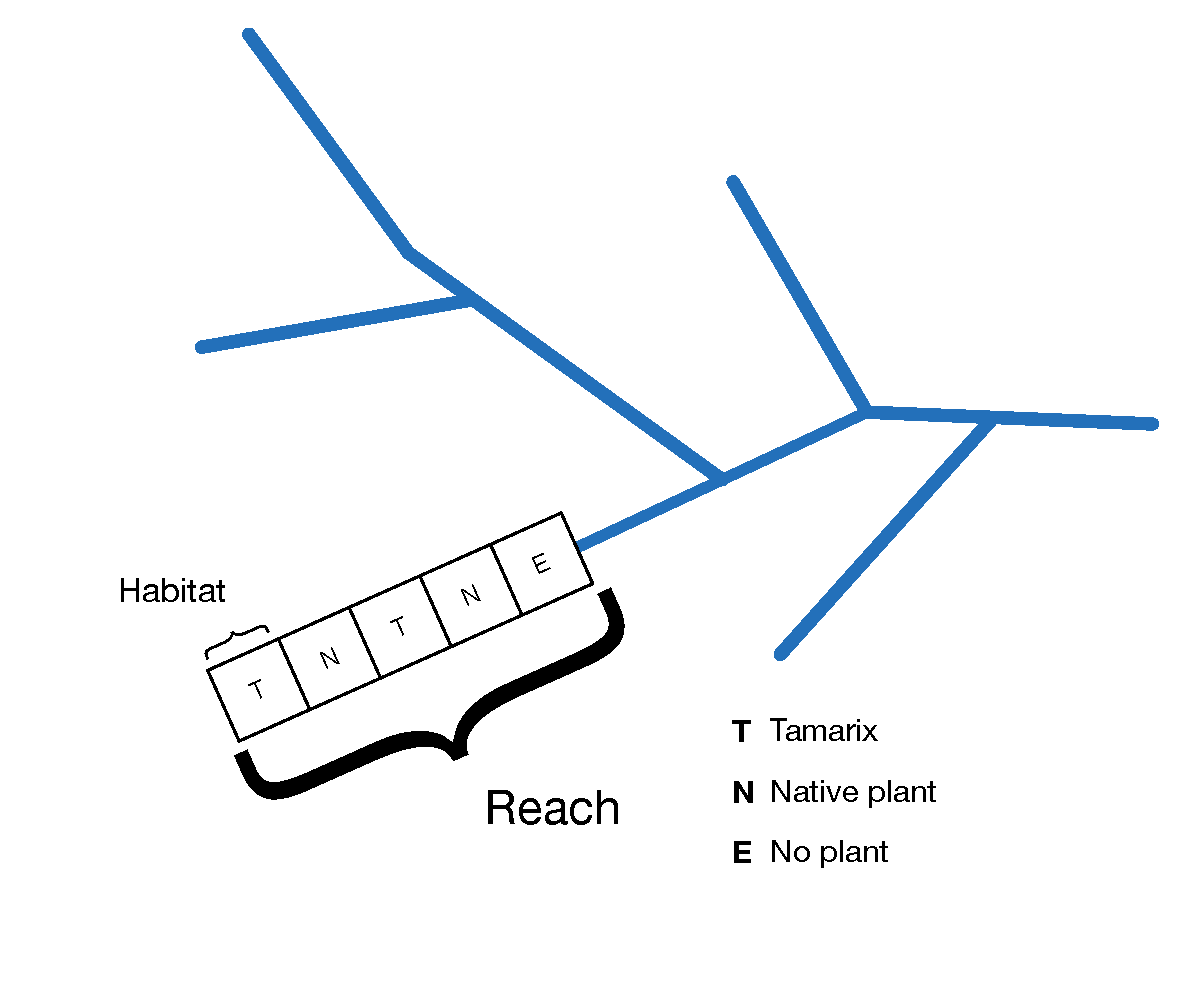
\includegraphics[width=0.9\textwidth]{images/river_network.pdf}
\caption{A river network, as modeled by the Invasive Species reinforcement learning environment.}
\label{fig:river}
\end{figure}

There are four possible actions (eradicate tamarix trees, plant native trees,
eradicate tamarix trees and plant native trees and a wait-and-see action),
and the agent chooses one of these actions for each reach and time step. If the 
agent chooses to eradicate tamarix trees or plant native trees in a reach, 
all habitats of that reach are targeted by this action. What
actions are available to the agent depends on the state of each reach. It is
always possible to choose the wait-and-see action, but there has to be one
or more tamarix-invaded habitats in a reach for the eradicate or eradicate and
plant actions to be available and there has to be at least one empty habitat in
a reach for the plant-native-trees action to be available
\parencite{invasiveSpecis2014:Online}.  

\section{Model-based interval estimation}
\label{sec:mbie}

Model-based interval estimation is a modification of value iteration whose main feature is its  addition of confidence
intervals to the state-action values. These confidence intervals allow the agent to choose between
actions, based on how confident it is about its evaluation of them. In effect,
the less certain the agent is about its evaluation of the states and actions,
the more exploratory the actions will be. When the agent is more confident
however, it will exploit what it has learnt so far about the MDP
\parencite{dietterich2013pac}.

\input{algorithms/MBIE/modification_of_value_it}
\input{algorithms/MBIE/gt.tex}
\input{algorithms/MBIE/modded_bounds}

\section{\etre\ in factored Markov decision processes}
\label{sec:fac_e3}

The second algorithm studied in this thesis is a version of the \etre\ algorithm that focuses on factored problem domains by modeling them as a dynamic Bayesian network. The original \etre\ algorithm is described in section \ref{sec:e3}, which gives a broad overview along with the key strategies used in the algorithm. The following section, \ref{sec:factored_e3}, considers some ways to extend the original algorithm and make use of factored representations and planning in factored domains to improve the running time of the algorithm.

\input{algorithms/Factored_E3/e3.tex}
\input{algorithms/Factored_E3/factored_additions.tex}


\chapter{Method}
\label{sec:method_intro}

This chapter covers the preliminaries and preparations carried out before the
execution of the experiments. It covers  and how the agents described in chapter
\ref{ch:algo} were implemented and the additions and modifications that were made to them. The chapter
concludes with a description of the tools used for the experiment.
\section{Algorithm implementation}
\label{sec:implementation}

We implemented two existing algorithms and we also added some extensions.  The
experiment utilized RL-Glue (section~\ref{sec:rl_glue}) to connect the agents
and environment to each other.  To verify the behavior of our agents we utilized smaller
environments (see sections~\ref{sec:intro_grid_world} and \ref{sec:ns}) where
the correct operation is either easy to derive or obvious from inspection. By
starting with smaller problems and using an iterative approach it was possible
to identify bottlenecks in our implementations and correct possible errors
early.

\input{algorithms/MBIE/modded_bounds}

\input{method/ConstructingExperiments/contributionse3}

\subsection{GridWorld}
\label{sec:intro_grid_world}

The GridWorld environment was implemented to easily be able to verify the
correctness of the MBIE algorithm. It consists of a grid of twelve squares with
one blocked square, one starting square, one winning square, one losing square and
eight empty squares. The agent can take five actions, north, south, west,
east or exit. The exit-action is only possible from the winning or losing
state. When taking an action being in one state and the action is directed to
another empty state there is an 80\% probability to succeed and 10\%
probability to fail and 10\% to go sideways.

\subsection{Network simulator}
\label{sec:ns}

A simple computer network simulation was implemented to verify the behavior of an
early version of \etre\ algorithm. In this environment, the agent tries to keep
a network of computers up and running. All computers start in the running
state, but there is a chance that they randomly stop working. If a computer is
down, it has a chance to cause other computers connected to it to also fail. In
each time step, the agent chooses one computer to restart, which with 100
percent probability will be in working condition in the next time step. The
agent is rewarded for each computer in the running state after each time step. 

\section{Our contributions}
\label{sec:contributions}


\input{algorithms/MBIE/modded_bounds}


\input{method/ConstructingExperiments/contributionse3}

\section{Environment specification}
\label{sec:experiment_env}

For the experiment, the Invasive Species environment from the 2014 edition of
the Reinforcement Learning Competition was used. The environment is a
simulation of an invasive species problem, in this case a river network with
invading species where the goal of the agent is to eradicate unwanted species
while replanting native species. 

The environment's model of the river network has parameters, such as the size
of the river network and the rate at which plants spread, which can be
configured in order to create different variations of the environment.  The
size of the river network is defined by two parameters: the number of reaches
and the number of habitats per reach. A habitat is the smallest unit of land
that is considered in the problem. A habitat can either be invaded by the
tamarix, which is an unwanted species, empty or occupied by native species. A
reach is a collection of neighboring habitats. The structure of the river
network is defined in terms of which reach is connected to which
\parencite{invasiveSpecis2014:Online}. In figure \ref{fig:river} a model of a
river network is shown.

\begin{figure}[ht]
\centering
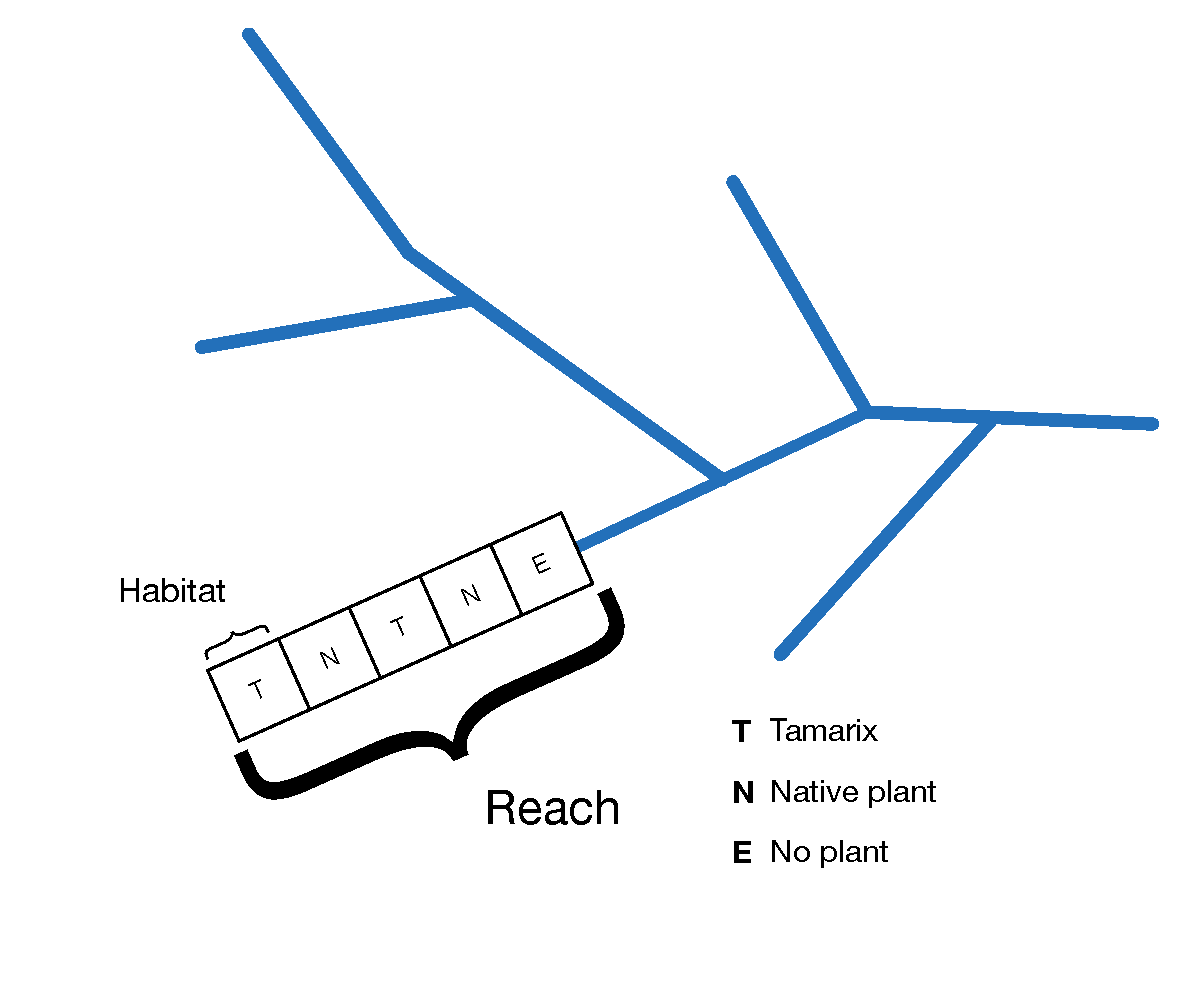
\includegraphics[width=0.9\textwidth]{images/river_network.pdf}
\caption{A river network, as modelled by the Invasive Species reinforcement learning environment.}
\label{fig:river}
\end{figure}

There are four possible actions (eradicate tamarisks, plant native trees,
eradicate tamarisks and plant native trees, and finally a wait-and-see action),
and the agent chooses one of these actions per reach per time step. What
actions are available to the agent depends on the state of each reach. It is
always possible to choose the wait-and-see action, but there has to be one
or more tamarix-invaded habitats in a reach for the eradicate or eradicate and
plant actions to be available and there has to be at least one empty habitat in
a reach for the plant-native-trees action to be avalable
\parencite{invasiveSpecis2014:Online}. 

\section{Test specification}
\label{sec:test_spec}

The testing of the agents required us to choose certain sets of parameters, for
the environment, the two different agents and the experiment itself. 

\paragraph{Environment parameters}

The Invasive Species environment requires a number of parameters. For further
explanation of the environment parameters consult the environment
webpage\footnote{\url{http://2013.rl-competition.org/domains/invasive-species}}.
The specific parameters used are presented in
appendix~\ref{ap:environment_spec}.

\paragraph{Agent Parameters}

The agents evaluated required different types of parameters. Some preliminary
tests were run and then the parameters giving best results were chosen.
Parameters for MBIE are found in table~\ref{tab:mbie_params_both}.

\begin{table}[H]
\centering
\captionof{table}{Parameters for MBIE}
\label{tab:mbie_params_both}

\begin{subfigure}[b]{0.47\textwidth}
    \centering
    \captionof{table}{Proper MBIE}
    \label{tab:mbie_params} 
    \begin{tabular}{lr}
     \toprule
     Parameter & Value \\
     \midrule
     Discount factor, $\gamma$ & 0.9 \\
     Confidence, $\delta$ & 95\% \\
     $\Delta \omega$ & $\frac{1}{2}\sqrt{\frac{2|ln(2^{|S|}-2) - ln  \delta |}{N(s,a)}}$ \\
     
     \bottomrule
    \end{tabular}
\end{subfigure}
\quad
\begin{subfigure}[b]{0.47\textwidth}
    \centering
    \captionof{table}{Realistic MBIE}
    \label{tab:mbie_realistic_params}
    \begin{tabular}{lr}
     \toprule
     Parameter & Value \\
     \midrule
     Discount factor, $\gamma$ & 0.9 \\
     $\Delta \omega$ & $1 - 0.05 N(s,a)$ \\
     \bottomrule
    \end{tabular}
\end{subfigure}
\end{table}

For DBN-\etre\ a higher exploration limit resulted in the agent starting to
exploit earlier but with a slightly lower final return. A higher partial state
known limit resulted in later exploitation but no appreciable difference in
final return. The values in table~\ref{tab:dbne3_params} were a good middle
ground.

\begin{table}[H]
\captionof{table}{DBN-\etre\ parameters}
\label{tab:dbne3_params}
\centering
\begin{tabular}{lr}
 \toprule
 Parameter & Value \\
 \midrule
 Discount factor & 0.9 \\
 Exploration limit & 5\% \\
 Partial state known limit & 5 \\
 \bottomrule
\end{tabular}
\end{table}

\paragraph{Experiment parameters}

The tests performed had to be long enough to sample enough data to extract
relevant results without making the running time too long. A single test
consisted of a specific number of episodes with a specific length. A good
combination was required to efficiently evaluate the agents. If a single
episode consisted of too many samples it would be difficult to see the learning
process as results are reported as total reward over an episode and that
process might be hidden as its impact on the total reward is smaller with a
longer episode. On the other hand, if an episode length is too short it would
end before the agents could do any valuable learning.

In addition to a satisfactory episode length, a reasonable number of episodes
needs to be sampled for it to be possible to draw conclusions from the results.
If the number of episodes is too small, the convergence of the agents cannot be
seen. However, if the number of episodes are too large a lot of sampled data
would be redundant for the study. Some preliminary experiments were run in
order to tune the experiment parameters to suitable values. The episode length
was set to 100 samples and there were 100 episodes per test.

To evaluate the agents in the Invasive Species environment combinations of
reaches and number of habitats per reach that can be seen in
table~\ref{tab:reaches_habitats} were choosen. Combinations were chosen to have
a wide range in the total number of states for the agents to deal with and to
test how the agents deal with taking actions that have to take into account
several state components. 

As seen in table ~\ref{tab:reaches_habitats}, the state count increases rapidly
when habitats are added to the problem. This is obvious from the fact that the state count
depends exponentially on the total number of habitats; see equation \eqref{eq:statecount}, where $h$ is the number of habitats per reach and $r$ is the number of reaches.

\begin{equation}
\label{eq:statecount}
 |S| = 3 ^ {hr}
\end{equation}

\begin{table}[H]
\centering
\caption{Combinations of reaches and habitats used in testing.}
\label{tab:reaches_habitats}
\begin{tabular}{rrr}
 \toprule
 Reaches & Habitats per reach & Total state count \\
 \midrule
 5  & 1 &          243 \\
 3  & 2 &          729 \\
 3  & 3 &      19\,683 \\
 10 & 1 &      59\,049 \\
 4  & 3 &     531\,441 \\
 5  & 3 & 14\,348\,907 \\
 \bottomrule
\end{tabular}
\end{table}

\section{Programming environment}
\label{sec:prog_env}

The Java programming language 1.7 was used to implement the algorithms. In addition, the
Java version of RL-Glue framework version 3.0 was used. For version control Git
was used, due to its simplicity and performance.

\section{RL-Glue}
\label{sec:rl_glue}

To evaluate the agents the RL-Glue framework was used, which acts as an
interface for communication between the agent and the environment. The software
uses the RL-Glue protocol, which specifies how a reinforcement learning problem
should be divided when constructing experiments and how the different programs
should communicate \parencite{tanner2009rl}.

RL-Glue divides the reinforcement learning process into three separate
programs: an agent, an environment and an experiment. RL-Glue provides a server
software that manages the communication between these programs. The agent and
the environment programs are responsible for executing the tasks as specified
by RL-Glue and the experiment program acts as a bridge between the agent and
environment \parencite{tanner2009rl}.

The modular structure of RL-Glue makes it easier to construct repeatable
reinforcement learning experiments. By separating the agent from the
environment it is possible to reuse the environment and switch out the agent.
It also makes it a lot easier to cooperate and continue working on existing
environments implemented by other programmers.


\chapter{Result}

\newcommand{\graphwidth}{0.70\textwidth}
\newcommand{\testsubfigure}[2]{%
\begin{subfigure}[b]{\graphwidth}
    \includegraphics[width=1.1\textwidth]{images/tests/#1r-#2h.pdf}
    \caption{#1 reaches and #2 habitats per reach}
    \label{fig:#1r#2h}
\end{subfigure}
}

In figures~\ref{fig:tests1}, \ref{fig:tests2} and \ref{fig:tests3} we have test results from running our agents on the invasive species environment on different sizes of river network. The raw data can be found in appendix~\ref{ap:result_tables}.

\begin{figure}[h!]
    \centerline{
    \testsubfigure{3}{3}
    ~
    \testsubfigure{3}{2}
    }
    \caption{Test runs with different number of reaches and habitats}
    \label{fig:tests1}
\end{figure}

\begin{figure}[h!]
    \centerline{
    \testsubfigure{5}{1}
    ~
    \testsubfigure{5}{3}
    }
    \caption{Test runs with different number of reaches and habitats}
    \label{fig:tests2}
\end{figure}

\begin{figure}[h!]
    \centerline{
    \testsubfigure{4}{3}
    ~
    \testsubfigure{10}{1}
    }
    \caption{Test runs with different number of reaches and habitats}
    \label{fig:tests3}
\end{figure}

The agent learns for 100 episodes with 100 samples per episode, other parameters are specified in section~\ref{sec:test_spec}. The invasive species environment associates a certain cost with each state and action, thus the reward is always negative. In each test the reward varies over time for the MBIE agent, the realistic MBIE agent and the DBN-\etre\ agent.

With smaller state spaces (see figure~\ref{fig:3r3h}, \ref{fig:3r2h} and \ref{fig:5r1h}) we can see that the realistic MBIE agent outperforms the proper MBIE agent and comes close to the DBN-\etre\ agent. In the tests where the state space is larger (see figure~\ref{fig:5r3h}, \ref{fig:10r1h} and \ref{fig:4r3h}) proper MBIE and realistic MBIE are very close to each other in performance while the DBN-\etre\ agent outperforms both. The realistic MBIE algorithm performs better in with smaller state spaces due to more states becoming known quicker and thus having their true value.

In each of the test runs the DBN-\etre\ algorithm exhibits a period of learning that corresponds to exploration (as described in section~\ref{sec:e3}) where the agent has not explored the environment enough and seeks more information. This is apparent in figure~\ref{fig:3r3h}.
\chapter{Discussion \note{B}}
\label{ch:discussion}
This chapter is a discussion of the results and method used in the project. The algorithms are evaluated with regard to their performance achieved in the tests, which is used as a basis when comparing them against each-other. Determining their strengths and weaknesses and if they were suitable for problems with an environment that has a large discrete state space and in particular for the environment Invasive Species. There is also a discussion on ethical aspects regarding the work in this thesis.


% Det behövs inte en ingående disposition här, det tar ner läsligheten. Det som tas upp i styckena är vettigt, men detta är inte rätt ställe för dem.

% This chapter is a combination of discussion of the results of using the algorithms described in chapter \ref{ch:algo}, together with a examination of the method used in the project. The algorithms is evaluated with regard to their performance achieved in the experiments \ref{sec:constructing_experiments}, which is used for a basis when comparing them against each-other. Focusing on their strengths and weaknesses and circling around the question why did they perform as they did. Were they suitable for this kind of problem, an environment with a large discrete state space and in particular for this thesis a simulation of an Invasive Species environment.

% The second part of this chapter contains a section containing a presentation of similar studies conducted, summarizing their results and opinions. Using their finding as a basis, there will also be a discussion regarding its connection to the results in this thesis. With inspiration from similar studies in combination with the results of this thesis, a discussion about the possible extensions and additional work or unanswered questions in this thesis are presented. 

%In order to round of this chapter, the last section of this chapter revolves around ethical questions and aspects regarding the theme of this topic. The main theme of the last section is ethical aspects in \acrlong{ai} \acrshort{ai}, \acrfull{ai}, along with a discussion about the usefulness of Reinforcement Learning in today's society with focus on using simulations.

\section{Evaluation of the agents \note{I}}
\label{sec:coa}

\input{Discussion/AlgorithmsEvaluation/dbn.tex}
\input{Discussion/AlgorithmsEvaluation/mbie.tex}
\input{Discussion/AlgorithmsEvaluation/discussion_diffrences}




\section{Potential factors impacting the results}
\label{sec:truth_results}

There are several factors that possibly reduce the reliability of the results. For instance, all evaluations used only one environment, the implementation of the algorithms could contain errors and the correct results for all test runs are not always known. 

\input{Discussion/discussion_results/impact_of_one_env.tex}

\input{Discussion/discussion_results/implementation_of_algorithms.tex}

\input{Discussion/discussion_results/testing_methodology.tex}


%\section{Similar Studies \note{N, K}}
The work with reducing the complexity of the reinforcement learning problems with environments containing large state spaces is not a new research topic. However, this thesis is taking a rather uncommon approach to the problem. Instead of trying to derive new algorithms for solving the problem, the focus is instead focused on usefulness of research conducted within the area of reinforcement learning problems. To be even more specific this thesis has zoomed in on two possible attempts on solving the problem with environments containing large state spaces. An approach that is rather uncommon and thus similar studies is as well uncommon. 
%Behöver skrivas om, tydligare
Thereby this section will combining focus on both studies similar to this thesis comparing the usefulness of research already conducted along with a summarized study of studies of work being done to reduce the complexity of environments with large state spaces.

\todo[inline]{Samma miljö kanske, dess pac?}

\paragraph{Similar Studies Regarding Comparing Existing Research}
\todo[inline]{Borde finnas återkoppling i diskussion kring detta}
It has been shown in Strehl and Littman (2004; 2008) that MBIE outperforms \etre\ in the MDPs RiverSwim and SixArms. \parencite{dietterich2013pac}


\paragraph{Large State Spaces using Dynamic Bayesian Networks}
This paragraph is devoted to similar methods using dynamic Bayesian networks as an underlying representation in order to model the structure of the environment. Due to the relevance of using dynamic Bayesian network as a method for tackling similar problems it is thesis on its own in order to summarize them all. It is also possible to study section \ref{sec:better_planing_algos} for further references, however their main focus on the planning algorithm.

An algorithm to DBN-\etre\ is the algorithm by \textcite{ross2012model} which is as well utilizing a factored representation for the underlying structure. However, in the DBN-\etre\ algorithm no planning algorithm was specified and therefore leaving an empty square in the implementation affecting the overall complexity of the algorithm. In the algorithm by \textcite{ross2012model} 

\todo[inline]{Resultatjämförelse}

\paragraph{Similar Studies Regarding Large State Spaces Using Model Based Something grejen}
Grattis MBIE, er punkt.

\section{Ethical and social aspects of artificial intelligence}

\input{Discussion/Ethics/intro.tex}

\input{Discussion/Ethics/invasive_species.tex}

\input{Discussion/Ethics/ai_right_or_wrong.tex}



\section{Further work}

In this section we discuss possible further work and extensions to our thesis.

\input{Discussion/further_work/more_test_envs.tex}
\input{Discussion/further_work/better_planning_dbn.tex}
\input{Discussion/further_work/MBIE.tex}
\input{Discussion/further_work/mbie_should_use_dbn.tex}


\printbibliography

\begin{appendices}

\chapter{Environment specification}
\label{sec:environment_spec}

\begin{table}[H]
\centering
\captionof{table}{Dynamic parameters common to both species}
\label{tab:dynamic_params_common} 
\begin{tabular}{l r}
 \toprule
 Parameter & Value \\
 \midrule
 Eradication rate & 0.85 \\
 Restoration rate & 0.65 \\
 Downstream spread rate & 0.5 \\
 Upstream spread rate & 0.1 \\
 \bottomrule
\end{tabular}
\end{table}

\begin{table}[H]
\centering
\captionof{table}{Dynamic parameters different between the species} \label{tab:dynamic_params_not_common}
\begin{tabular}{lrr}
\toprule
 Parameter & Native & Tamarisk \\
 \midrule
 Death rate & 0.2 & 0.2 \\
 Production rate & 200 & 200 \\
 Exogenous arrival\footnote{Arrival of seeds from outside the environment} & Yes & Yes \\
 Exogenous arrival probability & 0.1 & 0.1 \\
 Exogenous arrival number & 150 & 150 \\
 \bottomrule
\end{tabular}
\end{table}

\begin{table}[H]
\centering
\captionof{table}{Cost function parameters} \label{tab:cost_params} 
\begin{tabular}{lr}
 \toprule
 Parameter & Value \\
 \midrule
 Cost per invaded reach & 10 \\
 Cost per tree & 0.1 \\
 Cost per empty slot & 0.01 \\
 Eradication cost & 0.5 \\
 Restoration cost & 0.9 \\
 \bottomrule
\end{tabular}
\end{table}

\begin{table}[H]
\centering
 \captionof{table}{Variable costs depending on number of habitats affected by action}
 \begin{tabular}{lr}
 \toprule
 Parameter & Value \\
 \midrule
 Eradication cost & 0.4 \\
 Restoration cost for empty slot & 0.4 \\
 Restoration cost for invaded slot & 0.8 \\
 \bottomrule
\end{tabular}
\label{tab:cost_params_var}
\end{table}
\end{appendices}


\end{document}

\chapter{Result}

\newcommand{\graphwidth}{0.70\textwidth}
\newcommand{\testsubfigure}[2]{%
\begin{subfigure}[b]{\graphwidth}
    \includegraphics[width=1.1\textwidth]{images/tests/#1r-#2h.pdf}
    \caption{#1 reaches and #2 habitats per reach}
    \label{fig:#1r#2h}
\end{subfigure}
}

In figures~\ref{fig:tests1}, \ref{fig:tests2} and \ref{fig:tests3} we have test results from running our agents on the invasive species environment on different sizes of river network. The raw data can be found in appendix~\ref{ap:result_tables}.

\begin{figure}[h!]
    \centerline{
    \testsubfigure{3}{3}
    ~
    \testsubfigure{3}{2}
    }
    \caption{Test runs with different number of reaches and habitats}
    \label{fig:tests1}
\end{figure}

\begin{figure}[h!]
    \centerline{
    \testsubfigure{5}{1}
    ~
    \testsubfigure{5}{3}
    }
    \caption{Test runs with different number of reaches and habitats}
    \label{fig:tests2}
\end{figure}

\begin{figure}[h!]
    \centerline{
    \testsubfigure{4}{3}
    ~
    \testsubfigure{10}{1}
    }
    \caption{Test runs with different number of reaches and habitats}
    \label{fig:tests3}
\end{figure}

The agent learns for 100 episodes with 100 samples per episode, other parameters are specified in section~\ref{sec:test_spec}. The invasive species environment associates a certain cost with each state and action, thus the reward is always negative. In each test the reward varies over time for the MBIE agent, the realistic MBIE agent and the DBN-\etre\ agent.

With smaller state spaces (see figure~\ref{fig:3r3h}, \ref{fig:3r2h} and \ref{fig:5r1h}) we can see that the realistic MBIE agent outperforms the proper MBIE agent and comes close to the DBN-\etre\ agent. In the tests where the state space is larger (see figure~\ref{fig:5r3h}, \ref{fig:10r1h} and \ref{fig:4r3h}) proper MBIE and realistic MBIE are very close to each other in performance while the DBN-\etre\ agent outperforms both. The realistic MBIE algorithm performs better in with smaller state spaces due to more states becoming known quicker and thus having their true value.

In each of the test runs the DBN-\etre\ algorithm exhibits a period of learning that corresponds to exploration (as described in section~\ref{sec:e3}) where the agent has not explored the environment enough and seeks more information. This is apparent in figure~\ref{fig:3r3h}.
\chapter{Discussion \note{B}}
\label{ch:discussion}
This chapter is a discussion of the results and method used in the project. The algorithms are evaluated with regard to their performance achieved in the tests, which is used as a basis when comparing them against each-other. Determining their strengths and weaknesses and if they were suitable for problems with an environment that has a large discrete state space and in particular for the environment Invasive Species. There is also a discussion on ethical aspects regarding the work in this thesis.


% Det behövs inte en ingående disposition här, det tar ner läsligheten. Det som tas upp i styckena är vettigt, men detta är inte rätt ställe för dem.

% This chapter is a combination of discussion of the results of using the algorithms described in chapter \ref{ch:algo}, together with a examination of the method used in the project. The algorithms is evaluated with regard to their performance achieved in the experiments \ref{sec:constructing_experiments}, which is used for a basis when comparing them against each-other. Focusing on their strengths and weaknesses and circling around the question why did they perform as they did. Were they suitable for this kind of problem, an environment with a large discrete state space and in particular for this thesis a simulation of an Invasive Species environment.

% The second part of this chapter contains a section containing a presentation of similar studies conducted, summarizing their results and opinions. Using their finding as a basis, there will also be a discussion regarding its connection to the results in this thesis. With inspiration from similar studies in combination with the results of this thesis, a discussion about the possible extensions and additional work or unanswered questions in this thesis are presented. 

%In order to round of this chapter, the last section of this chapter revolves around ethical questions and aspects regarding the theme of this topic. The main theme of the last section is ethical aspects in \acrlong{ai} \acrshort{ai}, \acrfull{ai}, along with a discussion about the usefulness of Reinforcement Learning in today's society with focus on using simulations.

\section{Evaluation of the agents \note{I}}
\label{sec:coa}

\subsection{\etre\ in Factored Markov Decision Processes 
\note{N}}
\label{sec:e3_factored_discussion}

\paragraph{General shape of the results} In a comparison of the \etre\ agent's behavior in the different-size environments, the similarity of the shape of the graphs is striking. At first there is a period of lower and lower performance. (For the smallest environments, this period is very short, however.) Next, there is a period of fairly constant high performance, which lasts until the end of the experiment.  

This shape can be explained as a consequence of the different phases of operation of the \etre\ algorithm coupled with the structure of the MDP studied. In the beginning of the experiment, the algorithm will spend almost all of its time in the balanced wandering and exploration phases. The longer the agent has been exploring, and the more states become known, the further the agent has to explore into hard-to-reach parts of the MDP to find unexplored states. Now, in the case of the invasive species environment with the parameters chosen as in the experiments presented, the most easily reachable states are the ones where there is no tamarisk infection. This means that the harder a state is to reach, the more infected it will be, and thus the performance of the \etre\ agent in the exploration phase will fall as the experiment progresses. 

However, once the agent knows enough about the environment to enter the exploitation phase, the \etre\ agent spends close to no time at all exploring unknown states, and it retains high performance. 

\paragraph{Consequences of pooling observation data} An interesting result is that the agent is able to enter the exploitation phase for the 10 reaches/1 habitat per reach test setup slightly earlier than for the 5 reaches/1 habitat per reach setup. This is probably connected to the optimization described in the last paragraph of section \ref{sec:factored_e3}. In the 10 reaches/1 habitat per reach case there are nine reaches with two parents (including the reach itself) and one reach with only itself as parent. In the 5 reaches/1 habitat per reach case there are four reaches with two parents and one reach with only itself as parent. Since observations for state variables with similar parent structure are pooled by our \etre\ implementation, the agent will receive almost double the information per time step for the two-parent reaches in the 10 reaches case as compared to the 5 reaches case.  

\paragraph{Possible issues with the one-policy-per-reach optimization} In section \ref{sec:one_policy_per_state_variable} an optimization is described that works very well for the particular environment and environment settings that the agent was tested for. However, this optimization makes several assumptions that may cause problems if the settings are changed. For instance, one assumption is that the state of a reach is only affected directly by its adjacent parents in the DBN. If the state of a reach was made to depend significantly on other reaches two or more levels up in the river network, the agent would probably not be able to converge on an optimal policy. 

Another assumption that could lead to problems with other environment settings is the assumption that the maximal action cost in the environment is impossible or very hard to break. The invasive species environment has a maximum cost for actions. However, with the standard settings it is mathematically impossible to break this maximum. Our implementation of \etre\ would achieve very poor performance if this was not the case, since a large penalty is given when the maximum action cost is breached. 

\paragraph{DBN structure} Finally, in the invasive species environment, the structure of the DBN underlying the MDP is known at the start of the experiment, so the agent does not need to infer it from its observations. If this was not the case, all the DBN optimizations would be useless unless some kind of algorithm for infering the DBN structure was added to the agent. 

\subsection{MBIE}
In comparison to the DBN-\etre\ performance graphs, the MBIE performance exhibits a much smoother transition from poor to good performance. This is due to the fact that MBIE does not have a clear distinction between exploration and exploitation in phases. Instead, MBIE in effect always gives state-action pairs that are relatively unexplored a bonus to their expected value in order to promote exploration.  

In the graphs for MBIE there are several ``dips'' in performance as for example in figure~\ref{fig:tests2}b. These could be explained as cases when the algorithm by chance enters previously unexplored states and spends several steps exploring this and similar/adjacent states. 

\paragraph{Realistic MBIE and original MBIE}
The realistic version of MBIE outperforms the original MBIE in every test. This is probably explained by the fact that the state that is the easiest to arrive at is the one that gives the greatest reward (see section \ref{sec:e3_factored_discussion}). Since the realistic version of MBIE considers states known and thus evaluates them  realistically rather than optimistically much sooner than the original version of MBIE, it spends much less time exploring unknown states, which are bound to give lower rewards than the more easily explored states. 

\paragraph{Impact of planning-frequency}
A factor to be considered when viewing the results is the impact of the frequency of planning. For example when looking at large state spaces in MBIE (both versions) planning is only performed when the sample size has increased by 50\%. This is quite infrequent when viewing our tests of 100 episodes of 100 samples per episode, resulting in many episodes using the same policy and making it harder to deduce improvement over time as they come in discrete intervals rather then continuously. This issue does not arise in DBN-\etre\ which does planning continuously when required.    

%utforska runt "nya" outforskade states

% Formen annorlunda än 
%jämföra realistisk/orealistisk
% - realistisk: slutar utforska tidigare, samma orsak som beskrivs tidigare (lätt att hitta mest värdefulla statet). 
% - 
\subsection{DBN-\etre\ vs MBIE \note{N}}
An expectation on both agents is that they should converge on optimal behavior
as $t$ goes to infinity. However, it is clear from the results presented in
chapter \ref{ch:results} that neither version of the MBIE agent reaches the
same level of performance as the DBN-\etre\ agent. In the smaller problem as
seen for example in figure~\ref{fig:tests1}b the diffrence is not all that
diffrent between DBN-\etre\ agent and the realistic MBIE. 

Nevertheless, it isstill clear that DBN-\etre\ is far superior in finding the converging policy.
Previous studies have been concluded as a comparisson regarding the original
\etre\ algorithm and MBIE, in \textcite{strehl2004empirical} that MBIE
outperforms \etre\ in their testing environments. The results in this thesis
utilized a heavily optimized version of the original \etre\ agent using
factored representation and the results speak for themselfs mentioned earlier
in this report. 

However, as mentioned in the last paragraph of
section \ref{sec:e3_factored_discussion} when the structure of the underlying
MDP the benefits of using a factored representations provides a big advantage
as seen in the figures in chapter \ref{ch:results}. This also increases the
responsibility on the designer of the factored representation and if done in
the wrong way it will prove to become a bottleneck instead of a performance
increase. 

test environments are not factored, name them.
a good model > a good algorithm

\paragraph{Unfair comparisons}
In one sense, the comparison between our implementations of MBIE and DBN-\etre\
are not very fair. The DBN-\etre\ implementation has been heavily optimized to
work with factored MDPs and the invasive species environment in particular,
whereas the MBIE implementation is much more generalized. The discussions
regarding the generality of the agents in furher continued in section
\ref{sec:impact_of_one_env}. 

\paragraph{Large state spaces}
When the number of states are increased it is clear that the algorithms still
work. Comparing the 4 reaches and 3 habitats per reach case seen in
figure~\ref{fig:tests3}a with the 5 reaches and 3 habitats per reach case seen
in figure~\ref{fig:tests2}b this can be seen. The algorithms do still improve
over time although taking longer time to converge, which is expected as the
state space increases in size. 

A noteable difference between the original and realistic versions of MBIE is
that the realistic version has the same level of performance as the original
MBIE in larger state spaces whereas in smaller state spaces the realistic MBIE
was clearly better than the original. Compare figure~\ref{fig:tests1}b with
figure~\ref{fig:tests2}b to see this difference. In smaller state spaces the
realistic version will know the real value of more states than the original
version, while in larger state spaces both versions will prioritise unknown
states.

The DBN-\etre\ algorithm successfully deals with large state spaces. DBN-\etre\
utilizes a factored approach in representing transition probabilities, which
allows the algorithm to learn about the environment quicker whereas a
non-factored approach would struggle to learn the transition probabilities.
This can be seen in the result where the DBN-\etre\ algorithm quickly knows
enough to start exploiting even in cases such as figure~\ref{fig:5r3h}.
Furthermore, using a factored approach to policy calculation allows quick
policy calculations making the algorithm fast to run in large state spaces.





\section{Potential factors impacting the results}
\label{sec:truth_results}

There are several factors that possibly reduce the reliability of the results. For instance, all evaluations used only one environment, the implementation of the algorithms could contain errors and the correct results for all test runs are not always known. 

\subsection{Impact of using one environment}
\label{sec:impact_of_one_env}

The results presented in this report are only collected from one environment.
Considering this, it is challenging to evaluate and verify the generality of the
algorithms. The DBN-\etre\ algorithm is specifically optimized for the Invasive Species
environment, which reduces the credibility regarding the generality of the
techniques discussed in this thesis, due to the fact that it is not possible
within the scope of this thesis to evaluate the performance of the DBN-\etre\,
without the optimizations applied. 

The generality of MBIE is more probable due to the fact it was simultaneously
tested alongside Invasive Species in a simpler environment: GridWorld
(section~\ref{sec:intro_grid_world}), thereby forcing a degree of generality during
construction of the agent.


\subsection{Implementation of algorithms}

One of the biggest challenges when constructing and evaluating algorithms is to
validate the actual implementation of the algorithm. When results seem 
erroneous it is hard to immediately realize whether it is the code that contains bugs or the 
math was incorrectly interpreted. The lack of similar work containing results
also makes it hard to estimate of how well our algorithms perform in comparison 
to similar implementations.

In order to increase the credibility of the implementations of this thesis, one method is
to perform unit testing of the implementation. By creating implementations
which enable unit testing it becomes easier to test the individual pieces of
the algorithms and thereby verify correct behavior. Comparing the process of
using automated tests with manually validating the results of the complete
algorithms behavior as described in section \ref{sec:implementation}, the
advantages of the former are obvious.


\subsection{Testing methodology}

Evaluating agents is hard due to the process of choosing appropriate parameters
for both the algorithm and the environment. For example it is uncertain how
much the parameters for the algorithms affect the outcome of the experiment and
trying out all possible combination is not feasible within the scope of this
thesis. However, a possible solution for this problem is to derive the optimal
parameters using mathematical proofs.

The same problem appears when choosing the parameters for the Invasive Species
environment. The obvious question is whether a different choice of parameter values 
would cause the DBN-\etre\ algorithm to perform in the same way or if the optimizations
discussed in section \ref{sec:e3_factored_discussion} would not work in
another setting. Nevertheless, with the MBIE algorithm there is a greater
probability that the results will be comparable to the results described here. 
This is the case, as it has been tailored to the particular experiments that were performed to a lower extent
than DBN-\etre\ has.

The last potential issue of the evaluation is rather complex. Is the solution that the agents find really an optimal solution for the problem environment? When the number of habitats and reaches increases it becomes impossible to check manually if the policy computed by the algorithm is correct. This may be a common problem when evaluating reinforcement learning algorithms; as \textcite{dietterich2013pac} mention in their report, they too are uncertain regarding the fact that their implementation achieves an optimal solution. 




%\section{Similar Studies \note{N, K}}
The work with reducing the complexity of the reinforcement learning problems with environments containing large state spaces is not a new research topic. However, this thesis is taking a rather uncommon approach to the problem. Instead of trying to derive new algorithms for solving the problem, the focus is instead focused on usefulness of research conducted within the area of reinforcement learning problems. To be even more specific this thesis has zoomed in on two possible attempts on solving the problem with environments containing large state spaces. An approach that is rather uncommon and thus similar studies is as well uncommon. 
%Behöver skrivas om, tydligare
Thereby this section will combining focus on both studies similar to this thesis comparing the usefulness of research already conducted along with a summarized study of studies of work being done to reduce the complexity of environments with large state spaces.

\todo[inline]{Samma miljö kanske, dess pac?}

\paragraph{Similar Studies Regarding Comparing Existing Research}
\todo[inline]{Borde finnas återkoppling i diskussion kring detta}
It has been shown in Strehl and Littman (2004; 2008) that MBIE outperforms \etre\ in the MDPs RiverSwim and SixArms. \parencite{dietterich2013pac}


\paragraph{Large State Spaces using Dynamic Bayesian Networks}
This paragraph is devoted to similar methods using dynamic Bayesian networks as an underlying representation in order to model the structure of the environment. Due to the relevance of using dynamic Bayesian network as a method for tackling similar problems it is thesis on its own in order to summarize them all. It is also possible to study section \ref{sec:better_planing_algos} for further references, however their main focus on the planning algorithm.

An algorithm to DBN-\etre\ is the algorithm by \textcite{ross2012model} which is as well utilizing a factored representation for the underlying structure. However, in the DBN-\etre\ algorithm no planning algorithm was specified and therefore leaving an empty square in the implementation affecting the overall complexity of the algorithm. In the algorithm by \textcite{ross2012model} 

\todo[inline]{Resultatjämförelse}

\paragraph{Similar Studies Regarding Large State Spaces Using Model Based Something grejen}
Grattis MBIE, er punkt.

\section{Ethical and social aspects of artificial intelligence}


This thesis evaluates and compares two existing algorithms and therefore it has
negliable impact on matters such as ethics, social or economics in today's
society. Therefore this sections focuses on the futher impact of artificial
intelligence using models of the real world and simulations along with a
high-level discussion regarding right or wrong with artificial intelligence.

\subsection{Using models for simulating real world problems}
\label{sec:ethics_inv_spec}


The environment Invasive Species is a simulation of the problem with invasive
species and was first introduced in section \ref{sec:env_used}. This domain
focuses on the problem where a spreading process needs to be controlled in a
river network with native and invading plant species
\parencite{invasiveSpecis2014:Online}. 

It is commonly known how fragile ecosystems are to changes. It is a complex
system where one change could help the system in the short term while damaging it in the long
term. Therefore using simulations with self-learning algorithms allows to test
more methods than time and money would allow in the real world. The simulation is a rough model
of the real world and it is hard to capture all elements of the real-world
problem. Therefore, the answers from the simulation will also at best be roughly
correct.

This presents a practical use of reinforcement learning which simplified can be
viewed as a smart trial and error algorithm for finding good strategies for
working with real world problems like invasive species.


\subsection{Artificial Intelligence, Right or Wrong? \note{N}}
\label{sec:hawkins}
The restrictions on the possibilities of the applications of artificial intelligence is nonexistent. In a recent article by Stephen Hawking he raises a warning flag that we may are about the lose control of the world as we know it if we continue down the current path with the research in artificial intelligence. In may seem like the plot of a movie, however the author raises several worries that the machines will be able to outsmart humans in all areas from finance to military industry. He also points out that it should be noted that there is also several advantages and positive aspects of artificial intelligence \parencite{Hawking:Online}. 

One of these research areas is the field of autonomous cars. Google reported in 2014, that their research project with autonomous cars had covered 700 000 miles without human intervention \parencite{Urmson2014:Online}. The key concept of autonomous cars cars is a safer traffic system, a system where the human factor is no longer is a part of the equation. Nevertheless, the question remains is the human factor really taken out of the equation? For the end user of the cars the answer is obviously yes. However, the human factor has been transformed into a different role and now lies on the engineers constructing the system for the car, making it able to drive without a driver. The need for worry is no longer for people driving under influence or being stressed or tired influencing their driving. Instead the human factor now lies on the people responsible for creating and deploying the system. Developing software is hard, it requires discipline and experience in order to avoid easy mistakes and errors. Nonetheless, the stakes are higher than when usually developing large scale systems, this time the systems were developed to be used by humans. 

Moving the human factor, presents another relevant question lacking a good answer. Imagine a scenario where a collision is unavoidable for the computer driving the car. \textcite{Lin:Online} raises several intresting aspects and scenarios in the article. However, the most releveant is a realistic but uncommon scenario, which vehicle should the car collide with. Forcing the ethical question onto the people responsible for the system. A choice no human would like to be responsible and in a way turning the driver-less vehicle into target seeking drone. Not every thing becomes better with technology, looking at the opposite case the driver properly do not have the time to think about the situation leaving the outcome to a sheer coincidence.



\section{Further work}

In this section we discuss possible further work and extensions to our thesis.

\subsection{Testing algorithms in more environments \note{N}}
As mentioned in the limitations (\ref{sec:limitations}) only one environment is used for collecting the results. Due to the close ties to the environment Invasive Species during the development there is a risk that the algorithms does not perform well in other environments. Place has been left in the thesis for improvement and a possibility to conclude the generality of the algorithms studied in this thesis. One possible environment to extend the study with is the Tetris domain representing the game of Tetris from the 2008 edition of the Reinforcement Learning Competition \parencite{whiteson2010reinforcement}.  
\todo[inline]{Felaktig användning av källa? Hm...}

\subsection{Planning algorithm for DBN-\etre\ in factored MDPs}
\label{sec:better_planing_algos}

  DBN-\etre\ utilizes a dynamic
bayesian network in order to factor the representation of the environment. In
section \ref{sec:factored_e3} a slightly modified version of value iteration is
used for planning due to its simplicity and the scope of the project. Below are other
possible planning algorithms for factored MDPs that are more sophisticated and
specifically derived for use in factored MDPs.

\paragraph{Approximate value determination}

One example of a planning algorithm for factored MDPs is Approximate value determination. 
This utilizes a value determination algorithm to optimally approximate a value
function for factored representations using dynamic bayesian networks. The
algorithm uses linear programming in order to achieve as good an approximation
as possible, over the factors associated with small subsets of problem
features. However, as the authors of the algorithm mention, their algorithm
does not take advantage of factored conditional probability tables. This
leaves room for further improvements using dynamic programming steps
\parencite{koller1999computing}.

\paragraph{Approximate value functions}

This method represents the approximation of the value functions as a linear
combination of basis functions. Each basis involves a small subset of the
environment variables. A strength is that the algorithm comes in both a linear
and dynamic programming version. However, it could be more complex than approximate
value determination to implement. \textcite{guestrin2003efficient} presents
results for problems with $10^{40}$ states, which may very well result in a
bigger improvement than the previous option discussed.

\subsection{Improvements to MBIE}

\textcite{dietterich2013pac} suggests several imrovements to a confidence interval based algorithm called DDV. In MBIE we implement some of these improvements, such as the Good-Turing optimisation (see section~\ref{sec:mbie_gt}), but \textcite{dietterich2013pac} suggests several more, their DDV algorithm promises to ``terminate[\ldots] with a policy that is approximately optimal with high probability after only polynomially many calls to the simulator''.

\subsection{Extend MBIE to utilize a factored representation}
\label{sec:factored_mbie}

In the discussion of this thesis the issue with an unfairness when
comparing the two agents studied has been highlighted. Due to lack of
understanding we chose to not implement a factored MBIE. We could not simply
add the factored representation to the MBIE algorithm due to diverging source
trees when we realized our mistake. Therefore as an extension to this thesis
the implemented MBIE algorithm could be extended to make use of a dynamic
bayesian network as the underlying model. This would have paved way for more
interesting test results.


\RequirePackage[l2tabu,orthodox]{nag}

\documentclass[bachelors,a4paper]{chalmers-thesis}

\usepackage[swedish, english]{babel}

\usepackage[utf8]{inputenc}
\usepackage{comment}
\usepackage{color}
\usepackage{todonotes}
\usepackage{hyperref}


% To be able to include pdfs in the document
\usepackage{pdfpages}

% To use appendices
\usepackage[toc,page]{appendix}

% Fancy maths!
\usepackage{amsmath}
\usepackage{amssymb}

% Fancy references
\usepackage[style=authoryear,date=iso8601]{biblatex}
\addbibresource{jelzin.bib}

% Fancy graphics
\usepackage{graphicx}

% For the finest tables
\usepackage{booktabs}
\usepackage{longtable}

% For mutliple column pages
\usepackage{multicol}

% For the finest of subfigures in figures or tables
\usepackage{subcaption}

% To be able to position figure envs exactly where you want them use H.
\usepackage{float}

% Nice environments for pseudocode
\usepackage[chapter]{algorithm}
\usepackage{algpseudocode}

\title{Reinforcement learning}
\subtitle{A comparison of learning agents in environments with large discrete state spaces}
\author{%
Johan Andersson\and
Emil Kristiansson\and
Joakim Persson\and
Adam Sandberg Eriksson\and
Daniel Toom\and
Joppe Widstam}
\thesisin{Computer Science}
\department{Department of Computer Science and Engineering}
\reportno{2014:05}
\copyrightyear{2014}
\keywords{Reinforcement learning, Artificial intelligence, MBIE, DBN-\etre, Invasive Species, Learning algorithms}

% Abstracts
\firstabstract{% 1 Motivation

For some real-world behavior optimization problems, it is infeasible to search for a solution by making a model of the problem and performing calculations on it. 
In cases like these, good solutions can sometimes be found by trial and error. 
Reinforcement learning is a way of finding optimal behavior by systematic trial and error.
% 2 Problem statement
This thesis aims to compare different reinforcement learning techniques and evaluate them. 
Model-based interval estimation (MBIE) and Explicit explore or exploit using dynamic bayesian networks - (DBN-\etre)
 are two algorithms that are evaluated. 
% 3 Approach
To evaluate the techniques, learning agents were constructed using the algorithms and 
then simulated in the environment invasive species from the reinforcement learning competition.
% 4 Results
The results of the study show that an optimized version of DBN-\etre\ is better than MBIE at finding an optimal or near optimal behavior policy in the 
environment invasive species for a selection of environment parameters.

% 5 Conclusions
Using a factored model like a DBN shows certain advantages operating in 
the factored environment invasive species. For example it achieves a near optimal
policy within fewer episodes than MBIE.


% Följande saker ska vara med i en abstract Motivation, Problem Statement, Approach, REsults

% Motivation
% Why do we care about the problem and the results? 
% If the problem isn't obviously "interesting" it might be better to
% put motivation first; but if your work is incremental progress on
% a problem that is widely recognized as important, then it is 
% probably better to put the problem statement first to indicate which
%  piece of the larger problem you are breaking off to work on.
% This section should include the importance of your work, the difficulty
% of the area, and the impact it might have if successful.

% Problem statement
% What problem are you trying to solve? What is the scope of your work 
%(a generalized approach, or for a specific situation)? Be careful not to 
% use too much jargon. In some cases it is appropriate to put the problem 
% statement before the motivation, but usually this only works if most 
% readers already understand why the problem is important.

% Approach
% How did you go about solving or making progress on the problem? Did you 
% use simulation, analytic models, prototype construction, or analysis of
% field data for an actual product? What was the extent of your work
% (did you look at one application program or a hundred programs in
% twenty different programming languages?) What important variables did
% you control, ignore, or measure?

% Results
% What's the answer? Specifically, most good computer architecture papers 
% conclude that something is so many percent faster, cheaper, smaller, 
% or otherwise better than something else. Put the result there, in
% numbers. Avoid vague, hand-waving results such as "very", "small",
% or "significant." If you must be vague, you are only given license
% to do so when you can talk about orders-of-magnitude improvement. 
% There is a tension here in that you should not provide numbers that
% can be easily misinterpreted, but on the other hand you don't have
% room for all the caveats.

% Conclusions
% What are the implications of your answer? Is it going to change the 
% world (unlikely), be a significant "win", be a nice hack, or simply 
% serve as a road sign indicating that this path is a waste of time 
% (all of the previous results are useful). Are your results general, 
% potentially generalizable, or specific to a particular case?
}
\secondabstract{swedish}{% 1 Motivation
För vissa verklighetsbaserade optimeringsproblem där det gäller att finna ett bästa beteende är det orimligt söka efter det optimala beteendet genom att skapa en modell av problemet och sedan utföra beräkningar på den. I vissa sådana fall kan man hitta bra lösningar genom trial and error. Reinforcement learning är ett sätt att hitta optimalt beteende genom att systematisk pröva sig fram.
% 2 Problem statement
Detta kandidatarbete har som mål att jämföra olika inlärningstekniker och utvärdera dessa.
Model-based interval estimation (MBIE) och Explicit Explore or Exploit med dynamiska bayesnät (DBN-\etre) är 
två självlärande algoritmer som här utvärderas.

% 3 Approach
För att utvärdera de olika teknikerna implementerades agenter som använde algoritmerna, och dessa testkördes sedan 
i miljön invasive species från tävlingen Reinforcement learning competition.

% 4 Results
DBN-\etre\ är bättre än MBIE på att hitta en optimal eller nära optimal policy i miljön invasive species med valda parametrar.
% 5 Conclusions
Att använda en faktoriserad model, så som DBN-\etre\, visar på tydliga fördelar i faktoriserade miljöer, som i till exempel invasive species. 
Ett exempel på detta är att den når en nästan optimal policy på färre episoder än MBIE.

% Följande saker ska vara med i en abstract Motivation, Problem Statement, Approach, REsults

% Motivation
% Why do we care about the problem and the results? 
% If the problem isn't obviously "interesting" it might be better to
% put motivation first; but if your work is incremental progress on
% a problem that is widely recognized as important, then it is 
% probably better to put the problem statement first to indicate which
%  piece of the larger problem you are breaking off to work on.
% This section should include the importance of your work, the difficulty
% of the area, and the impact it might have if successful.

% Problem statement
% What problem are you trying to solve? What is the scope of your work 
%(a generalized approach, or for a specific situation)? Be careful not to 
% use too much jargon. In some cases it is appropriate to put the problem 
% statement before the motivation, but usually this only works if most 
% readers already understand why the problem is important.

% Approach
% How did you go about solving or making progress on the problem? Did you 
% use simulation, analytic models, prototype construction, or analysis of
% field data for an actual product? What was the extent of your work
% (did you look at one application program or a hundred programs in
% twenty different programming languages?) What important variables did
% you control, ignore, or measure?

% Results
% What's the answer? Specifically, most good computer architecture papers 
% conclude that something is so many percent faster, cheaper, smaller, 
% or otherwise better than something else. Put the result there, in
% numbers. Avoid vague, hand-waving results such as "very", "small",
% or "significant." If you must be vague, you are only given license
% to do so when you can talk about orders-of-magnitude improvement. 
% There is a tension here in that you should not provide numbers that
% can be easily misinterpreted, but on the other hand you don't have
% room for all the caveats.

% Conclusions
% What are the implications of your answer? Is it going to change the 
% world (unlikely), be a significant "win", be a nice hack, or simply 
% serve as a road sign indicating that this path is a waste of time 
% (all of the previous results are useful). Are your results general, 
% potentially generalizable, or specific to a particular case?
}

% Useful commands
\newcommand{\note}[1]{\textcolor{red}{#1}}
\newcommand{\etre}{\ensuremath{E^3}}

\begin{document}

\makecoverpage
\maketitlepage
\makeprintinfopage

\newpage

\pagenumbering{roman}
\pagestyle{plain}

\makeabstractpage
\makesecondabstractpage

\newpage

\tableofcontents

\newpage

\pagenumbering{arabic}

\chapter{Introduction}
\label{sec:intro_intro}

This thesis evaluates and compares two existing algorithms and therefore it has
negliable impact on matters such as ethics, social or economics in today's
society. Therefore this sections focuses on the futher impact of artificial
intelligence using models of the real world and simulations along with a
high-level discussion regarding right or wrong with artificial intelligence.
\section{Purpose and problem statement}

This thesis aims to further the knowledge of reinforcement learning or more specifically, algorithms applied to reinforcement learning problems with large state spaces. Reinforcement learning algorithms struggle with environments consisting of large state spaces due to practical limitations in memory usage and difficulties in estimating the value of actions and states within reasonable processing time. Therefore, we aim to evaluate techniques to circumvent or reduce the impact of these limitations by implementing algorithms using these techniques and testing and comparing them on problems of different sizes.


\section{Limitations \note{Ny Text}}
\label{sec:discuss_limitations}
In section \ref{sec:limitations}, the limitations for the project were stated and besides the fact that this thesis focuses environments with large state spaces. In order for the results from testing the algorithms selected to be relevant, the choice of environment is significant. The information gathering process during the pre-study was a more complex process than expected. The clear limitation of environment phases reduced the overall complexity with the reinforcement learning field and served as a great way to narrow the field of study. Without the reduction of the potential open research areas in reinforcement learning by first selecting the problem type and a corresponding environment the project would have become significant arduous to manage and execute. 

Nevertheless, there is also a different aspect of making an early choice of environment and problem area. The early decision of environment could possibly have eliminated algorithms from other fields in reinforcement learning which could have yielded superior results than the results collected in this project. Although, given the circumstances of the project, a delay in the choice of environment only could have lead to time spent wasted and perhaps resulted in a direction of the project not leading to any significant results at all. 

Because some papers do not include proper testing, it is possible that a algorithm only works in theory due to limitations with today computers computational power and memory. Another reason behind focusing on open research topics is on the grounds that the group lacks extensive background in the reinforcement learning field and have an desire to start working with practical issues rather than spending all the time in the beginning of the project reasoning about algorithms strength and weakness first handed. Instead focusing on combining the study of reinforcement learning in general and bringing two selected agents to life, the learning outcome has been maximized and as the project matured the knowledge and understanding of the subject also matured making it easier to reason about the qualities of the algorithms and also find areas where optimizations can be applied. 
\section{Simulation environment}
\label{sec:env_used}
The environment used is invasive species from the Reinforcement Learning Competition, described in section \ref{sec:experiment_env}. Depending on the parameters, the problem can have both a large state space and/or a large action space. This makes invasive species a good choice with the given problem statement.


\section{Agents to be Evaluated}
Two algorithms that are suitable to the purpose and problem statement, since they apply different techniques for working with large state spaces, are Explicit Explore or Exploit in Dynamic Bayesian Networks (DBN-\etre) and Model Based Interval Estimation (MBIE). They are described in detail in chapter \ref{ch:algo}. 





% tests using these algorithms should yield interesting data to be used for the evaluating the two agents and compare them against each-other. 
\chapter{Technical background}
This chapter is for readers new to the reinforcement learning area. A short overview is first given of artificial intelligence and how reinforcement learning fits within the field of artificial intelligence, the chapter then continues with the main topics and concepts necessary to understand the rest of the report. 

% This technical background has a theoretical outlook and in some cases discusses the mathematical background.

%This technical background has a slightly more theoretical outlook and in some cases discusses more of the mathematical background than the introduction given in chapter \ref{sec:intro_intro}. 

The term artificial intelligence was coined by John McCarthy who described it as ``the science and engineering of making intelligent machines'' \parencite{McCarthy2007:Online}. More specifically, it addresses creating intelligent computer machines or software that can achieve specified goals computationally. These goals can comprise anything, e.g. writing poetry, playing complex games such as chess or diagnosing diseases. Different branches of artificial intelligence include planning, reasoning, pattern recognition and the focus of this thesis: learning from experience.
This chapter gives a more formal description of reinforcement learning and the main topics and concepts necessary to understand the rest of the report. 


\section{Reinforcement Learning \note{Reviderad}}

%These areas comprise different subcategories and problems of their own. An approach to learning from experience is Reinforcement Learning, where the agent takes an action and receives a reward according to some measure of how good the action was. This could be compared to Pavlovian conditioning: teaching dogs by rewarding them for desired behavior and punishing them for undesired behavior. 

\begin{comment}
Reinforcement learning is an approach to the learning from experience problem in artificial intelligence. The reinforcement learning problem is modeled as a sequential decision problem: a learning algorithm, an agent, performs an action and receives a reward according to some measure of how desirable the results of the action are. See figure \ref{fig:agentandenvironment} for a graphical representation of the process \parencite{barto1998reinforcement}.
\begin{figure}[H]
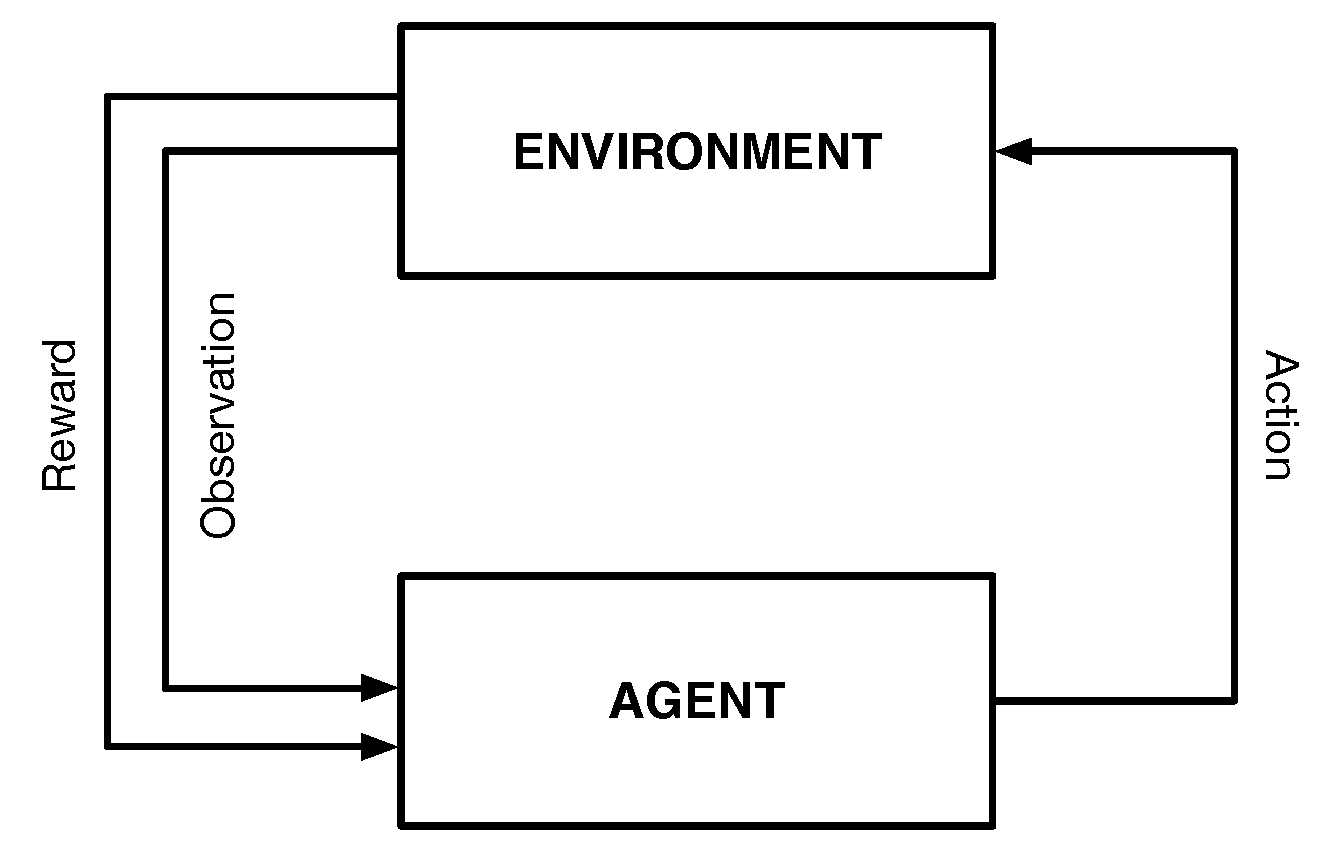
\includegraphics[width=\textwidth]{images/agent-environment.pdf}
\caption{The reinforcement learning process}
\label{fig:agentandenvironment}
\end{figure}
After the action is taken, the state of the environment changes and the agent then receives a new observation of it, and then the process repeats.  The goal of the reinforcement learning agent is to maximize the reward received over a certain time period, finding a balance between immediate and future rewards. 
\end{comment}

Reinforcement learning is an approach to the learning from experience problem in artificial intelligence. A reinforcement learning algorithm's intelligence is built upon having experiences which are then incorporated into the algorithm's own domain knowledge. This knowledge is then used to make intelligent decisions in the future \parencite{barto1998reinforcement}.

\begin{figure}[H]
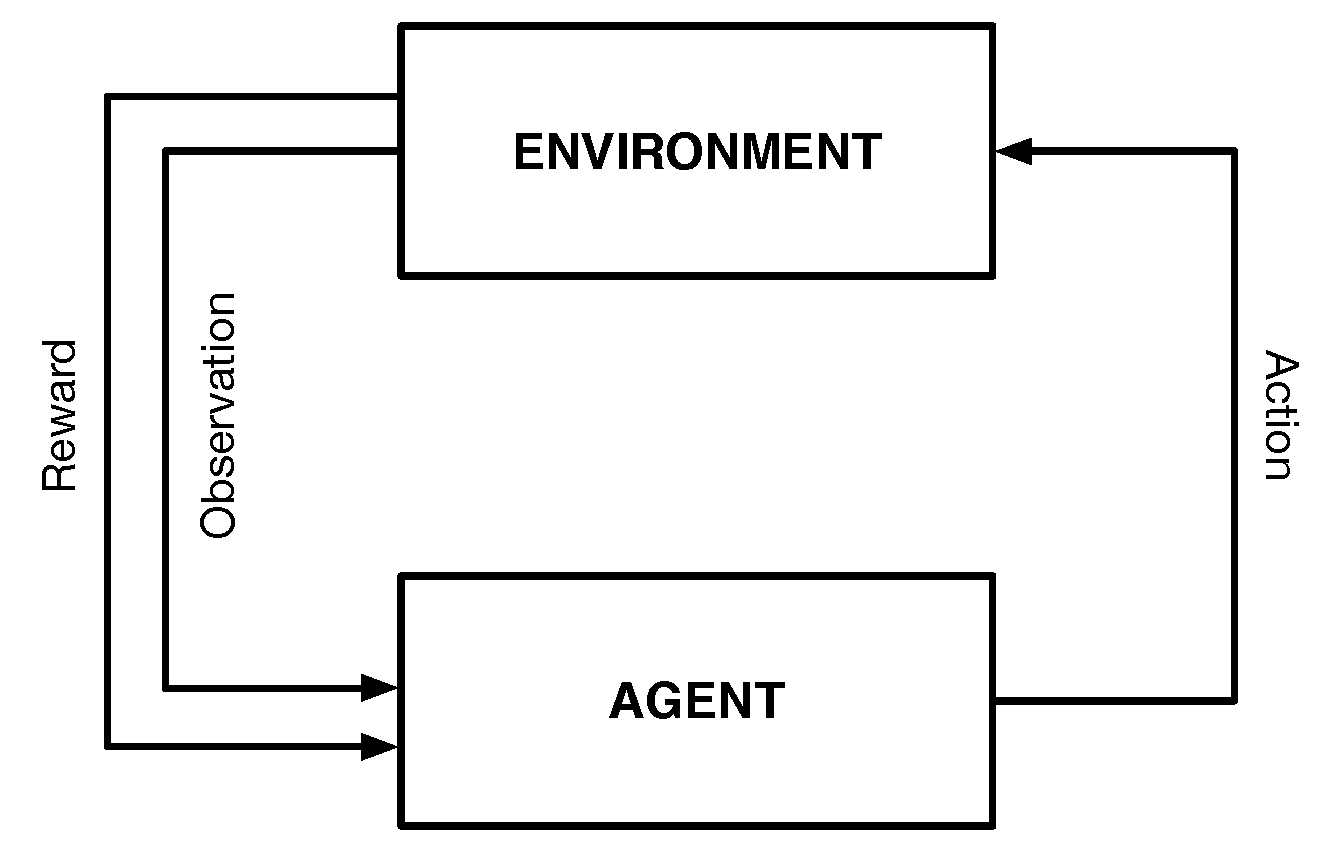
\includegraphics[width=\textwidth]{images/agent-environment.pdf}
\caption{The reinforcement learning process}
\label{fig:agentandenvironment}
\end{figure}

The reinforcement learning problem is modeled as a sequential decision problem, see figure \ref{fig:agentandenvironment} for a graphical representation of the process. A learning algorithm, an agent, performs an action and receives a reward according to some measure of how desirable the results of the action are.  After the action is taken, the state of the environment changes and the agent then receives a new observation of it, and then the process repeats. The goal of the reinforcement learning agent is to maximize the reward received over a certain time period, finding a balance between immediate and future rewards \parencite{barto1998reinforcement}. 


%One thing that sets reinforcement learning apart from other fields within artificial intelligence is that a reinforcement learning problem is solved by an online algorithm. That is, a reinforcement learning algorithm learns about its task and environment while operating in the environment. The actions taken by the agent affect what it knows about the environment, and thus its appraisal of the value of future actions and/or states of the environment.


There are several ways of further dividing reinforcement learning problems into other subcategories. Some examples are the dichotomies 1) episodic/non-episodic problems 2) problems with continuous/discrete state spaces 3) problems with continuous/discrete action spaces 4) problems with one/multiple concurrent agents. (etc.) In the text below, the two first of these dichotomies, which are relevant to this thesis, are discussed. 

\subsection{Episodic and Non-episodic Problems}
One can categorize reinforcement learning problems based on whether or not the time steps are divided into episodes. When the time steps for the agent-environment interaction are divided into subsequences in this manner, the problem is called episodic. This is common in for example games, which end when they are won or lost. If the problem is not episodic, it is called non-episodic, which means, consequently, that the interaction is not divided into subsequences. Instead, the interaction between the actor and environment goes on continually without end \parencite{barto1998reinforcement}. Two examples of non-episodic applications are controlling a robot arm (as well as other robotics problems) and maneuvering a helicopter \parencite{ng2006autonomous}. 

\subsection{Continuous and Discrete Problems}
An alternative way to categorize reinforcement learning problems is based on whether their state spaces are continuous or discrete. An important difference between the two kinds of problems is how an agent can treat similar states in the model. In a continuous problem it is a lot easier to group together states located around the same ``position'' due to the nature of a continuous problem, where the states usually more or less meld together. For example, if the reinforcement learning problem is to control a robot arm whose position is the state of the environment, the different states located around the same general area are not very different. This means that they might be treated in the same way or a similar way by an agent. On the other hand, consider the discrete problem of a game of connect four, wherein the placement of a coin into one of two adjacent slots could dramatically change the evaluation of the state and the outcome of the game \parencite{barto1998reinforcement}.

psection{Markov decision process}

Within reinforcement learning, the concept of Markov secision processes (MDP) is central. An MDP is a way to model an environment where state changes in it are dependent on both random chance and the actions of an agent. An MDP is defined by the quadruple $\left( S, A, P( \cdot , \cdot, \cdot ) , R( \cdot , \cdot ) \right)$ \parencite{altman2002applications}: 

\begin{description}
\item[$S$] \hfill \\ 
    A set of states representing the environment.
\item[$A$] \hfill \\ 
    A set of actions that can be taken.
\item[$P \colon S \times A \times S \to \mathbb R$] \hfill \\ 
    A probability distribution over the transitions in the environment. This function describes the probability of ending up in a certain target state when a certain action is taken from a certain origin state. 
\item[$R \colon S \times A \to \mathbb{R}$] \hfill \\ 
    A function for the reward associated with a state transition. In some formulation of MDPs the reward function only depends on the state.
\end{description}

MDPs are similar to Markov chains, but there are two differences. First, there is a concept of rewards in MDPs, which is absent in Markov chains. Second, in a Markov chain, the only thing that affects the probabilities of transitioning to other states is the current state, whereas in an MPD both the current state and the action taken in that state are needed to know the probability distribution connected with the next state \parencite{altman2002applications}.


\input{Technical_Background/MDP/markov_property.tex}
\input{Technical_Background/MDP/sparse_mdps.tex}
\input{Technical_Background/MDP/factored_representations.tex}


\section{Basic algorithms for solving MDPs}

A policy $\pi$ is a function from a state $s$ to an action $a$ that operates in
the context of a Markov Decision Process, i.e. $\pi \colon S \to A$. A policy
is thus a description of how to act in each state of an MDP. An arbitrary
policy is denoted by $\pi$ and the optimal policy (the policy with the largest
expected reward in the MDP) is denoted by $*$. The rest of this section is
describes some basic algorithms for solving, that is to say finding an optimal
policy, in an MDP.

\subsection{Value functions}

To solve an MDP most algorithms uses an estimation of values of states or
actions. Two value functions are usually defined, the state-value function $V :
S \to \mathbb R$ and the state-action-value function $Q : S \times A \to
\mathbb R$. As the names implies $V$ signifies how good a state is, while $Q$
signifies how good an action in a state is. The state-value function,
$V^\pi(s)$, returns the expected value when starting in state $s$ and following
policy $\pi$ thereafter. Equations \eqref{equation:v_finite} and \eqref{equation:v_infinite} show the equations for the state-value function for a finite time horizon and an infinite, discounted, time horizon respectively. In \eqref{equation:v_infinite}, $\gamma$ is the discount factor, a value between 0 and 1 which describes how fast the value of expected future rewards decay as one looks further into the future. The state-action-value function $Q^\pi(s, a)$ returns
the expected value when starting in state $s$ and taking action $a$ and
thereafter following policy $\pi$. The value functions for the optimal policy
are denoted by $V^*(s)$ and $Q^*(s, a)$. Formulas for the state-action value functions are anologous to those presented for the state value functions. 

\begin{align}
\label{equation:v_finite}
V_t^\pi(s) = \mathbb{E} \{ \sum_{k=0}^{T=k} r_{t+k} | S_t = S, \pi \}
\end{align}

\begin{align}
\label{equation:v_infinite}
V_{0}^\pi(s) = \mathbb{E} \{ \sum_{t=0}^\infty r_{t}\gamma^t | S_0 = S,\pi \}
\end{align}

Both $V^\pi$ and $Q^\pi$ can be estimated from experience. This can be done by
maintaining the average of the rewards that have followed each state when
following the policy $\pi$. When the number of times the state has been
encountered goes to infinity, the average over these histories of rewards
converges to the true values of the value function
\parencite{barto1998reinforcement}.

\input{Technical_Background/ValueFunctions/dynamic_programming.tex}
\input{Technical_Background/ValueFunctions/policy_iteration.tex}
\input{Technical_Background/ValueFunctions/value_iteration.tex}


\subsection{\etre\ in Factored Markov Decision Processes 
\note{N}}
\label{sec:e3_factored_discussion}

\paragraph{General shape of the results} In a comparison of the \etre\ agent's behavior in the different-size environments, the similarity of the shape of the graphs is striking. At first there is a period of lower and lower performance. (For the smallest environments, this period is very short, however.) Next, there is a period of fairly constant high performance, which lasts until the end of the experiment.  

This shape can be explained as a consequence of the different phases of operation of the \etre\ algorithm coupled with the structure of the MDP studied. In the beginning of the experiment, the algorithm will spend almost all of its time in the balanced wandering and exploration phases. The longer the agent has been exploring, and the more states become known, the further the agent has to explore into hard-to-reach parts of the MDP to find unexplored states. Now, in the case of the invasive species environment with the parameters chosen as in the experiments presented, the most easily reachable states are the ones where there is no tamarisk infection. This means that the harder a state is to reach, the more infected it will be, and thus the performance of the \etre\ agent in the exploration phase will fall as the experiment progresses. 

However, once the agent knows enough about the environment to enter the exploitation phase, the \etre\ agent spends close to no time at all exploring unknown states, and it retains high performance. 

\paragraph{Consequences of pooling observation data} An interesting result is that the agent is able to enter the exploitation phase for the 10 reaches/1 habitat per reach test setup slightly earlier than for the 5 reaches/1 habitat per reach setup. This is probably connected to the optimization described in the last paragraph of section \ref{sec:factored_e3}. In the 10 reaches/1 habitat per reach case there are nine reaches with two parents (including the reach itself) and one reach with only itself as parent. In the 5 reaches/1 habitat per reach case there are four reaches with two parents and one reach with only itself as parent. Since observations for state variables with similar parent structure are pooled by our \etre\ implementation, the agent will receive almost double the information per time step for the two-parent reaches in the 10 reaches case as compared to the 5 reaches case.  

\paragraph{Possible issues with the one-policy-per-reach optimization} In section \ref{sec:one_policy_per_state_variable} an optimization is described that works very well for the particular environment and environment settings that the agent was tested for. However, this optimization makes several assumptions that may cause problems if the settings are changed. For instance, one assumption is that the state of a reach is only affected directly by its adjacent parents in the DBN. If the state of a reach was made to depend significantly on other reaches two or more levels up in the river network, the agent would probably not be able to converge on an optimal policy. 

Another assumption that could lead to problems with other environment settings is the assumption that the maximal action cost in the environment is impossible or very hard to break. The invasive species environment has a maximum cost for actions. However, with the standard settings it is mathematically impossible to break this maximum. Our implementation of \etre\ would achieve very poor performance if this was not the case, since a large penalty is given when the maximum action cost is breached. 

\paragraph{DBN structure} Finally, in the invasive species environment, the structure of the DBN underlying the MDP is known at the start of the experiment, so the agent does not need to infer it from its observations. If this was not the case, all the DBN optimizations would be useless unless some kind of algorithm for infering the DBN structure was added to the agent. 

\chapter{Environment and algorithms}
\label{ch:algo}

This chapter gives a description of the environment and the algorithms that
were used in the experiment described in chapter \ref{ch:method}. The environment Invasive Species, is a simulation of a river network with invading species where to goal is to eradicate unwanted species and is further described in section \ref{sec:experiment_env}. 

Two algorithms are covered in this chapter, both of which deal with the
problems that arise with large state spaces; however, they differ in the
methods they apply. In the following chapter the general ideas behind the
algorithms, as well as specific details, are presented. 

The model-based interval estimation algorithm, described in
section~\ref{sec:mbie}, utilizes clever estimations of confidence intervals for
the Q-value functions to improve performance in sparse MDPs.
Section~\ref{sec:fac_e3} is on an algorithm that uses dynamic bayesian networks
and factored representations to improve the \etre\ algorithm to efficiently
deal with factored MDPs. 

\section{Environment specification, Invasive Species}
\label{sec:experiment_env}

When the agents were tested, the Invasive Species environment from the 2014 edition of
the Reinforcement Learning Competition was used. The environment is a
simulation of an invasive species problem, in this case a river network with
invading species where the goal of the agent is to eradicate unwanted species
while replanting native species. 

The environment's model of the river network has parameters, such as the size
of the river network and the rate at which plants spread, which can be
configured in order to create different variations of the environment.  The
size of the river network is defined by two parameters: the number of reaches
and the number of habitats per reach. A habitat is the smallest unit of land
that is considered in the problem. A habitat can either be invaded by the
tamarix, which is an unwanted species, empty or occupied by native species. A
reach is a collection of neighboring habitats. The structure of the river
network is defined in terms of which reach is connected to which
\parencite{invasiveSpecis2014:Online}. In figure \ref{fig:river} a model of a
river network is shown.

\begin{figure}[ht]
\centering
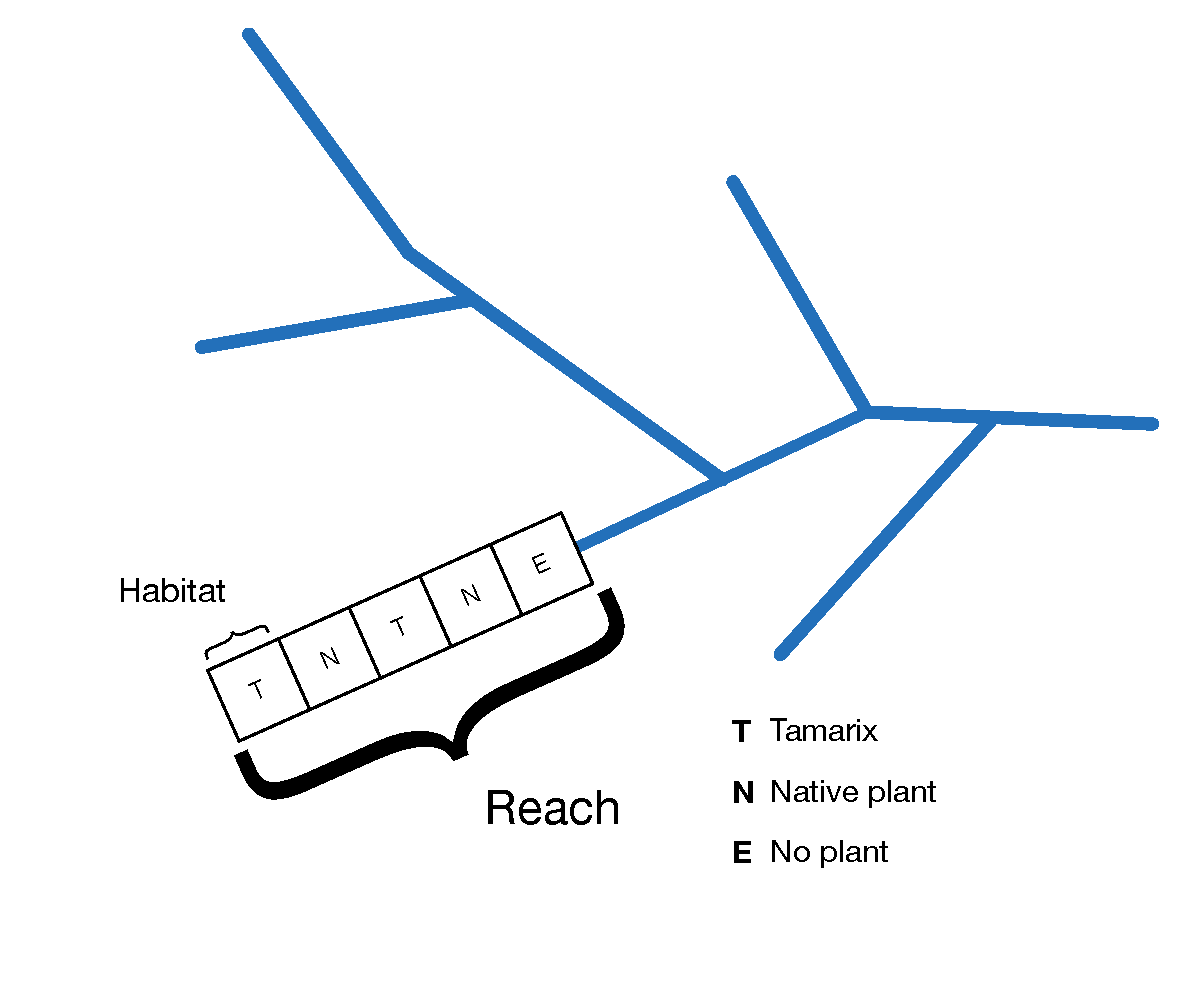
\includegraphics[width=0.9\textwidth]{images/river_network.pdf}
\caption{A river network, as modeled by the Invasive Species reinforcement learning environment.}
\label{fig:river}
\end{figure}

There are four possible actions (eradicate tamarix trees, plant native trees,
eradicate tamarix trees and plant native trees and a wait-and-see action),
and the agent chooses one of these actions for each reach and time step. If the 
agent chooses to eradicate tamarix trees or plant native trees in a reach, 
all habitats of that reach are targeted by this action. What
actions are available to the agent depends on the state of each reach. It is
always possible to choose the wait-and-see action, but there has to be one
or more tamarix-invaded habitats in a reach for the eradicate or eradicate and
plant actions to be available and there has to be at least one empty habitat in
a reach for the plant-native-trees action to be available
\parencite{invasiveSpecis2014:Online}.  

\section{Model-based interval estimation}
\label{sec:mbie}

Model-based interval estimation is a modification of value iteration whose main feature is its  addition of confidence
intervals to the state-action values. These confidence intervals allow the agent to choose between
actions, based on how confident it is about its evaluation of them. In effect,
the less certain the agent is about its evaluation of the states and actions,
the more exploratory the actions will be. When the agent is more confident
however, it will exploit what it has learnt so far about the MDP
\parencite{dietterich2013pac}.

\input{algorithms/MBIE/modification_of_value_it}
\input{algorithms/MBIE/gt.tex}
\input{algorithms/MBIE/modded_bounds}

\section{\etre\ in factored Markov decision processes}
\label{sec:fac_e3}

The second algorithm studied in this thesis is a version of the \etre\ algorithm that focuses on factored problem domains by modeling them as a dynamic Bayesian network. The original \etre\ algorithm is described in section \ref{sec:e3}, which gives a broad overview along with the key strategies used in the algorithm. The following section, \ref{sec:factored_e3}, considers some ways to extend the original algorithm and make use of factored representations and planning in factored domains to improve the running time of the algorithm.

\input{algorithms/Factored_E3/e3.tex}
\input{algorithms/Factored_E3/factored_additions.tex}


\chapter{Method}
\label{sec:method_intro}

This chapter covers the preliminaries and preparations carried out before the
execution of the experiments. It covers  and how the agents described in chapter
\ref{ch:algo} were implemented and the additions and modifications that were made to them. The chapter
concludes with a description of the tools used for the experiment.
\section{Algorithm implementation}
\label{sec:implementation}

We implemented two existing algorithms and we also added some extensions.  The
experiment utilized RL-Glue (section~\ref{sec:rl_glue}) to connect the agents
and environment to each other.  To verify the behavior of our agents we utilized smaller
environments (see sections~\ref{sec:intro_grid_world} and \ref{sec:ns}) where
the correct operation is either easy to derive or obvious from inspection. By
starting with smaller problems and using an iterative approach it was possible
to identify bottlenecks in our implementations and correct possible errors
early.

\input{algorithms/MBIE/modded_bounds}

\input{method/ConstructingExperiments/contributionse3}

\subsection{GridWorld}
\label{sec:intro_grid_world}

The GridWorld environment was implemented to easily be able to verify the
correctness of the MBIE algorithm. It consists of a grid of twelve squares with
one blocked square, one starting square, one winning square, one losing square and
eight empty squares. The agent can take five actions, north, south, west,
east or exit. The exit-action is only possible from the winning or losing
state. When taking an action being in one state and the action is directed to
another empty state there is an 80\% probability to succeed and 10\%
probability to fail and 10\% to go sideways.

\subsection{Network simulator}
\label{sec:ns}

A simple computer network simulation was implemented to verify the behavior of an
early version of \etre\ algorithm. In this environment, the agent tries to keep
a network of computers up and running. All computers start in the running
state, but there is a chance that they randomly stop working. If a computer is
down, it has a chance to cause other computers connected to it to also fail. In
each time step, the agent chooses one computer to restart, which with 100
percent probability will be in working condition in the next time step. The
agent is rewarded for each computer in the running state after each time step. 

\section{Our contributions}
\label{sec:contributions}


\input{algorithms/MBIE/modded_bounds}


\input{method/ConstructingExperiments/contributionse3}

\section{Environment specification}
\label{sec:experiment_env}

For the experiment, the Invasive Species environment from the 2014 edition of
the Reinforcement Learning Competition was used. The environment is a
simulation of an invasive species problem, in this case a river network with
invading species where the goal of the agent is to eradicate unwanted species
while replanting native species. 

The environment's model of the river network has parameters, such as the size
of the river network and the rate at which plants spread, which can be
configured in order to create different variations of the environment.  The
size of the river network is defined by two parameters: the number of reaches
and the number of habitats per reach. A habitat is the smallest unit of land
that is considered in the problem. A habitat can either be invaded by the
tamarix, which is an unwanted species, empty or occupied by native species. A
reach is a collection of neighboring habitats. The structure of the river
network is defined in terms of which reach is connected to which
\parencite{invasiveSpecis2014:Online}. In figure \ref{fig:river} a model of a
river network is shown.

\begin{figure}[ht]
\centering
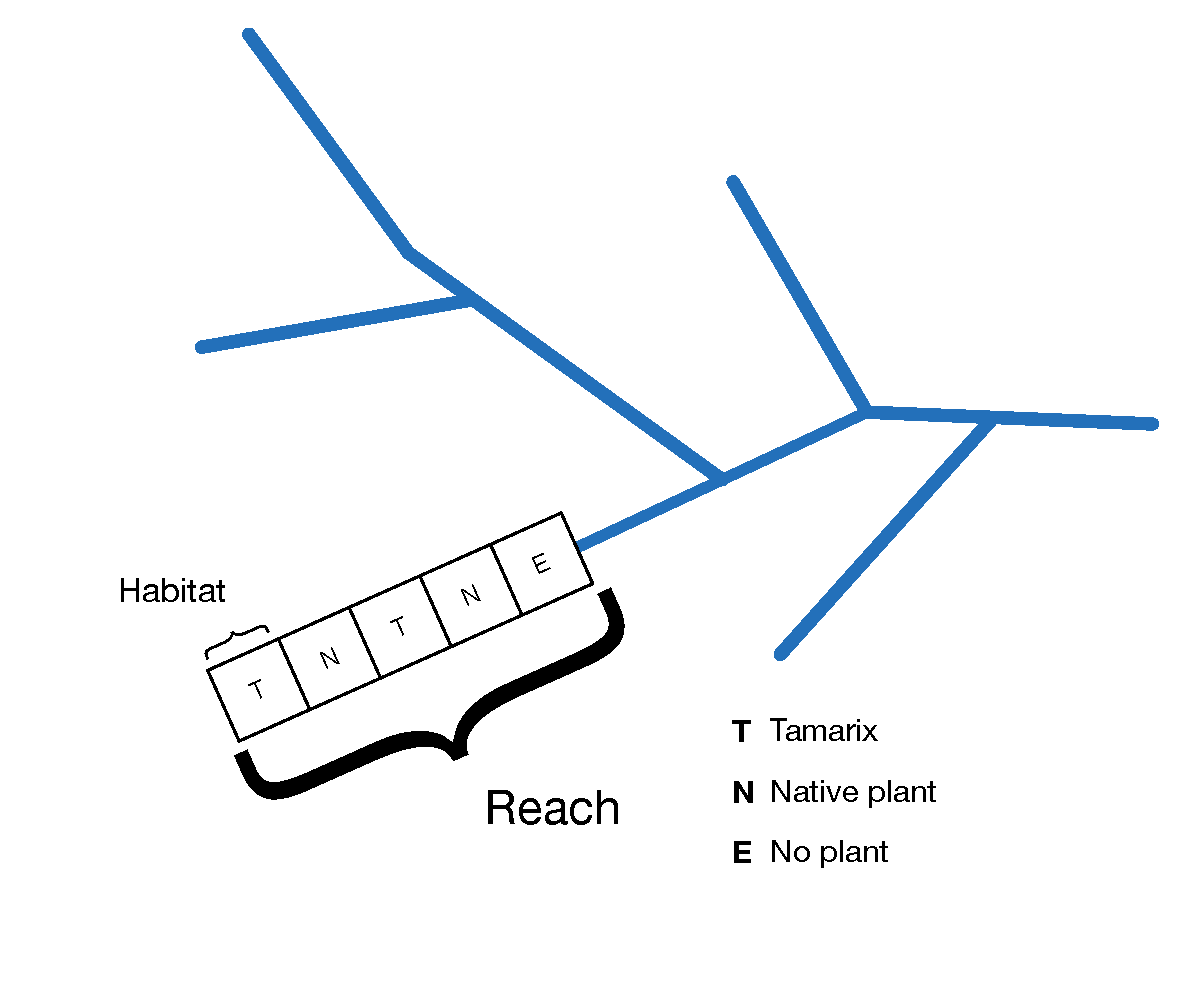
\includegraphics[width=0.9\textwidth]{images/river_network.pdf}
\caption{A river network, as modelled by the Invasive Species reinforcement learning environment.}
\label{fig:river}
\end{figure}

There are four possible actions (eradicate tamarisks, plant native trees,
eradicate tamarisks and plant native trees, and finally a wait-and-see action),
and the agent chooses one of these actions per reach per time step. What
actions are available to the agent depends on the state of each reach. It is
always possible to choose the wait-and-see action, but there has to be one
or more tamarix-invaded habitats in a reach for the eradicate or eradicate and
plant actions to be available and there has to be at least one empty habitat in
a reach for the plant-native-trees action to be avalable
\parencite{invasiveSpecis2014:Online}. 

\section{Test specification}
\label{sec:test_spec}

The testing of the agents required us to choose certain sets of parameters, for
the environment, the two different agents and the experiment itself. 

\paragraph{Environment parameters}

The Invasive Species environment requires a number of parameters. For further
explanation of the environment parameters consult the environment
webpage\footnote{\url{http://2013.rl-competition.org/domains/invasive-species}}.
The specific parameters used are presented in
appendix~\ref{ap:environment_spec}.

\paragraph{Agent Parameters}

The agents evaluated required different types of parameters. Some preliminary
tests were run and then the parameters giving best results were chosen.
Parameters for MBIE are found in table~\ref{tab:mbie_params_both}.

\begin{table}[H]
\centering
\captionof{table}{Parameters for MBIE}
\label{tab:mbie_params_both}

\begin{subfigure}[b]{0.47\textwidth}
    \centering
    \captionof{table}{Proper MBIE}
    \label{tab:mbie_params} 
    \begin{tabular}{lr}
     \toprule
     Parameter & Value \\
     \midrule
     Discount factor, $\gamma$ & 0.9 \\
     Confidence, $\delta$ & 95\% \\
     $\Delta \omega$ & $\frac{1}{2}\sqrt{\frac{2|ln(2^{|S|}-2) - ln  \delta |}{N(s,a)}}$ \\
     
     \bottomrule
    \end{tabular}
\end{subfigure}
\quad
\begin{subfigure}[b]{0.47\textwidth}
    \centering
    \captionof{table}{Realistic MBIE}
    \label{tab:mbie_realistic_params}
    \begin{tabular}{lr}
     \toprule
     Parameter & Value \\
     \midrule
     Discount factor, $\gamma$ & 0.9 \\
     $\Delta \omega$ & $1 - 0.05 N(s,a)$ \\
     \bottomrule
    \end{tabular}
\end{subfigure}
\end{table}

For DBN-\etre\ a higher exploration limit resulted in the agent starting to
exploit earlier but with a slightly lower final return. A higher partial state
known limit resulted in later exploitation but no appreciable difference in
final return. The values in table~\ref{tab:dbne3_params} were a good middle
ground.

\begin{table}[H]
\captionof{table}{DBN-\etre\ parameters}
\label{tab:dbne3_params}
\centering
\begin{tabular}{lr}
 \toprule
 Parameter & Value \\
 \midrule
 Discount factor & 0.9 \\
 Exploration limit & 5\% \\
 Partial state known limit & 5 \\
 \bottomrule
\end{tabular}
\end{table}

\paragraph{Experiment parameters}

The tests performed had to be long enough to sample enough data to extract
relevant results without making the running time too long. A single test
consisted of a specific number of episodes with a specific length. A good
combination was required to efficiently evaluate the agents. If a single
episode consisted of too many samples it would be difficult to see the learning
process as results are reported as total reward over an episode and that
process might be hidden as its impact on the total reward is smaller with a
longer episode. On the other hand, if an episode length is too short it would
end before the agents could do any valuable learning.

In addition to a satisfactory episode length, a reasonable number of episodes
needs to be sampled for it to be possible to draw conclusions from the results.
If the number of episodes is too small, the convergence of the agents cannot be
seen. However, if the number of episodes are too large a lot of sampled data
would be redundant for the study. Some preliminary experiments were run in
order to tune the experiment parameters to suitable values. The episode length
was set to 100 samples and there were 100 episodes per test.

To evaluate the agents in the Invasive Species environment combinations of
reaches and number of habitats per reach that can be seen in
table~\ref{tab:reaches_habitats} were choosen. Combinations were chosen to have
a wide range in the total number of states for the agents to deal with and to
test how the agents deal with taking actions that have to take into account
several state components. 

As seen in table ~\ref{tab:reaches_habitats}, the state count increases rapidly
when habitats are added to the problem. This is obvious from the fact that the state count
depends exponentially on the total number of habitats; see equation \eqref{eq:statecount}, where $h$ is the number of habitats per reach and $r$ is the number of reaches.

\begin{equation}
\label{eq:statecount}
 |S| = 3 ^ {hr}
\end{equation}

\begin{table}[H]
\centering
\caption{Combinations of reaches and habitats used in testing.}
\label{tab:reaches_habitats}
\begin{tabular}{rrr}
 \toprule
 Reaches & Habitats per reach & Total state count \\
 \midrule
 5  & 1 &          243 \\
 3  & 2 &          729 \\
 3  & 3 &      19\,683 \\
 10 & 1 &      59\,049 \\
 4  & 3 &     531\,441 \\
 5  & 3 & 14\,348\,907 \\
 \bottomrule
\end{tabular}
\end{table}

\section{Programming environment}
\label{sec:prog_env}

The Java programming language 1.7 was used to implement the algorithms. In addition, the
Java version of RL-Glue framework version 3.0 was used. For version control Git
was used, due to its simplicity and performance.

\section{RL-Glue}
\label{sec:rl_glue}

To evaluate the agents the RL-Glue framework was used, which acts as an
interface for communication between the agent and the environment. The software
uses the RL-Glue protocol, which specifies how a reinforcement learning problem
should be divided when constructing experiments and how the different programs
should communicate \parencite{tanner2009rl}.

RL-Glue divides the reinforcement learning process into three separate
programs: an agent, an environment and an experiment. RL-Glue provides a server
software that manages the communication between these programs. The agent and
the environment programs are responsible for executing the tasks as specified
by RL-Glue and the experiment program acts as a bridge between the agent and
environment \parencite{tanner2009rl}.

The modular structure of RL-Glue makes it easier to construct repeatable
reinforcement learning experiments. By separating the agent from the
environment it is possible to reuse the environment and switch out the agent.
It also makes it a lot easier to cooperate and continue working on existing
environments implemented by other programmers.


\chapter{Result}

\newcommand{\graphwidth}{0.70\textwidth}
\newcommand{\testsubfigure}[2]{%
\begin{subfigure}[b]{\graphwidth}
    \includegraphics[width=1.1\textwidth]{images/tests/#1r-#2h.pdf}
    \caption{#1 reaches and #2 habitats per reach}
    \label{fig:#1r#2h}
\end{subfigure}
}

In figures~\ref{fig:tests1}, \ref{fig:tests2} and \ref{fig:tests3} we have test results from running our agents on the invasive species environment on different sizes of river network. The raw data can be found in appendix~\ref{ap:result_tables}.

\begin{figure}[h!]
    \centerline{
    \testsubfigure{3}{3}
    ~
    \testsubfigure{3}{2}
    }
    \caption{Test runs with different number of reaches and habitats}
    \label{fig:tests1}
\end{figure}

\begin{figure}[h!]
    \centerline{
    \testsubfigure{5}{1}
    ~
    \testsubfigure{5}{3}
    }
    \caption{Test runs with different number of reaches and habitats}
    \label{fig:tests2}
\end{figure}

\begin{figure}[h!]
    \centerline{
    \testsubfigure{4}{3}
    ~
    \testsubfigure{10}{1}
    }
    \caption{Test runs with different number of reaches and habitats}
    \label{fig:tests3}
\end{figure}

The agent learns for 100 episodes with 100 samples per episode, other parameters are specified in section~\ref{sec:test_spec}. The invasive species environment associates a certain cost with each state and action, thus the reward is always negative. In each test the reward varies over time for the MBIE agent, the realistic MBIE agent and the DBN-\etre\ agent.

With smaller state spaces (see figure~\ref{fig:3r3h}, \ref{fig:3r2h} and \ref{fig:5r1h}) we can see that the realistic MBIE agent outperforms the proper MBIE agent and comes close to the DBN-\etre\ agent. In the tests where the state space is larger (see figure~\ref{fig:5r3h}, \ref{fig:10r1h} and \ref{fig:4r3h}) proper MBIE and realistic MBIE are very close to each other in performance while the DBN-\etre\ agent outperforms both. The realistic MBIE algorithm performs better in with smaller state spaces due to more states becoming known quicker and thus having their true value.

In each of the test runs the DBN-\etre\ algorithm exhibits a period of learning that corresponds to exploration (as described in section~\ref{sec:e3}) where the agent has not explored the environment enough and seeks more information. This is apparent in figure~\ref{fig:3r3h}.
\chapter{Discussion \note{B}}
\label{ch:discussion}
This chapter is a discussion of the results and method used in the project. The algorithms are evaluated with regard to their performance achieved in the tests, which is used as a basis when comparing them against each-other. Determining their strengths and weaknesses and if they were suitable for problems with an environment that has a large discrete state space and in particular for the environment Invasive Species. There is also a discussion on ethical aspects regarding the work in this thesis.


% Det behövs inte en ingående disposition här, det tar ner läsligheten. Det som tas upp i styckena är vettigt, men detta är inte rätt ställe för dem.

% This chapter is a combination of discussion of the results of using the algorithms described in chapter \ref{ch:algo}, together with a examination of the method used in the project. The algorithms is evaluated with regard to their performance achieved in the experiments \ref{sec:constructing_experiments}, which is used for a basis when comparing them against each-other. Focusing on their strengths and weaknesses and circling around the question why did they perform as they did. Were they suitable for this kind of problem, an environment with a large discrete state space and in particular for this thesis a simulation of an Invasive Species environment.

% The second part of this chapter contains a section containing a presentation of similar studies conducted, summarizing their results and opinions. Using their finding as a basis, there will also be a discussion regarding its connection to the results in this thesis. With inspiration from similar studies in combination with the results of this thesis, a discussion about the possible extensions and additional work or unanswered questions in this thesis are presented. 

%In order to round of this chapter, the last section of this chapter revolves around ethical questions and aspects regarding the theme of this topic. The main theme of the last section is ethical aspects in \acrlong{ai} \acrshort{ai}, \acrfull{ai}, along with a discussion about the usefulness of Reinforcement Learning in today's society with focus on using simulations.

\section{Evaluation of the agents \note{I}}
\label{sec:coa}

\input{Discussion/AlgorithmsEvaluation/dbn.tex}
\input{Discussion/AlgorithmsEvaluation/mbie.tex}
\input{Discussion/AlgorithmsEvaluation/discussion_diffrences}




\section{Potential factors impacting the results}
\label{sec:truth_results}

There are several factors that possibly reduce the reliability of the results. For instance, all evaluations used only one environment, the implementation of the algorithms could contain errors and the correct results for all test runs are not always known. 

\input{Discussion/discussion_results/impact_of_one_env.tex}

\input{Discussion/discussion_results/implementation_of_algorithms.tex}

\input{Discussion/discussion_results/testing_methodology.tex}


%\section{Similar Studies \note{N, K}}
The work with reducing the complexity of the reinforcement learning problems with environments containing large state spaces is not a new research topic. However, this thesis is taking a rather uncommon approach to the problem. Instead of trying to derive new algorithms for solving the problem, the focus is instead focused on usefulness of research conducted within the area of reinforcement learning problems. To be even more specific this thesis has zoomed in on two possible attempts on solving the problem with environments containing large state spaces. An approach that is rather uncommon and thus similar studies is as well uncommon. 
%Behöver skrivas om, tydligare
Thereby this section will combining focus on both studies similar to this thesis comparing the usefulness of research already conducted along with a summarized study of studies of work being done to reduce the complexity of environments with large state spaces.

\todo[inline]{Samma miljö kanske, dess pac?}

\paragraph{Similar Studies Regarding Comparing Existing Research}
\todo[inline]{Borde finnas återkoppling i diskussion kring detta}
It has been shown in Strehl and Littman (2004; 2008) that MBIE outperforms \etre\ in the MDPs RiverSwim and SixArms. \parencite{dietterich2013pac}


\paragraph{Large State Spaces using Dynamic Bayesian Networks}
This paragraph is devoted to similar methods using dynamic Bayesian networks as an underlying representation in order to model the structure of the environment. Due to the relevance of using dynamic Bayesian network as a method for tackling similar problems it is thesis on its own in order to summarize them all. It is also possible to study section \ref{sec:better_planing_algos} for further references, however their main focus on the planning algorithm.

An algorithm to DBN-\etre\ is the algorithm by \textcite{ross2012model} which is as well utilizing a factored representation for the underlying structure. However, in the DBN-\etre\ algorithm no planning algorithm was specified and therefore leaving an empty square in the implementation affecting the overall complexity of the algorithm. In the algorithm by \textcite{ross2012model} 

\todo[inline]{Resultatjämförelse}

\paragraph{Similar Studies Regarding Large State Spaces Using Model Based Something grejen}
Grattis MBIE, er punkt.

\section{Ethical and social aspects of artificial intelligence}

\input{Discussion/Ethics/intro.tex}

\input{Discussion/Ethics/invasive_species.tex}

\input{Discussion/Ethics/ai_right_or_wrong.tex}



\section{Further work}

In this section we discuss possible further work and extensions to our thesis.

\input{Discussion/further_work/more_test_envs.tex}
\input{Discussion/further_work/better_planning_dbn.tex}
\input{Discussion/further_work/MBIE.tex}
\input{Discussion/further_work/mbie_should_use_dbn.tex}


\printbibliography

\begin{appendices}

\chapter{Environment specification}
\label{sec:environment_spec}

\begin{table}[H]
\centering
\captionof{table}{Dynamic parameters common to both species}
\label{tab:dynamic_params_common} 
\begin{tabular}{l r}
 \toprule
 Parameter & Value \\
 \midrule
 Eradication rate & 0.85 \\
 Restoration rate & 0.65 \\
 Downstream spread rate & 0.5 \\
 Upstream spread rate & 0.1 \\
 \bottomrule
\end{tabular}
\end{table}

\begin{table}[H]
\centering
\captionof{table}{Dynamic parameters different between the species} \label{tab:dynamic_params_not_common}
\begin{tabular}{lrr}
\toprule
 Parameter & Native & Tamarisk \\
 \midrule
 Death rate & 0.2 & 0.2 \\
 Production rate & 200 & 200 \\
 Exogenous arrival\footnote{Arrival of seeds from outside the environment} & Yes & Yes \\
 Exogenous arrival probability & 0.1 & 0.1 \\
 Exogenous arrival number & 150 & 150 \\
 \bottomrule
\end{tabular}
\end{table}

\begin{table}[H]
\centering
\captionof{table}{Cost function parameters} \label{tab:cost_params} 
\begin{tabular}{lr}
 \toprule
 Parameter & Value \\
 \midrule
 Cost per invaded reach & 10 \\
 Cost per tree & 0.1 \\
 Cost per empty slot & 0.01 \\
 Eradication cost & 0.5 \\
 Restoration cost & 0.9 \\
 \bottomrule
\end{tabular}
\end{table}

\begin{table}[H]
\centering
 \captionof{table}{Variable costs depending on number of habitats affected by action}
 \begin{tabular}{lr}
 \toprule
 Parameter & Value \\
 \midrule
 Eradication cost & 0.4 \\
 Restoration cost for empty slot & 0.4 \\
 Restoration cost for invaded slot & 0.8 \\
 \bottomrule
\end{tabular}
\label{tab:cost_params_var}
\end{table}
\end{appendices}


\end{document}


\printbibliography

\begin{appendices}

\chapter{Environment specification}
\label{sec:environment_spec}

\begin{table}[H]
\centering
\captionof{table}{Dynamic parameters common to both species}
\label{tab:dynamic_params_common} 
\begin{tabular}{l r}
 \toprule
 Parameter & Value \\
 \midrule
 Eradication rate & 0.85 \\
 Restoration rate & 0.65 \\
 Downstream spread rate & 0.5 \\
 Upstream spread rate & 0.1 \\
 \bottomrule
\end{tabular}
\end{table}

\begin{table}[H]
\centering
\captionof{table}{Dynamic parameters different between the species} \label{tab:dynamic_params_not_common}
\begin{tabular}{lrr}
\toprule
 Parameter & Native & Tamarisk \\
 \midrule
 Death rate & 0.2 & 0.2 \\
 Production rate & 200 & 200 \\
 Exogenous arrival\footnote{Arrival of seeds from outside the environment} & Yes & Yes \\
 Exogenous arrival probability & 0.1 & 0.1 \\
 Exogenous arrival number & 150 & 150 \\
 \bottomrule
\end{tabular}
\end{table}

\begin{table}[H]
\centering
\captionof{table}{Cost function parameters} \label{tab:cost_params} 
\begin{tabular}{lr}
 \toprule
 Parameter & Value \\
 \midrule
 Cost per invaded reach & 10 \\
 Cost per tree & 0.1 \\
 Cost per empty slot & 0.01 \\
 Eradication cost & 0.5 \\
 Restoration cost & 0.9 \\
 \bottomrule
\end{tabular}
\end{table}

\begin{table}[H]
\centering
 \captionof{table}{Variable costs depending on number of habitats affected by action}
 \begin{tabular}{lr}
 \toprule
 Parameter & Value \\
 \midrule
 Eradication cost & 0.4 \\
 Restoration cost for empty slot & 0.4 \\
 Restoration cost for invaded slot & 0.8 \\
 \bottomrule
\end{tabular}
\label{tab:cost_params_var}
\end{table}
\end{appendices}


\end{document}
